\documentclass[dutch]{style/tudelft-report}

\usepackage{acronym}
\usepackage{wrapfig}
\acrodef{sig}[SIG]{Software Improvement Group}
\acrodef{rx}[Rx]{Reactive Extensions}
\acrodef{tfs}[TFS]{Team Foundation Server}
\acrodef{mvp}[MVP]{Minimum Viable Product}
\acrodef{paas}[PaaS]{Platform as a Service}
\acrodef{KNSB}[KNSB]{Koninklijke Nederlandsche Schaatsenrijders Bond}
\acrodef{pcl}[PCL]{Portable Class Library}
%\acrodef{label}[acronym]{written out form}
\usepackage{longtable}
\usepackage{array}
\newcolumntype{R}{>{\raggedleft\arraybackslash}p{5cm}}
\usepackage{subfigure}
\usepackage{float}
\usepackage{xspace}

\usepackage{fancyvrb}

\makeatletter
\def\PY@reset{\let\PY@it=\relax \let\PY@bf=\relax%
    \let\PY@ul=\relax \let\PY@tc=\relax%
    \let\PY@bc=\relax \let\PY@ff=\relax}
\def\PY@tok#1{\csname PY@tok@#1\endcsname}
\def\PY@toks#1+{\ifx\relax#1\empty\else%
    \PY@tok{#1}\expandafter\PY@toks\fi}
\def\PY@do#1{\PY@bc{\PY@tc{\PY@ul{%
    \PY@it{\PY@bf{\PY@ff{#1}}}}}}}
\def\PY#1#2{\PY@reset\PY@toks#1+\relax+\PY@do{#2}}

\expandafter\def\csname PY@tok@gd\endcsname{\def\PY@tc##1{\textcolor[rgb]{0.63,0.00,0.00}{##1}}}
\expandafter\def\csname PY@tok@gu\endcsname{\let\PY@bf=\textbf\def\PY@tc##1{\textcolor[rgb]{0.50,0.00,0.50}{##1}}}
\expandafter\def\csname PY@tok@gt\endcsname{\def\PY@tc##1{\textcolor[rgb]{0.00,0.27,0.87}{##1}}}
\expandafter\def\csname PY@tok@gs\endcsname{\let\PY@bf=\textbf}
\expandafter\def\csname PY@tok@gr\endcsname{\def\PY@tc##1{\textcolor[rgb]{1.00,0.00,0.00}{##1}}}
\expandafter\def\csname PY@tok@cm\endcsname{\let\PY@it=\textit\def\PY@tc##1{\textcolor[rgb]{0.38,0.63,0.69}{##1}}}
\expandafter\def\csname PY@tok@vg\endcsname{\def\PY@tc##1{\textcolor[rgb]{0.73,0.38,0.84}{##1}}}
\expandafter\def\csname PY@tok@m\endcsname{\def\PY@tc##1{\textcolor[rgb]{0.25,0.63,0.44}{##1}}}
\expandafter\def\csname PY@tok@mh\endcsname{\def\PY@tc##1{\textcolor[rgb]{0.25,0.63,0.44}{##1}}}
\expandafter\def\csname PY@tok@cs\endcsname{\def\PY@tc##1{\textcolor[rgb]{0.38,0.63,0.69}{##1}}\def\PY@bc##1{\setlength{\fboxsep}{0pt}\colorbox[rgb]{1.00,0.94,0.94}{\strut ##1}}}
\expandafter\def\csname PY@tok@ge\endcsname{\let\PY@it=\textit}
\expandafter\def\csname PY@tok@vc\endcsname{\def\PY@tc##1{\textcolor[rgb]{0.73,0.38,0.84}{##1}}}
\expandafter\def\csname PY@tok@il\endcsname{\def\PY@tc##1{\textcolor[rgb]{0.25,0.63,0.44}{##1}}}
\expandafter\def\csname PY@tok@go\endcsname{\def\PY@tc##1{\textcolor[rgb]{0.53,0.53,0.53}{##1}}}
\expandafter\def\csname PY@tok@cp\endcsname{\def\PY@tc##1{\textcolor[rgb]{0.00,0.44,0.13}{##1}}}
\expandafter\def\csname PY@tok@gi\endcsname{\def\PY@tc##1{\textcolor[rgb]{0.00,0.63,0.00}{##1}}}
\expandafter\def\csname PY@tok@gh\endcsname{\let\PY@bf=\textbf\def\PY@tc##1{\textcolor[rgb]{0.00,0.00,0.50}{##1}}}
\expandafter\def\csname PY@tok@ni\endcsname{\let\PY@bf=\textbf\def\PY@tc##1{\textcolor[rgb]{0.84,0.33,0.22}{##1}}}
\expandafter\def\csname PY@tok@nl\endcsname{\let\PY@bf=\textbf\def\PY@tc##1{\textcolor[rgb]{0.00,0.13,0.44}{##1}}}
\expandafter\def\csname PY@tok@nn\endcsname{\let\PY@bf=\textbf\def\PY@tc##1{\textcolor[rgb]{0.05,0.52,0.71}{##1}}}
\expandafter\def\csname PY@tok@no\endcsname{\def\PY@tc##1{\textcolor[rgb]{0.38,0.68,0.84}{##1}}}
\expandafter\def\csname PY@tok@na\endcsname{\def\PY@tc##1{\textcolor[rgb]{0.25,0.44,0.63}{##1}}}
\expandafter\def\csname PY@tok@nb\endcsname{\def\PY@tc##1{\textcolor[rgb]{0.00,0.44,0.13}{##1}}}
\expandafter\def\csname PY@tok@nc\endcsname{\let\PY@bf=\textbf\def\PY@tc##1{\textcolor[rgb]{0.05,0.52,0.71}{##1}}}
\expandafter\def\csname PY@tok@nd\endcsname{\let\PY@bf=\textbf\def\PY@tc##1{\textcolor[rgb]{0.33,0.33,0.33}{##1}}}
\expandafter\def\csname PY@tok@ne\endcsname{\def\PY@tc##1{\textcolor[rgb]{0.00,0.44,0.13}{##1}}}
\expandafter\def\csname PY@tok@nf\endcsname{\def\PY@tc##1{\textcolor[rgb]{0.02,0.16,0.49}{##1}}}
\expandafter\def\csname PY@tok@si\endcsname{\let\PY@it=\textit\def\PY@tc##1{\textcolor[rgb]{0.44,0.63,0.82}{##1}}}
\expandafter\def\csname PY@tok@s2\endcsname{\def\PY@tc##1{\textcolor[rgb]{0.25,0.44,0.63}{##1}}}
\expandafter\def\csname PY@tok@vi\endcsname{\def\PY@tc##1{\textcolor[rgb]{0.73,0.38,0.84}{##1}}}
\expandafter\def\csname PY@tok@nt\endcsname{\let\PY@bf=\textbf\def\PY@tc##1{\textcolor[rgb]{0.02,0.16,0.45}{##1}}}
\expandafter\def\csname PY@tok@nv\endcsname{\def\PY@tc##1{\textcolor[rgb]{0.73,0.38,0.84}{##1}}}
\expandafter\def\csname PY@tok@s1\endcsname{\def\PY@tc##1{\textcolor[rgb]{0.25,0.44,0.63}{##1}}}
\expandafter\def\csname PY@tok@gp\endcsname{\let\PY@bf=\textbf\def\PY@tc##1{\textcolor[rgb]{0.78,0.36,0.04}{##1}}}
\expandafter\def\csname PY@tok@sh\endcsname{\def\PY@tc##1{\textcolor[rgb]{0.25,0.44,0.63}{##1}}}
\expandafter\def\csname PY@tok@ow\endcsname{\let\PY@bf=\textbf\def\PY@tc##1{\textcolor[rgb]{0.00,0.44,0.13}{##1}}}
\expandafter\def\csname PY@tok@sx\endcsname{\def\PY@tc##1{\textcolor[rgb]{0.78,0.36,0.04}{##1}}}
\expandafter\def\csname PY@tok@bp\endcsname{\def\PY@tc##1{\textcolor[rgb]{0.00,0.44,0.13}{##1}}}
\expandafter\def\csname PY@tok@c1\endcsname{\let\PY@it=\textit\def\PY@tc##1{\textcolor[rgb]{0.38,0.63,0.69}{##1}}}
\expandafter\def\csname PY@tok@kc\endcsname{\let\PY@bf=\textbf\def\PY@tc##1{\textcolor[rgb]{0.00,0.44,0.13}{##1}}}
\expandafter\def\csname PY@tok@c\endcsname{\let\PY@it=\textit\def\PY@tc##1{\textcolor[rgb]{0.38,0.63,0.69}{##1}}}
\expandafter\def\csname PY@tok@mf\endcsname{\def\PY@tc##1{\textcolor[rgb]{0.25,0.63,0.44}{##1}}}
\expandafter\def\csname PY@tok@err\endcsname{\def\PY@bc##1{\setlength{\fboxsep}{0pt}\fcolorbox[rgb]{1.00,0.00,0.00}{1,1,1}{\strut ##1}}}
\expandafter\def\csname PY@tok@kd\endcsname{\let\PY@bf=\textbf\def\PY@tc##1{\textcolor[rgb]{0.00,0.44,0.13}{##1}}}
\expandafter\def\csname PY@tok@ss\endcsname{\def\PY@tc##1{\textcolor[rgb]{0.32,0.47,0.09}{##1}}}
\expandafter\def\csname PY@tok@sr\endcsname{\def\PY@tc##1{\textcolor[rgb]{0.14,0.33,0.53}{##1}}}
\expandafter\def\csname PY@tok@mo\endcsname{\def\PY@tc##1{\textcolor[rgb]{0.25,0.63,0.44}{##1}}}
\expandafter\def\csname PY@tok@mi\endcsname{\def\PY@tc##1{\textcolor[rgb]{0.25,0.63,0.44}{##1}}}
\expandafter\def\csname PY@tok@kn\endcsname{\let\PY@bf=\textbf\def\PY@tc##1{\textcolor[rgb]{0.00,0.44,0.13}{##1}}}
\expandafter\def\csname PY@tok@o\endcsname{\def\PY@tc##1{\textcolor[rgb]{0.40,0.40,0.40}{##1}}}
\expandafter\def\csname PY@tok@kr\endcsname{\let\PY@bf=\textbf\def\PY@tc##1{\textcolor[rgb]{0.00,0.44,0.13}{##1}}}
\expandafter\def\csname PY@tok@s\endcsname{\def\PY@tc##1{\textcolor[rgb]{0.25,0.44,0.63}{##1}}}
\expandafter\def\csname PY@tok@kp\endcsname{\def\PY@tc##1{\textcolor[rgb]{0.00,0.44,0.13}{##1}}}
\expandafter\def\csname PY@tok@w\endcsname{\def\PY@tc##1{\textcolor[rgb]{0.73,0.73,0.73}{##1}}}
\expandafter\def\csname PY@tok@kt\endcsname{\def\PY@tc##1{\textcolor[rgb]{0.56,0.13,0.00}{##1}}}
\expandafter\def\csname PY@tok@sc\endcsname{\def\PY@tc##1{\textcolor[rgb]{0.25,0.44,0.63}{##1}}}
\expandafter\def\csname PY@tok@sb\endcsname{\def\PY@tc##1{\textcolor[rgb]{0.25,0.44,0.63}{##1}}}
\expandafter\def\csname PY@tok@k\endcsname{\let\PY@bf=\textbf\def\PY@tc##1{\textcolor[rgb]{0.00,0.44,0.13}{##1}}}
\expandafter\def\csname PY@tok@se\endcsname{\let\PY@bf=\textbf\def\PY@tc##1{\textcolor[rgb]{0.25,0.44,0.63}{##1}}}
\expandafter\def\csname PY@tok@sd\endcsname{\let\PY@it=\textit\def\PY@tc##1{\textcolor[rgb]{0.25,0.44,0.63}{##1}}}

\def\PYZbs{\char`\\}
\def\PYZus{\char`\_}
\def\PYZob{\char`\{}
\def\PYZcb{\char`\}}
\def\PYZca{\char`\^}
\def\PYZam{\char`\&}
\def\PYZlt{\char`\<}
\def\PYZgt{\char`\>}
\def\PYZsh{\char`\#}
\def\PYZpc{\char`\%}
\def\PYZdl{\char`\$}
\def\PYZhy{\char`\-}
\def\PYZsq{\char`\'}
\def\PYZdq{\char`\"}
\def\PYZti{\char`\~}
% for compatibility with earlier versions
\def\PYZat{@}
\def\PYZlb{[}
\def\PYZrb{]}
\makeatother

\begin{document}

\def \mylaps {MyLaps\xspace}

%% Use Roman numerals for the page numbers of the title pages and table of
%% contents.
\frontmatter

\title[Bachelorproject]{Vantage Practice}
\author{H.J.\ Banken \\ P.A.\ van Hesteren \\ H.T.D.\ Visser}
\affiliation{Technische Universiteit Delft}
\coverimage{style/cover.jpg}
\makecover

\begin{titlepage}

\begin{center}

%% Insert the TU Delft logo at the bottom of the page.
\begin{tikzpicture}[remember picture,overlay]
    \node at (current page.south)[anchor=south,inner sep=0pt]{
        
\includegraphics{style/cover/logo}
    };
\end{tikzpicture}

\begin{tikzpicture}[remember picture,overlay]
    \node at (current page.south)[anchor=south,inner sep=80pt]{
        
\includegraphics[scale=0.7]{style/cover/emando}
    };
\end{tikzpicture}

%% Extra whitespace at the top.
\vspace*{2\bigskipamount}

%% Print the title in cyan.
{\makeatletter
\titlestyle\color{tudelft-cyan}\Huge\@title
\makeatother}

\bigskip
\bigskip

{\makeatletter
\titlestyle\color{tudelft-cyan}\LARGE Trainingsapp voor Baansporten
\makeatother}

%% Print the optional subtitle in black.
{\makeatletter
\ifx\@subtitle\undefined\else
    \bigskip
    \titlefont\titleshape\Large\@subtitle
\fi
\makeatother}

\bigskip
\bigskip

%by
door

\bigskip
\bigskip

%% Print the name of the author.
{\makeatletter
\titlefont\Large\bfseries Herman Banken
\makeatother}

\bigskip

{\makeatletter
\titlefont\Large\bfseries Patrick van Hesteren
\makeatother}

\bigskip

{\makeatletter
\titlefont\Large\bfseries Hylke Visser
\makeatother}

\vfill

\begin{tabular}{lll}
%% Add additional information here, per faculty requirements, e.g
%    Student number: & 1234567 \\
%    Project duration: & \multicolumn{2}{l}{March 1, 2012 -- January 1, 2013} \\
    TU Coach: & Dr.ir. C.\ Bezemer \\
    Projectbegeleider: & J.\ Stokking
\end{tabular}

%% Only include the following lines if confidentiality is applicable.
\bigskip
\bigskip
%\emph{This thesis is confidential and cannot be made public until December 31, 2013.}
%\emph{Op dit verslag is geheimhouding van toepassing tot en met 31 december 2013.}

\bigskip
\bigskip

\bigskip
\bigskip
%An electronic version of this thesis is available at \url{http://repository.tudelft.nl/}.
%Een elektronische versie van dit verslag is beschikbaar op \url{http://repository.tudelft.nl/}.

\end{center}

\end{titlepage}

\chapter*{Voorwoord}
\setheader{Voorwoord}

Dit document is het eindverslag van het bachelorproject ``Trainingsapp voor Baansporten'', van de opleiding Technische Informatica op de TU Delft, uitgevoerd door Herman Banken, Patrick van Hesteren en Hylke Visser.

\medskip

\noindent We willen graag de volgende personen bedanken voor hun steun en begeleiding gedurende het project:

\medskip

\noindent

\begin{description}

\item[Coach (TU Delft): dr. ir. Cor-Paul Bezemer] ~ \\
Als TU Coach heeft Cor-Paul een grote rol gespeeld binnen het traject van het project. Naast het toezicht houden op het proces, heeft hij ons wekelijks voorzien van feedback op de voortgang van het project. Tevens heeft bij het schrijven van dit document en het voorbereiden van de gebruikerstest voorzien van tips en feedback.

\medskip

\item[Projectbegeleider (Eigenaar Emando): Johan Stokking] ~ \\
Als projectbegeleider heeft Johan een belangrijke rol gespeeld binnen het ontwikkeltraject van het project. Naast het toezichthouden op de kwaliteit en voortgang van het project, heeft hij een actieve rol gespeeld binnen zowel het implementatie- als het ontwerp-proces van de applicatie.

\end{description}

\medskip

Daarnaast willen we Martha Larson, dr. ir. Johan Pouwelse en Marleen Banken bedanken voor de tijd en moeite die zij in ons project hebben gestoken. 

\bigskip

\begin{flushright}
{\makeatletter\itshape
    \@author \\
    Delft, 19 Juni 2014
\makeatother}
\end{flushright}

\tableofcontents

\chapter*{Samenvatting}
\setheader{Samenvatting}

In baansporten is de laatste jaren een ontwikkeling gaande om tijdregistratie te digitaliseren door het gebruik van transponders en detectie-lussen (in de baan). Door deze ontwikkeling zijn nieuwe mogelijkheden ontstaan om ook naast het wedstrijdmoment de sportprestaties in te zien.

Het huidige gebruik van transponders - buiten wedstrijden - is voornamelijk achteraf, terwijl juist tijdens de training zowel sporter als coach het meeste bezig zijn met de prestaties. Het is daarom wenselijk om de resultaten in real-time door te geven aan coaches en sporters zelf. De bestaande oplossingen bieden slechts beperkt inzicht in trainingen, hetgeen de aanleiding voor dit Bachelor Eind Project is geweest.\\

\noindent 
Gedurende dit project is met hulp van de agile ontwikkelmethode SCRUM in combinatie met Team Foundation Server gewerkt aan een applicatie die op een overzichtelijke manier inzicht geeft in trainingen van eigen, maar ook andere sporters. Daarnaast bevat de applicatie een sociale component, waarmee sporters gemotiveerd worden om te blijven/gaan sporten.

Gebruikers kunnen een transponder toekennen aan hun account en groepen aan te maken en/of hier deel in te nemen. Deze groepen bieden hen de mogelijkheid om naast hun eigen resultaten ook andermans resultaten in te zien. Bijvoorbeeld een coach en zijn pupillen. Tevens kunnen zij zich abonneren op andere sporters, handig voor het thuisfront.

Daarnaast bevat dit sociale component ook de mogelijkheid om leaderboards, een soort ranglijst, per verschillende context in te zien. Zo heeft iedere gebruiker zijn eigen records, maar heeft hij ook een positie op de ranglijst van de banen waarop hij gesport heeft en in de groepen waarvan hij deel uitmaakt.\\

\noindent
Om sporters reeds tijdens hun training inzicht te geven in hun prestaties dient alle verkregen data realtime verwerkt en verstuurd te worden naar de mobiele telefoons. Om dit mogelijk te maken draait er in de Microsoft Azure Cloud een server die transponder-doorkomsten verwerkt. De doorkomsten komen binnen vanuit MyLaps, de transponder- en detectielussenleverancier. Vervolgens groeperen we doorkomsten op trainingssessies en ronden, en onderscheiden we de rustperiodes. Het verwerkingsproces steekt vernuftig in elkaar: de beschikbare data wordt steeds een beetje meer verrijkt en steeds naar de applicaties verstuurd.

De applicatie is ontwikkeld met behulp van cross-platform ontwikkel-technieken, waardoor deze relatief eenvoudig uit te brengen is op andere mobiele platformen. De back-end van de applicatie is sport-agnostisch, waardoor deze breed inzetbaar is voor allerlei verschillende soorten baansporten. \\

\noindent 
Uit de enquêtes, die gedurende het project afgenomen zijn onder de doelgroep van de applicatie, is gebleken dat er veel vraag naar een dergelijke applicatie is en de applicatie veel potentie heeft. Ook is er tijdens meetings tussen Emando, de opdrachtgever, en de \ac{KNSB} naar voren gekomen dat de \ac{KNSB} veel interesse heeft in de applicatie en de doorontwikkeling ervan.

Momenteel is de iPhone applicatie klaar om de markt op te gaan, maar uit de enquêtes en vanuit de \ac{KNSB} is naar voren gekomen dat er nog veel functionaliteit is die toegevoegd zou kunnen worden aan de applicatie. Onze aanbeveling is dan ook om de applicatie verder te ontwikkelen en de doelgroep te vergroten door de applicatie ook uit te brengen voor andere platformen.



%% Use Arabic numerals for the page numbers of the chapters.
\mainmatter

\chapter{Inleiding} \label{ch:inleiding} \newcommand{\aanleiding}{}

\begin{wrapfigure}{r}{4cm}
  \begin{center}
    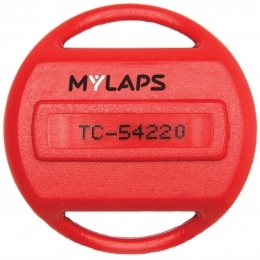
\includegraphics[width=4cm]{style/images/transponder}
  \end{center}
  \caption{MyLaps ProFlex transponder, op schaal}
  \label{fig:transponder}
  \vspace{15mm}
\end{wrapfigure}

In baansporten is de laatste jaren een ontwikkeling gaande om tijdregistratie te digitaliseren door het gebruik van transponders (bijvoorbeeld de MyLaps ProFlex transponder in Figuur~\ref{fig:transponder}) en detectie-lussen (Figuur~\ref{fig:detection-loop}) in de baan. Door deze ontwikkeling zijn nieuwe mogelijkheden ontstaan om ook naast het wedstrijdmoment de sportprestaties in te zien. Het constateren van de hierna genoemde nieuwe mogelijkheden was de aanleiding van dit project.

\begin{wrapfigure}{r}{4cm}
  \begin{center}
    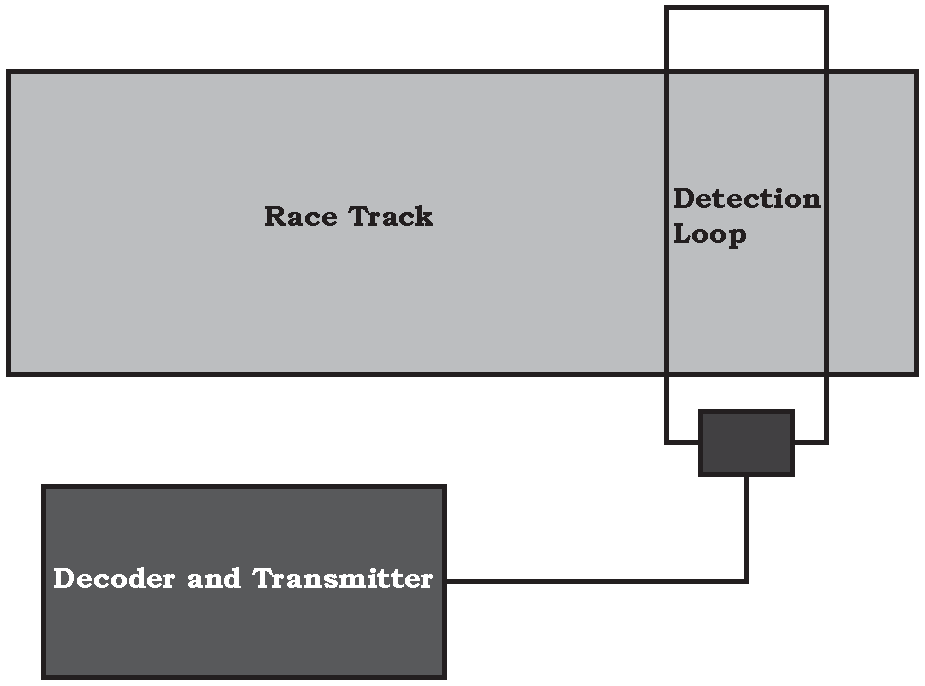
\includegraphics[width=4cm]{style/images/DetectionLoop}
  \end{center}
  \caption{Een schema van een detectielus en en decoder}
  \label{fig:detection-loop}
  \vspace{5mm}
\end{wrapfigure}

Een grote speler op de tijdregistratie-markt is MyLaps\footnote{\url{http://www.mylaps.com}}. Dit bedrijf installeert en beheert detectie-lussen en is actief bij diverse sporten zoals schaatsen, wielrennen, zwemmen, atletiek en diverse motorsporten. Bij sporten met permanente banen liggen de detectie-lussen het gehele jaar in de baan. Er bestaat de mogelijkheid om op de website van MyLaps doorkomst-tijden in te zien. De informatie die uit deze tijden is af te leiden, wordt door sporters als erg waardevol gezien om zich willen blijven verbeteren, waardoor er steeds meer getraind wordt met deze transponders.

\begin{figure}
  \begin{center}
    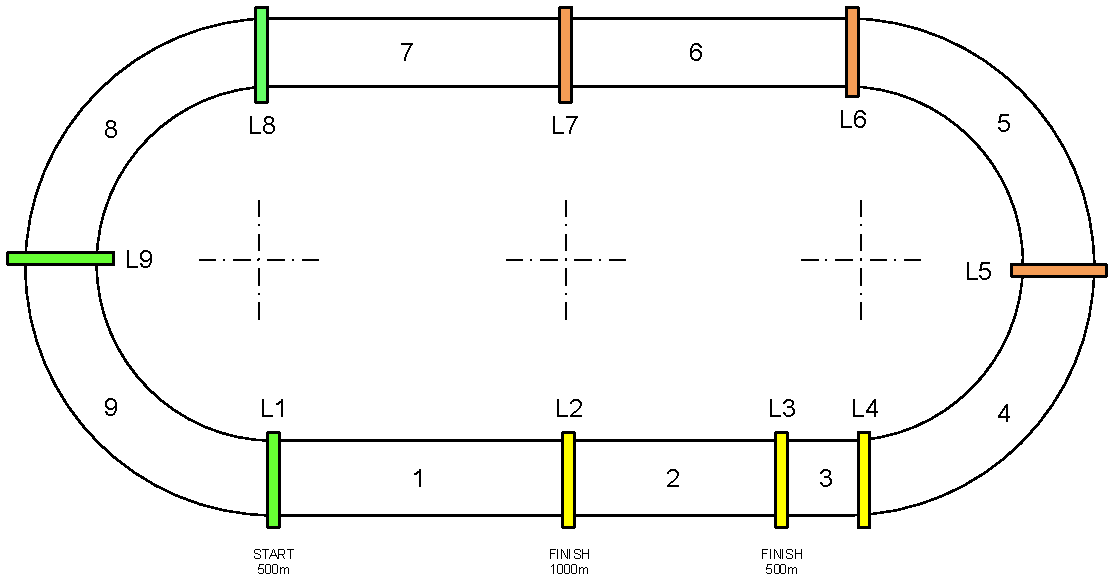
\includegraphics[width=0.8\textwidth]{style/images/BaanoverzichtHaarlem}
  \end{center}
  \caption{L1 tot en met L9 zijn de negen MyLaps transponderlussen in Haarlem}
  \label{fig:track-transponders}
\end{figure}

Voor aanvang van het seizoen worden door MyLaps detectielussen geïnstalleerd. De lussen bevinden zich in het ijs of onder het houten oppervlak van een baanwielrenbaan. Elke lus heeft een elektromagnetisch veld. Wanneer een sporter met transponder over dat veld heen rijdt, wordt de transponder geactiveerd en stuurt deze een unieke puls, die de lus opvangt. De MyLaps X2 server die aan de lussen zit aangesloten stuurt vervolgens het signaal door naar de MyLaps Cloud.

Het huidige gebruik van transponders - buiten wedstrijden - is voornamelijk achteraf, terwijl juist tijdens de training zowel sporter als coach het meeste bezig zijn met de prestaties. Het is daarom wenselijk om de resultaten in real-time door te geven aan coaches en sporters zelf.

Op veel banen zijn meerdere detectie-lussen geïnstalleerd, terwijl er op de website van MyLaps slechts één wordt ontsloten. In Thialf, de schaatsbaan in Heerenveen, Friesland, liggen bijvoorbeeld twaalf detectie-lussen, in Haarlem (Figuur~\ref{fig:track-transponders}) negen en op de andere schaatsbanen liggen er tenminste twee. Door de data van meerdere lussen te combineren is een betere indicatie te maken van de snelheid van sporters.

\begin{wrapfigure}{r}{0.4\textwidth}
 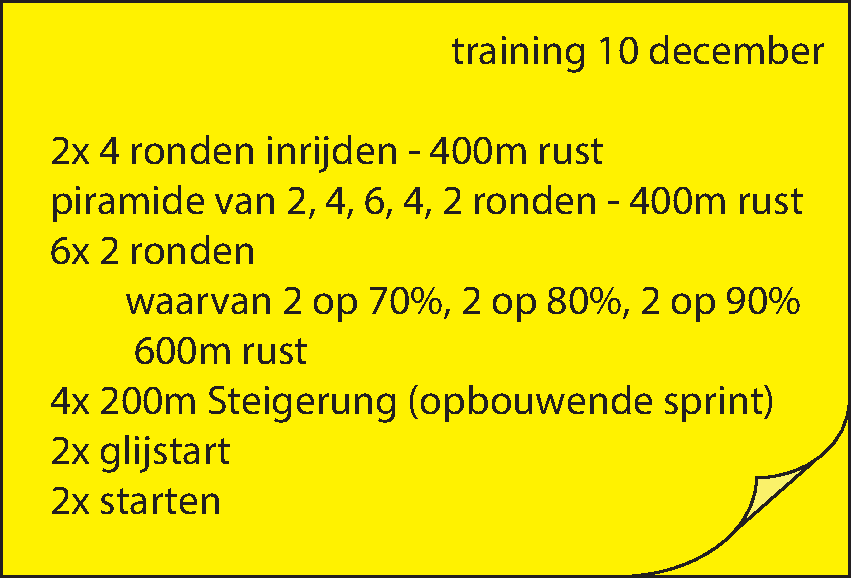
\includegraphics[width=0.4\textwidth]{style/images/training}
 \caption{Een typisch schaats-trainingsschema}
\end{wrapfigure}

Trainingen, bij bijvoorbeeld schaatsen, bestaan uit losse trainingsonderdelen. Allround schaatsers moeten bijvoorbeeld 4 ronden warmrijden, dan 6 keer 2 ronden sprinten, dan 4 keer een sprintje van 200 meter, 2 keer een glijstart en dan 2 keer een echte start bij de coach, vanuit de zijkant van de baan. Tussendoor is er rust, zo is het gebruikelijk om na een opdracht tenminste 400 meter uit te glijden. Het verschil tussen training en rust is af te leiden uit de verhouding tot de maximale snelheid.

Veel trainingselementen bestaan dus uit korte opdrachten, waar het juist om snelheid gaat. Een enkele lus is dan niet afdoende, omdat de rust voor of na de opdracht mee wordt gewogen. Sporters starten en stoppen namelijk niet precies boven de lus, maar starten vaak na de bocht en stoppen afhankelijk van de afstand van de opdracht op een willekeurig punt. 

Andere trainingen van bijvoorbeeld lange afstands- of marathonschaatsers kunnen bestaan uit één element: de hele training lang schaatsen, zonder overeind te komen. Wanneer er op tactische punten detectie-lussen geïnstalleerd zijn, is er bijvoorbeeld ook onderscheid te maken tussen bochten en de rechte stukken. Bij sporten met een ronde baan verschilt de snelheid in de bocht namelijk erg met die op het rechte eind. Deze vergelijking gebeurt nu al in Thialf, in het professionele circuit tijdens wedstrijden op televisie.

Topsporters zijn enorm prestatiegericht en als je al aan de top zit, dan kunnen kleine aanpassingen aan je techniek, ademhaling et cetera, grote verschillen maken. Coaches van professionele teams houden zich daarom bezig met allerhande analyses. Naast ademanalyse en hartslag monitoring, is het in Thialf bijvoorbeeld ook mogelijk om (van maximaal 20 schaatsers) continu de positie te bepalen met een in-door positioning system (IPS) ontwikkeld door InnoSportLab\footnote{\url{http://www.innosportlabthialf.nl}}.

Al deze geavanceerde analyses zijn echter te duur en kosten te veel tijd voor recreatieve sporters. MyLaps X2 biedt in combinatie met ons eindproduct recreatieve sporters toch een manier om analyses uit te voeren en zich naar een hoger niveau te tillen.

\section*{Opbouw Verslag}

In dit verslag zal allereerst in hoofdstuk~\ref{ch:opdracht-en-omschrijving} de opdracht en het domein van de opdracht worden toegelicht. Vervolgens zal in hoofdstuk~\ref{ch:project-methodologie} de methodologie worden behandeld die tijdens het proces is aangehouden. Hierna zal in hoofdstuk~\ref{ch:systeem-ontwerp-en-implementatie} gedetaileerd worden toegelicht op welke manier het systeem is ontworpen, welke implementatiekeuzes er zijn gemaakt en hoe deze keuzes zijn uitgewerkt. In hoofdstuk~\ref{ch:evaluatie} wordt behandeld hoe de applicatie wordt geëvalueerd met behulp van tests en feedback van verschillende betrokken partijen en mogelijke eindgebruikers. Ten slotte zal in hoofdstuk~\ref{ch:discussie} onder andere worden besproken in hoeverre het project een succes is geweest, wat er moet gebeuren om ook een Android applicatie te kunnen maken en welke invloed bepaalde keuzes hebben gehad op het project. Tenslotte zal in de conclusie, in hoofdstuk~\ref{ch:conclusie} worden aangegeven hoe de applicatie is opgeleverd, zal er een visie gegeven worden op de doorontwikkeling van de applicatie en zal worden besproken welke toekomst wij zien voor de applicatie.

\chapter{Opdracht en Omschrijving} \label{ch:opdracht-en-omschrijving} Emando B.V. is een jong bedrijf dat maatwerksoftware maakt. Momenteel ontwikkelt Emando voor de \acf{KNSB} een nieuw licentie-aankoop- en -beheersysteem, een nieuw wedstrijdadministratiesysteem en een nieuwe schaatstijdendatabase. Naar aanleiding van eerder contact met de \ac{KNSB} over toegang tot de schaatstijdendatabase zijn wij in telefonisch contact gekomen met Johan Stokking van Emando. Tijdens het oriënterende gesprek bleek dat zowel wij als Emando er geïnteresseerd in waren dat wij ons Bachelor Eindproject bij Emando zouden uitvoeren, onder begeleiding van de heer Stokking.

\section{Opdrachtsamenvatting}
In de weken voorafgaand aan het Bachelor Eindproject is in samenspraak met Emando de opdrachtomschrijving gemaakt. Bij het brainstormen zijn de minimale eisen en de mogelijke extra functies bedacht:

\begin{quotation}
\itshape
Het ontwerpen en ontwikkelen van een systeem voor het weergeven en analyseren van (live) recreatieve en trainingsdata in de context van baansporten (bijvoorbeeld schaatsen en baanwielrennen). Dit systeem zal realtime gegevens van de baan, maar ook opgeslagen gegevens uit het verleden, inzichtelijk maken voor sporters, coaches en eventuele toeschouwers (volgers). Daarnaast zal er de mogelijkheid zijn om een sociale component en een competitie element toe te voegen, en een mogelijkheid om aggregatie op data uit te voeren.

Het systeem ondersteunt het sporten: sporters hoeven hun training niet te onderbreken, doordat audio-cue's en sport-specifieke schermen geïmplementeerd worden. De sociale component bestaat uit het volgen van vrienden (mede-sporters) en het delen van resultaten. Het competitie element zal een virtuele competitie tussen vrienden omvatten.

Technisch gezien zal er een scheiding gemaakt worden tussen de diverse toepassingen (clients) en de API. De API biedt toegang tot realtime data en de diverse modulaire (sport-specifieke) aggregaties, waarbij de mogelijkheid bestaat voor bijvoorbeeld coaches om te abonneren op meerdere sporters. De API zal gekoppeld worden op bestaande systemen die data van transponders ontsluiten.
\end{quotation}

Om richting te geven aan het toekomstige applicatie, is de opdrachtomschrijving ambitieus opgesteld. We hebben vanaf het begin de instelling gehad om eerst een minimale versie te maken die werkt, om vervolgens de eerste versie uit te bouwen tot een volwaardige applicatie.

Zoals te lezen is in de opdracht zal er zowel een mobiele applicatie als een back-end systeem ontwikkeld worden. In sectie \ref{sec:programma-van-eisen} worden de elementen uit de opdrachtomschrijving uitgesplitst en omgezet in functionaliteiten met de bijbehorende prioriteit.

\section{Doelgroep en Gebruikers}

\newcommand{\doelgroep}{}
\label{sec:doelgroep}

\subsection{Schaatsers}
De voornaamste doelgroep van onze applicatie zijn de recreatieve en amateur schaatsers. Zij moeten met behulp van onze applicatie meer inzicht krijgen in hun prestaties en trainingen. 
Om er voor te zorgen dat deze groep gebruikers onze applicatie verkiest boven de reeds bestaande (minder uitgebreide) systemen, dienen zij snel en gemakkelijk met de applicatie aan de slag te kunnen gaan.
Bij een té ingewikkeld systeem zullen zij afhaken en de overstap naar onze applicatie wellicht niet willen maken.
Omdat zij de belangrijkste doelgroep zijn van de applicatie, is het belangrijk dat zij gemotiveerd worden om de applicatie te blijven gebruiken en hen tevens motiveren om ook anderen aan te sporen dit te doen.
Met behulp van sociale componenten zoals trainingsgroepen, het volgen van andere schaatsers en leaderboards kan onze applicatie hen hierin stimuleren.
\subsection{Coaches}
Als tweede doelgroep zijn er de coaches van de schaatsers. Dit zijn mensen die de schaatsers begeleiden bij hun trainingen en wedstrijden. Zij beschikken zelf niet altijd over een transponder, omdat niet iedere coach zelf schaatst.
Zij willen graag snel en gemakkelijk inzicht in de data van de schaatsers die zij coachen. Het moet voor hen dus gemakkelijk zijn om snel tussen schaatsers te kunnen switchen en deze prestaties zowel onderling als per training gemakkelijk te kunnen vergelijken.
\subsection{Overige gebruikers}
Tot slot is er de groep gebruikers die zelf geen deel uitmaakt van de schaatswereld. Zij zijn geen schaatsers of coaches en zijn met name geïnteresseerd in de mogelijkheden van de applicatie en het volgen van kennissen of bekende schaatsersn.
Ook zij moeten in staat zijn om de applicatie gebruiken, weliswaar in mindere mate.

\section{Reeds bestaande vergelijkbare systemen}

\newcommand{\vergelijkbaresystemen}{}
\label{sec:vergelijkbare-systemen}

Er bestaan al enkele oplossingen die functionaliteit bieden die vergelijkbaar is met die van de applicatie die wij gaan bouwen. Strava (figuur~\ref{fig:strava}) en RunKeeper (figuur~\ref{fig:runkeeper}) maken gebruik van GPS om onder andere hardlopers en wielrenners van realtime informatie te voorzien. \mylaps Practice (figuur~\ref{fig:mylapspractice}) is een website waar je na je training je prestaties kan terugkijken. Er bestaat ook een iPhone App voor \mylaps Practice (figuur~\ref{fig:mylapspractice-app}). Coach Watch (figuur~\ref{fig:coachwatch}) is een iPad applicatie waarmee coaches hun teams kunnen volgen.

\begin{figure}[ht]
\centering
\subfigure[Strava]{
    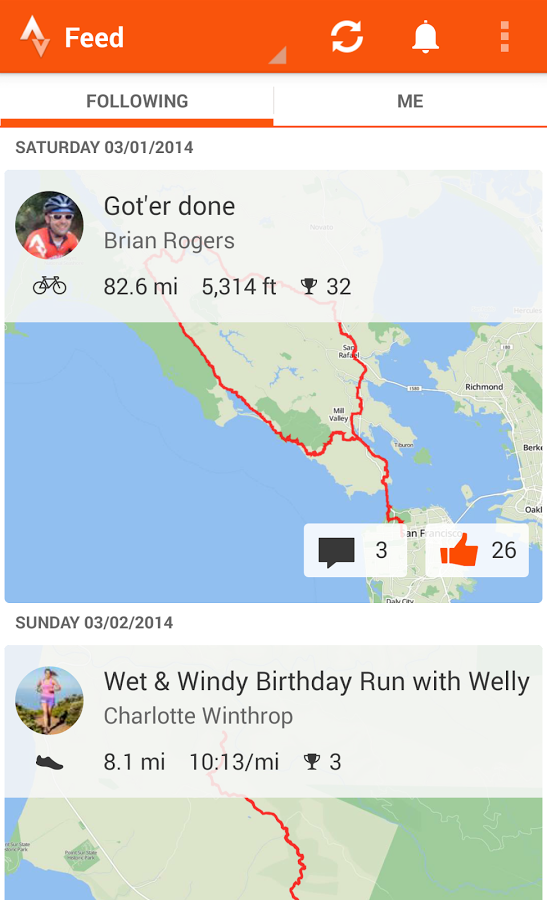
\includegraphics[height=5cm]{style/images/Strava}
    \label{fig:strava}
}
\subfigure[RunKeeper]{
    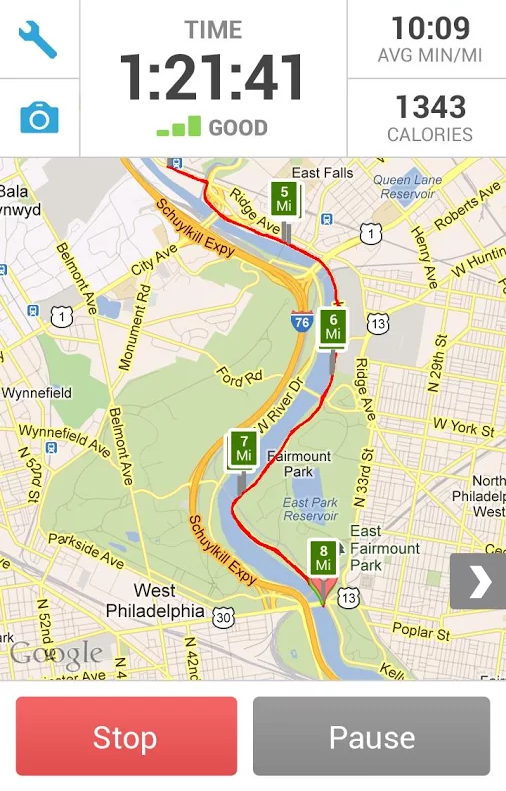
\includegraphics[height=5cm]{style/images/RunKeeper}
    \label{fig:runkeeper}
}
\subfigure[Coach Watch]{
    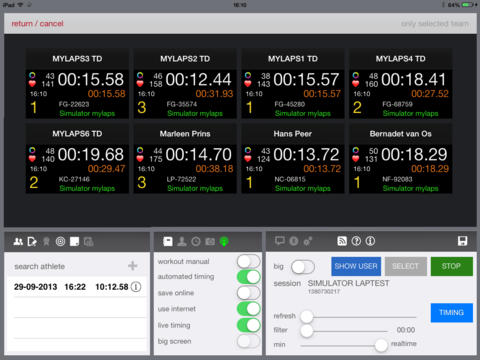
\includegraphics[height=5cm]{style/images/CoachWatch}
    \label{fig:coachwatch}
}

\subfigure[\mylaps Practice]{
    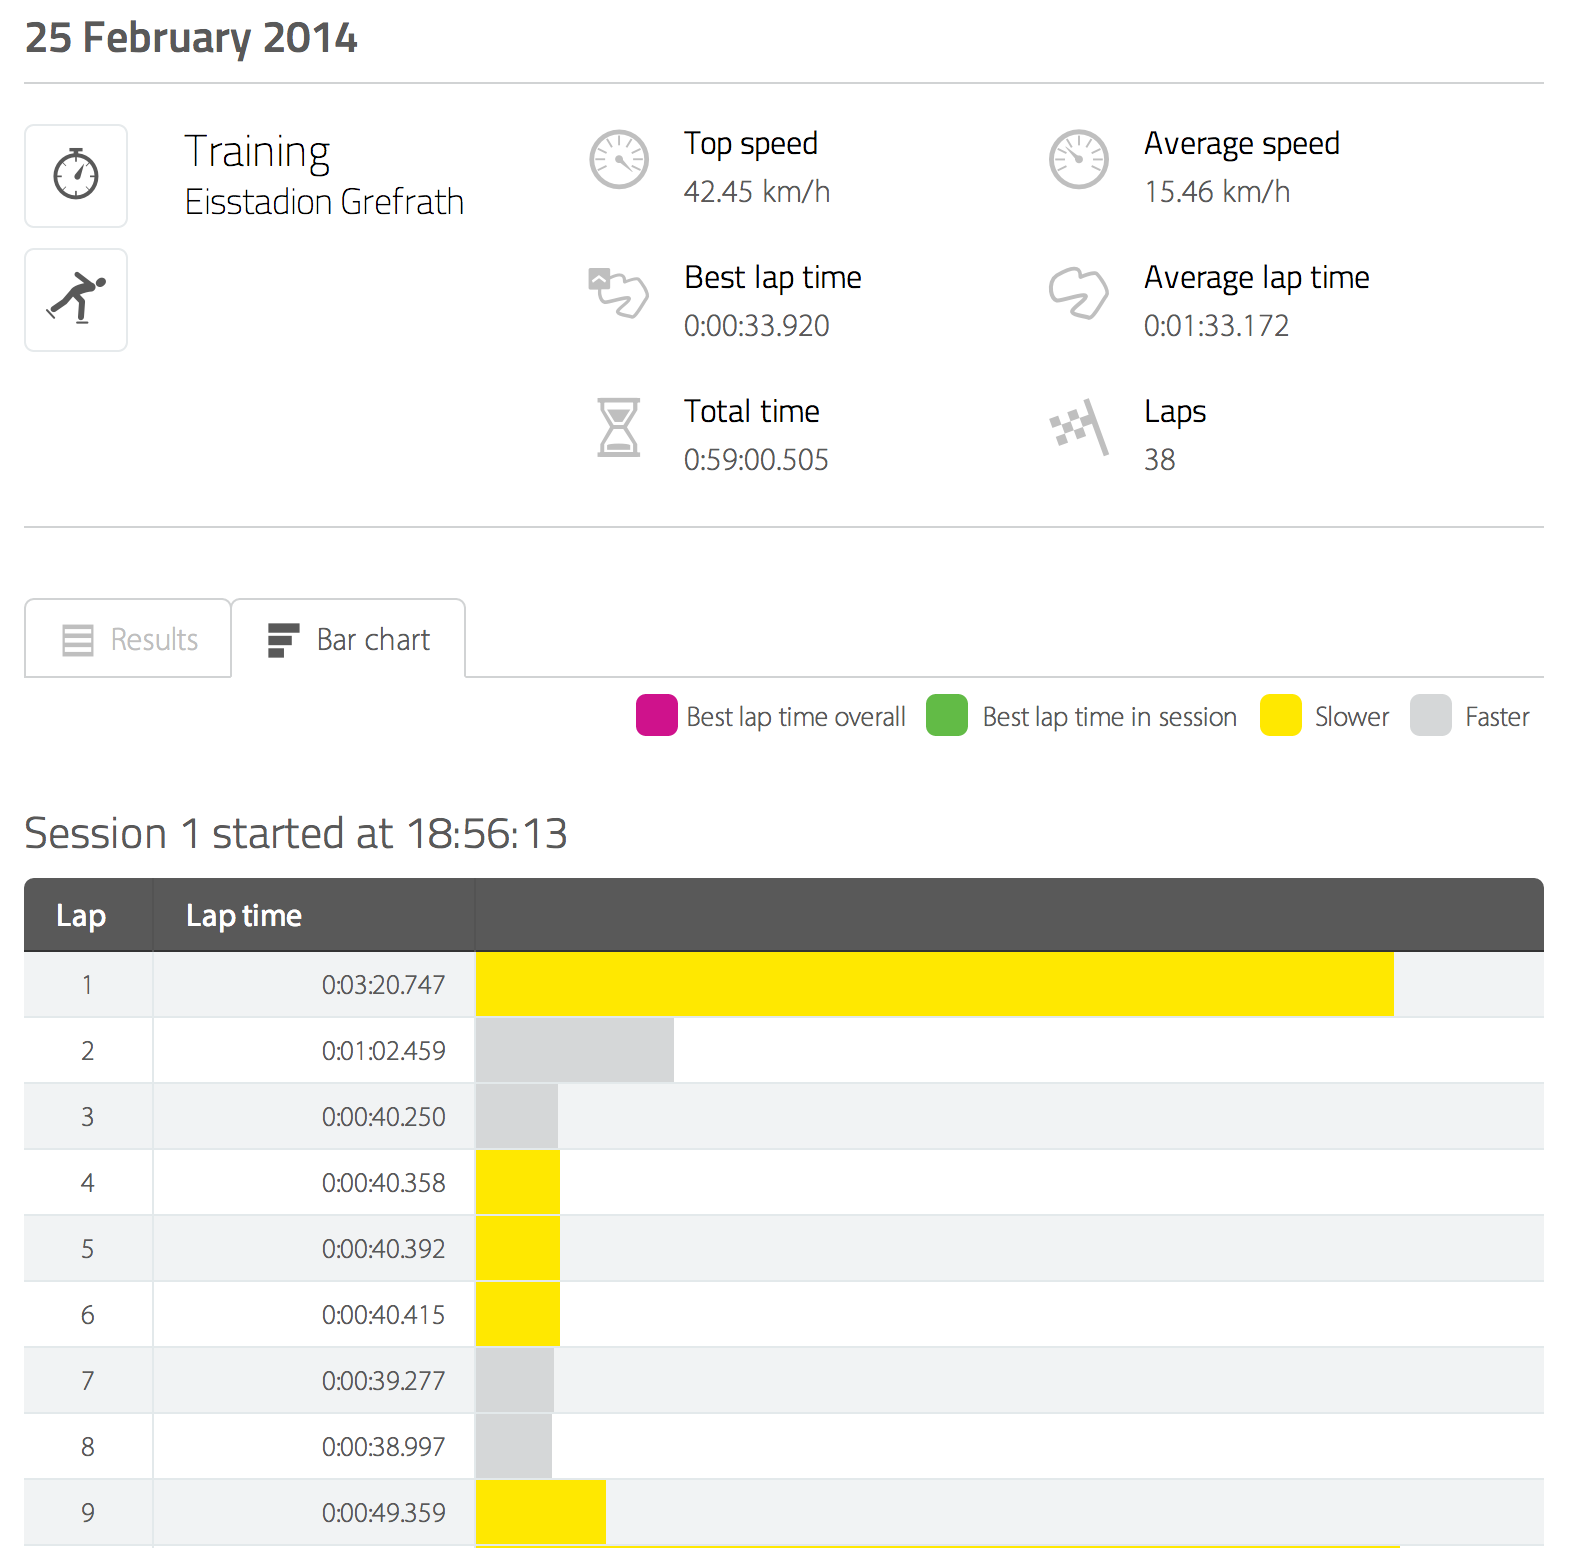
\includegraphics[height=7cm]{style/images/MyLapsPractice}
    \label{fig:mylapspractice}
}
\subfigure[\mylaps Practice App]{
    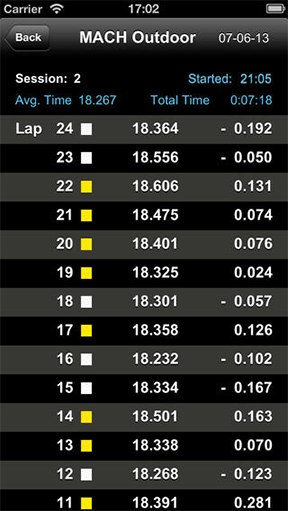
\includegraphics[height=7cm]{style/images/MyLapsPractice-App}
    \label{fig:mylapspractice-app}
}

\caption{Soortgelijke oplossingen}
\label{fig:soortgelijke-oplossingen}
\end{figure}

Strava en RunKeeper zijn voor baansporten, zoals bijvoorbeeld schaatsen, niet goed bruikbaar, aangezien GPS op de banen slecht presteert, waardoor de informatie niet nauwkeurig genoeg is. \mylaps Practice en Coach Watch maken wel gebruik van de detectielussen in de banen. De \mylaps Practice website kan alleen gebruikt worden voor het achteraf bekijken van sportprestaties en deze de applicatie is vooral gericht op motorsporten. CoachWatch is een (vrij dure) applicatie die vooral gericht is op coaches en dus minder geschikt voor trainingen of voor amateurschaatsers.

Emando ziet de mogelijkheid om een applicatie te bieden die gebruikmaakt van de detectielussen in de banen, die live gegevens kan tonen op een smartphone en die ook nog eens goedkoop of gratis is. Onze applicatie richt zich dus op het invullen van de stukken die missen in de bestaande oplossingen.
    
    % systemen in ontwikkeling bij Emando
\section{Programma van eisen} % MoSCoW shizzle

\newcommand{\programmavaneisen}{}
\label{sec:programma-van-eisen}

Traditioneel gezien wordt bij software ontwikkeling het MoSCoW model gebruikt. Het MoSCoW model onderscheid functionaliteiten op basis van prioriteiten. De verschillende niveau's zijn must-, should-, could- en won't-haves. De vertaling van deze niveau's spreekt voor zich.

Wij gebruiken het in combinatie met SCRUM veel gebruikte \acf{mvp} model. Hierbij wordt gedefinieerd wat het product minimaal moet kunnen om bruikbaar te zijn. In die zin komt onze \ac{mvp} dus overeen met de must-haves uit het MoSCoW model. Eventuele tegenslagen mogen er niet toe lijden dat het \ac{mvp} niet gemaakt wordt, daarom is de planning om het \ac{mvp} al in de 4e week af te hebben. Gebruikers kunnen op dat moment met de applicatie spelen en de kern-functionaliteit beoordelen.

Het \ac{mvp} biedt op zich zelf nog niet alle features die zowel wij als de opdrachtgever graag geïmplementeerd zouden willen zien. Het eindproduct zal over enkele bijzondere functies moeten beschikken, de zogenaamde `killer-features' om het product populair te maken. Deze features zijn in die zin dus vergelijkbaar met de should-haves uit het MoSCoW model.

Na het \ac{mvp} en de features die het verschil maken zijn er ook nog een aantal features die niet noodzakelijk zijn en geen groot verschil zouden maken. Deze features zijn te vergelijken met could-haves uit het MoSCoW model. We zullen zeker niet alle could-haves implementeren, en wellicht komen enkele should-features ook niet aan bod. Wellicht volgt uit een user study dat de door ons bedachte could-haves door users erg gewenste features zijn. In overleg met onze begeleiders kunnen we besluiten deze features te implementeren. Bovendien bieden de could-haves een goede leidraad bij toekomstige ontwikkeling na afloop van ons project.

\subsubsection{Must-haves (\ac{mvp})}

\begin{itemize} \parskip0pt \parsep0pt
    \item Bruikbaar als applicatie op smartphone(s)
    \item Architectuur is sport-agnostisch
    \item De sport-specifieke weergave van tijden is voor schaatsbanen geïmplementeerd
    \item Mogelijkheid om een account aan te maken
    \item Real-time transponder doorkomsten tonen van geselecteerde sporters
    \item Historische doorkomsten van een persoon, gegroepeerd per dag of training
    \item De voor bovenstaande features ontwikkelde API, moet het mogelijk maken om de API uit te breiden en de applicatie aan te passen.
\end{itemize}

\subsubsection{Should-haves}

\begin{itemize} \parskip0pt \parsep0pt
    \item Mogelijkheid om account te koppelen aan Facebook
    \begin{itemize}
        \item Mogelijkheid om prestaties en records te delen op Facebook
    \end{itemize}
    \item Audio-cues geven aan sporter over doorkomsten van een geselecteerde transponder
    \item Leaderboards tonen met sporters gerangschikt naar prestaties en disciplines (virtuele competitie), zoals:
    \begin{itemize}
        \item rondetijd (actuele/gemiddelde/snelste)
        \item snelheid (gemiddelde/snelste)
        \item cumulatieve afstand (per seizoen/week/training)
        \item rust/intensief-ratio (hoeveelheid rondjes, ratio)
        \item achievements-punten (verbeter jezelf 10\%, voor 7 uur op de baan, 2 trainingen per week)
    \end{itemize}
    
    \item Groepen-functionaliteit \begin{itemize}
        \item Mogelijkheid om een lege groep te maken
        \item Mogelijkheid om sporters uit te nodigen voor een groep
        \item Mogelijkheid om op uitnodiging in een groep te gaan
        \item Mogelijkheid om uit een groep te gaan
    \end{itemize}

    \item Zowel leaderboards als real-time doorkomst-schermen kunnen worden gefilterd op groep of baan
     
    \item Privacy instellingen bieden aan gebruikers
    \begin{itemize}
        \item Mogelijkheid om een account publiekelijk of anoniem te laten indexeren
        \item Mogelijkheid om eigen data te delen met anderen
    \end{itemize}

\end{itemize}

\subsubsection{Could-haves}

\begin{itemize} \parskip0pt \parsep0pt
    \item Suggesties krijgen om met soortgelijke schaatsers te gaan schaatsen
    \item Training kunnen exporteren naar RunKeeper\footnote{Fitness logboek platform, \url{http://www.runkeeper.com}}
\end{itemize}

\subsubsection{Won't-haves}

Het door Emando ontwikkelde systeem Vantage zal de huidige systemen voor wedstrijduitslagen vervangen. Koppelingen op het huidige systeem zouden dus snel niet meer werken en het nieuwe systeem is niet af tijdens ons project.
\begin{itemize} \parskip0pt \parsep0pt
    \item Wedstrijdloting en uitslagen bekijken
    \item Persoonlijke records tonen
\end{itemize}


\chapter{Projectmethodologie} \label{ch:project-methodologie} Emando zit in het BizSpark programma van Microsoft. Vanuit BizSpark kunnen alle ontwikkeltools gratis gebruikt worden en Emando leunt dan ook op Microsoft technologie. Onderstaande methodologieën kunnen eenvoudig geïntegreerd worden in de ontwikkelomgeving Visual Studio. We zullen niet afwijken van de methodologieën die Emando nu al gebruikt, omdat ons deze omgeving wordt aangeboden en om onderhoudbaarheid in de toekomst te garanderen.

\section{Scrum}
In overleg met de opdrachtgever is er gekozen voor een scrum aanpak voor het project. Scrum is een flexibele manier om software te ontwikkelen. Hierbij gaan we werken in een multidisciplinair team waarmee we in korte sprints, met een vaste lengte van 2 weken, werkende software opleveren en geleidelijk stabiele functionaliteit toe voegen. Een scrum aanpak heeft als voordeel dat na iedere sprint er een werkend product af is, waarna de eisen en doelstellingen gemakkelijk bijgesteld kunnen worden. Met scrum kunnen na de gebruikerstest, halverwege het project, de doelstellingen bijgesteld worden aan de hand van de uitkomst van deze test. Door deze agile methode toe te passen sluit het eindproduct altijd zo goed mogelijk aan op de wensen van de opdrachtgever en de end-users.

\section{Stand up meetings}
Om het overzicht binnen het project te waarborgen, zullen er iedere werkdag aan het begin van de dag stand up meetings met alle projectleden plaatsvinden. Bij deze stand up meetings wordt kort besproken waar momenteel aan gewerkt wordt, in hoeverre dit nog op schema ligt en waar de uitdagingen liggen voor de komende dagen. De opdrachtgever zal minstens twee keer per week aanwezig zijn bij deze meetings, hetgeen naar wens vanzelfsprekend vaker kan.

\section{\acl{tfs}}
Emando gebruikt \ac{tfs} voor het versiebeheer van broncode, het bijhouden van het ontwikkelproces, het tracken van issues en het visualiseren van de voortgang in projecten. De gemakkelijke integratie van \ac{tfs} met Visual Studio zorgt ervoor dat issues en backlog items gemakkelijk toegewezen kunnen worden aan developers, waarna zij deze kunnen openen en hiermee aan de slag kunnen binnen hun IDE. De status van deze items kan zowel vanuit de IDE als online aangepast worden en bij het afvinken van items kunnen deze gekoppeld worden aan versie nummers, zodat deze achteraf makkelijk vindbaar zijn.
Ook zorgt de visualisatie van de zogenaamde ‘burndown’ van het project voor een inzichtelijke manier, waarbij de opdrachtgever in een handomslag de voortgang van het project in kan zien. Daarnaast biedt \ac{tfs} inzicht in de tijd die ieder issue en backlog item kost, hetgeen een goede indicatie is voor de scrum sprint.

\subsection{Verantwoordelijkheden}

{\par \bigskip \par \color{red} TODO: Backlog Verantwoordelijke \par \bigskip \par }

\subsection{Taakverdeling}

{\par \bigskip \par \color{red} TODO: Verdeling van Tasks \par \bigskip \par }

Verdeling van Tasks (vaak: patty back-end, hylke gui \& test, herman app)

\section{Code Reviews}

{\par \bigskip \par \color{red} TODO: Code Reviews \par \bigskip \par }

\section{Project keuzes}
Qua talen, frameworks en libraries moesten al vroeg enkele afwegingen gemaakt worden. Uiteindelijk hebben we gekozen om te werken met onder andere C\#, Xamarin en SignalR. De redenatie achter deze keuzes is te lezen in het orientatieverslag (sectie \ref{sec:orientatie-back-end}
en \ref{sec:orientatie-client}).



\chapter{Systeemontwerp en -implementatie} \label{ch:systeem-ontwerp-en-implementatie} \begin{wrapfigure}{r}{0.56\textwidth}
  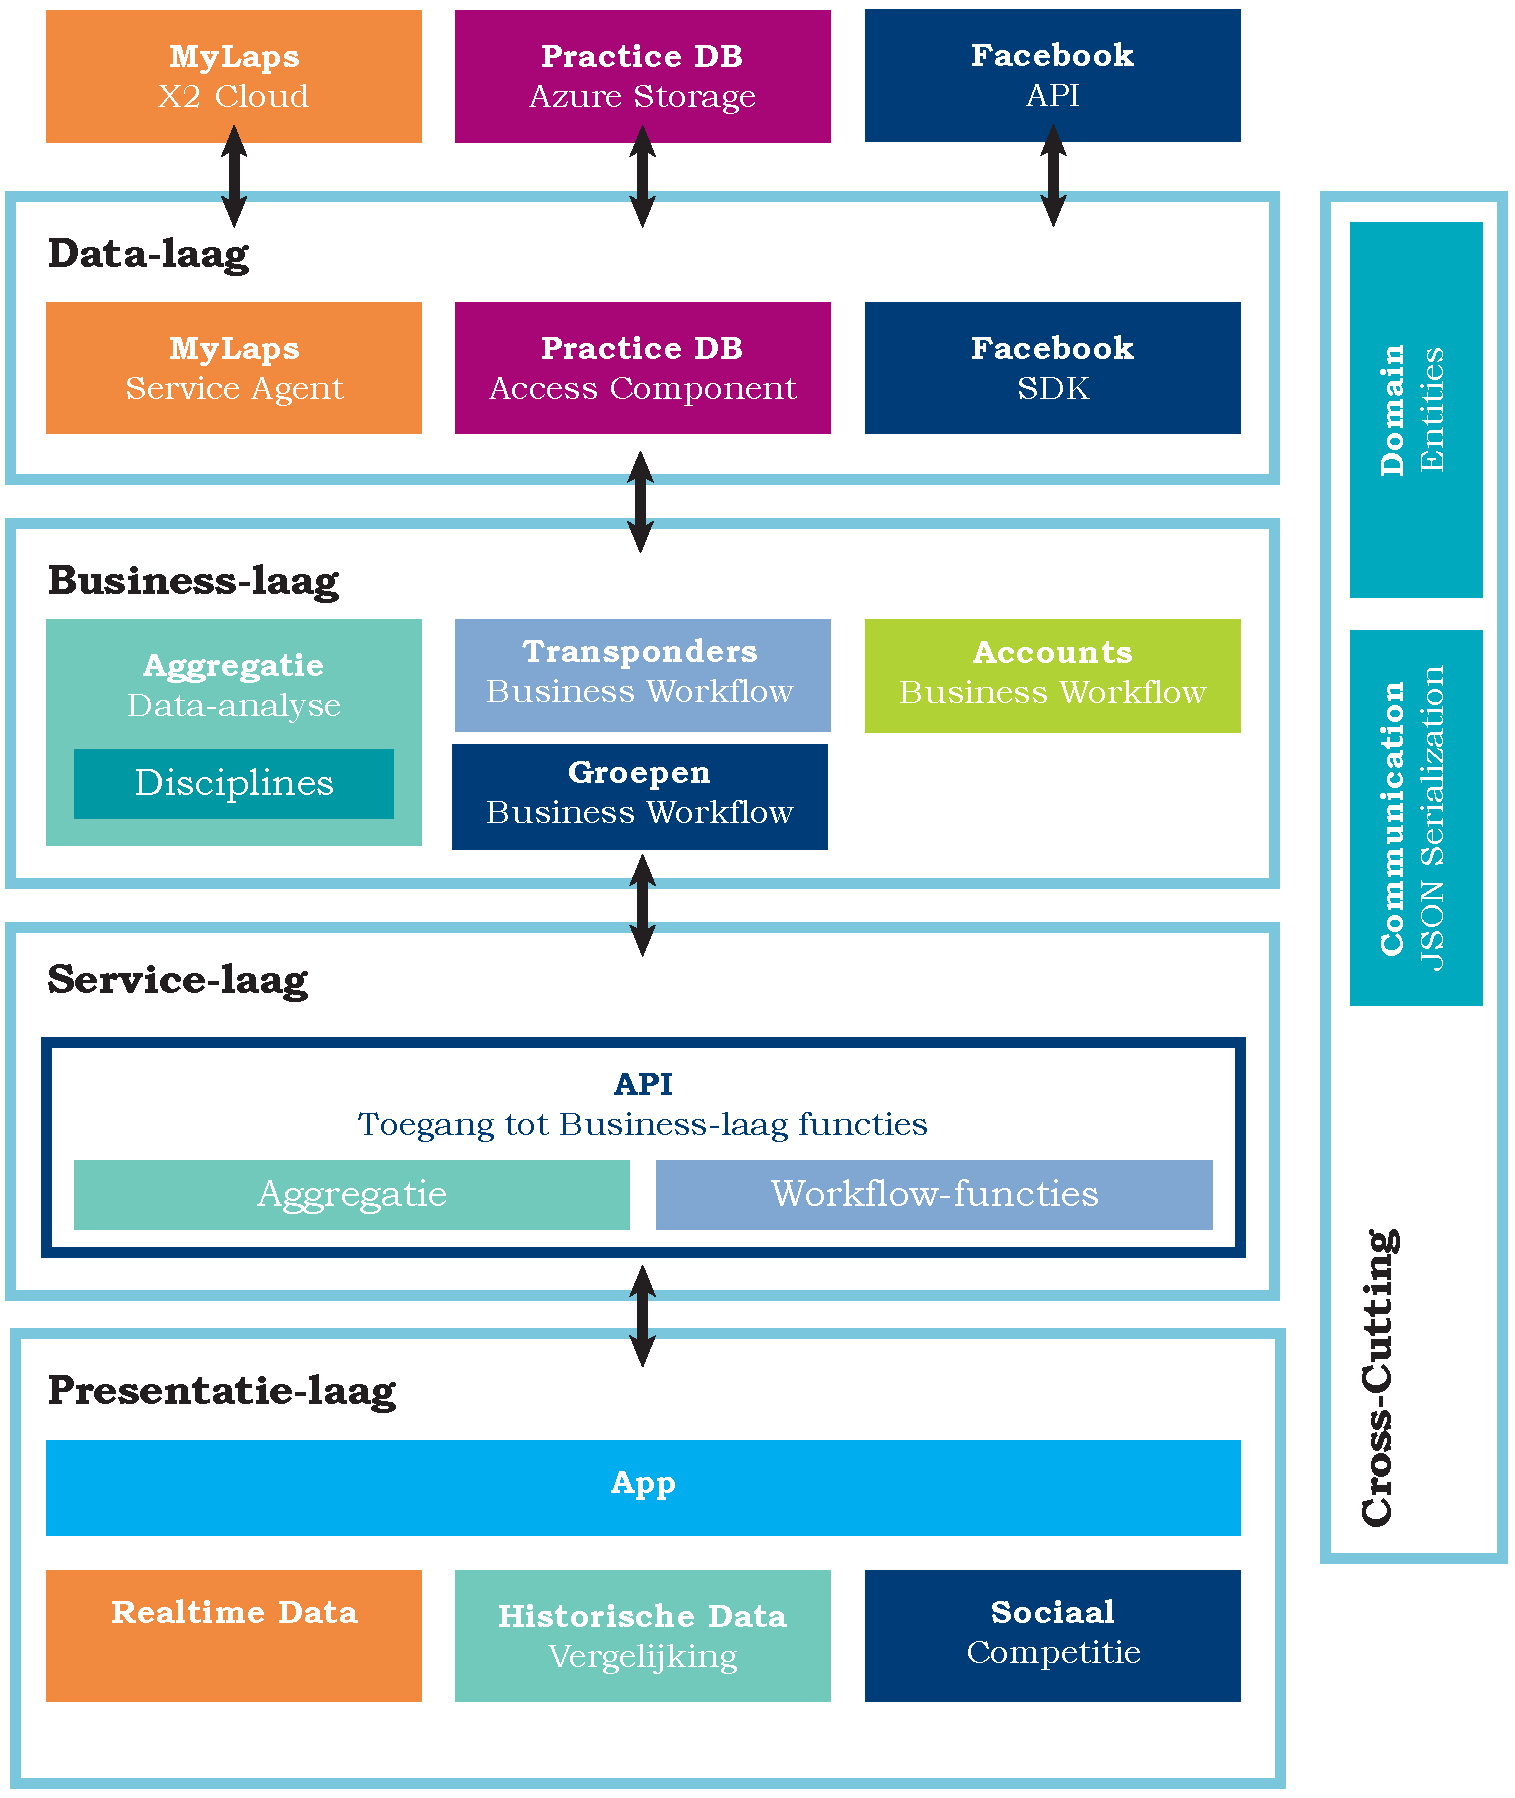
\includegraphics[width=0.6\textwidth]{style/images/Layers}
  \caption{Diagram van de lagen van de applicatie}
  \label{fig:diagram-layers}
\end{wrapfigure}

Zoals besproken tijdens de meeting van 23 april (Pagina \pageref{sec:meeting-23-apr}), worden applicaties die Emando ontwikkelt opgedeeld in vier lagen. Deze opzet zullen wij ook aanhouden.

\begin{description}
\item[De presentatielaag] verzorgt de weergave. De presentatielaag bevind zich in de code van de mobiele applicatie en bevat zowel platform onafhankelijke View-Models en hulpmiddelen als platform specifieke User Interface elementen.
\item[De servicelaag] is de interface tussen de server en de mobiele apps. Deze gebruikt de twee technieken SignalR en WebApi.
\item[De businesslaag] is verantwoordelijk voor het ophalen en verwerken van de data. Deze laag bevat een verbinding met de service- en datalaag. Met deze verbindingen is deze laag is staat met behulp van logica data op te halen, te verwerken, eventueel op te slaan en door te sturen naar de servicelaag. 
\item[De datalaag] is verantwoordelijk voor alle verschillende databronnen: Entity Framework, Table Storage en MyLaps. Deze laag bevat zelf geen verbindingen andere lagen, maar de data kan met behulp van repositories vanuit de business laag opgevraagd worden.

\end{description}

Naast deze vier lagen is er ook nog een deel van de code die gedeeld wordt door alle andere lagen: \textbf{``cross-cutting''}. In de cross-cutting laag bevinden zich voornamelijk de domein entiteiten, zodat alle server-lagen deze entiteiten kunnen gebruiken. Naast de entiteiten wordt ook de JSON serialisatie van de entiteiten in de cross-cutting laag geregeld: er zijn  speciale te serialiseren afgeleide modellen, met zo weinig afhankelijkheden van frameworks dat ze in een \ac{pcl} kunnen. Hierdoor kunnen de mobiele applicaties dezelfde modellen gebruiken als de servicelaag, en kunnen de modellen via de Websockets- en HTTP-verbinding van SignalR en WebAPI verstuurd worden. Deze entiteiten bevatten allen een context Id en user Id, welke aangeeft voor welke context (groep, baan of gebruiker) bedoelt is en van wie deze entiteit is. Op deze manier is SignalR in staat om deze entiteiten te versturen naar de juiste gebruikers.

  % 4 lagen
  % - presentatie laag
  % - service laag: API
  % - business laag: analyse en aggregatie
  % - data laag
  
\section{Datalaag}
De applicatie bevat data uit verschillende bronnen, en slaat zijn data in verschillende bronnen op. Deze data en de verbindingen met de bronnen vormen de datalaag.

\subsection{Ruwe inkomende data}

De transponderleverancier MYLAPS heeft een SDK beschikbaar gesteld aan Emando, waarmee het mogelijk is om de doorkomsten van transponders realtime binnen te krijgen. Om deze databron te benaderen bevat de datalaag een Data Collector, geïmplementeerd als Azure Cloud Worker Role, welke non-stop draait op één cloud instance. Dit proces onderhoudt de verbinding met de MYLAPS SDK.

Vanuit de MyLAPS SDK ontvangt de data laag realtime de doorkomsten van iedere transponder die langs een lus komt. Deze doorkomsten bevatten een tijdstip, een transponder nummer en een plaats op de baan. Zodra een van deze doorkomsten binnen komt, wordt deze direct opgeslagen voor toekomstig gebruik in een doorkomsten tabel in Azure Table Storage. Het kan namelijk voorkomen dat er op dit moment geen gebruiker van onze applicatie is, welke zijn transponder nummer heeft gekoppeld aan zijn account. Wanneer dit het geval is, kunnen er (nog) geen aggregaties uitgevoerd worden op deze data.

\begin{figure}[ht]
  \begin{center}
  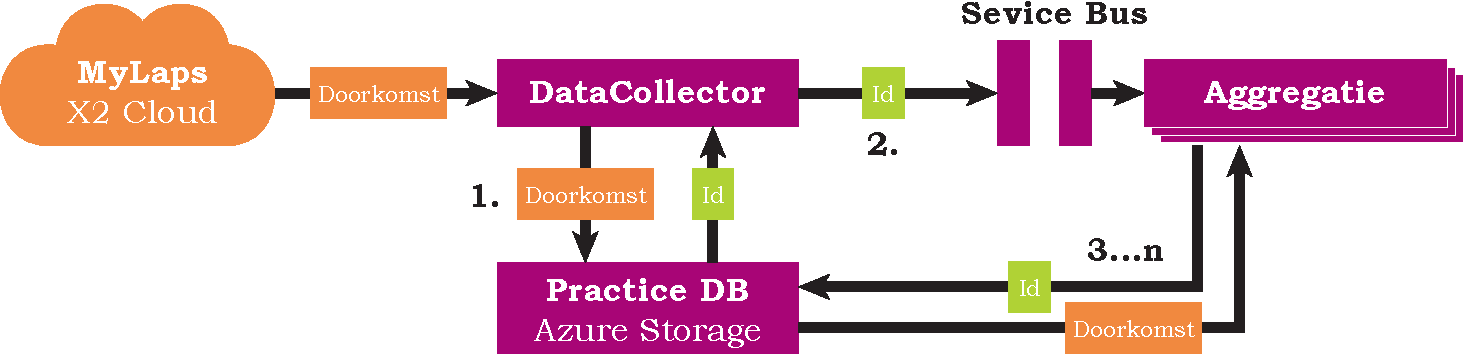
\includegraphics[width=\textwidth]{style/images/datacollector-flow}    
  \end{center}
  \caption{De werking van de Data Collector en de Service Bus}
  \label{fig:datacollector}
\end{figure}

Door deze data op te slaan, is het mogelijk om later functionaliteit in te bouwen om alsnog over deze data te kunnen aggregeren.

Nadat de data opgeslagen is, wordt via een Azure Service Bus het Id van de doorkomst doorgestuurt naar het aggregatie process in de businesslaag. Het aggregatie process raadpleegt bij het binnenkrijgen van dit Id opnieuw de doorkomst, om zo minder data over de service bus te versturen en altijd over up to date data te beschikken. Dit process wordt weergegeven in figuur~\ref{fig:datacollector}.

\subsection{Entiteiten}
In Figuur~\ref{fig:entiteiten} wordt een deel van de entiteiten die de applicatie gebruikt getoond, inclusief de onderlinge relaties. De entiteiten die te maken hebben met {\bfseries\color{tudelft-dark-blue} externe data} en {\bfseries\color{tudelft-green} accounts} worden opgeslagen met behulp van Azure SQL, zoals ook besproken in sectie~\ref{sec:database} van het oriëntatieverslag. De entiteiten die te maken hebben met {\bfseries\color{tudelft-orange} passings} en {\bfseries\color{tudelft-warm-purple} aggregaties} worden opgeslagen in Azure Table Storage.

\begin{figure}[ht]
  \begin{center}
  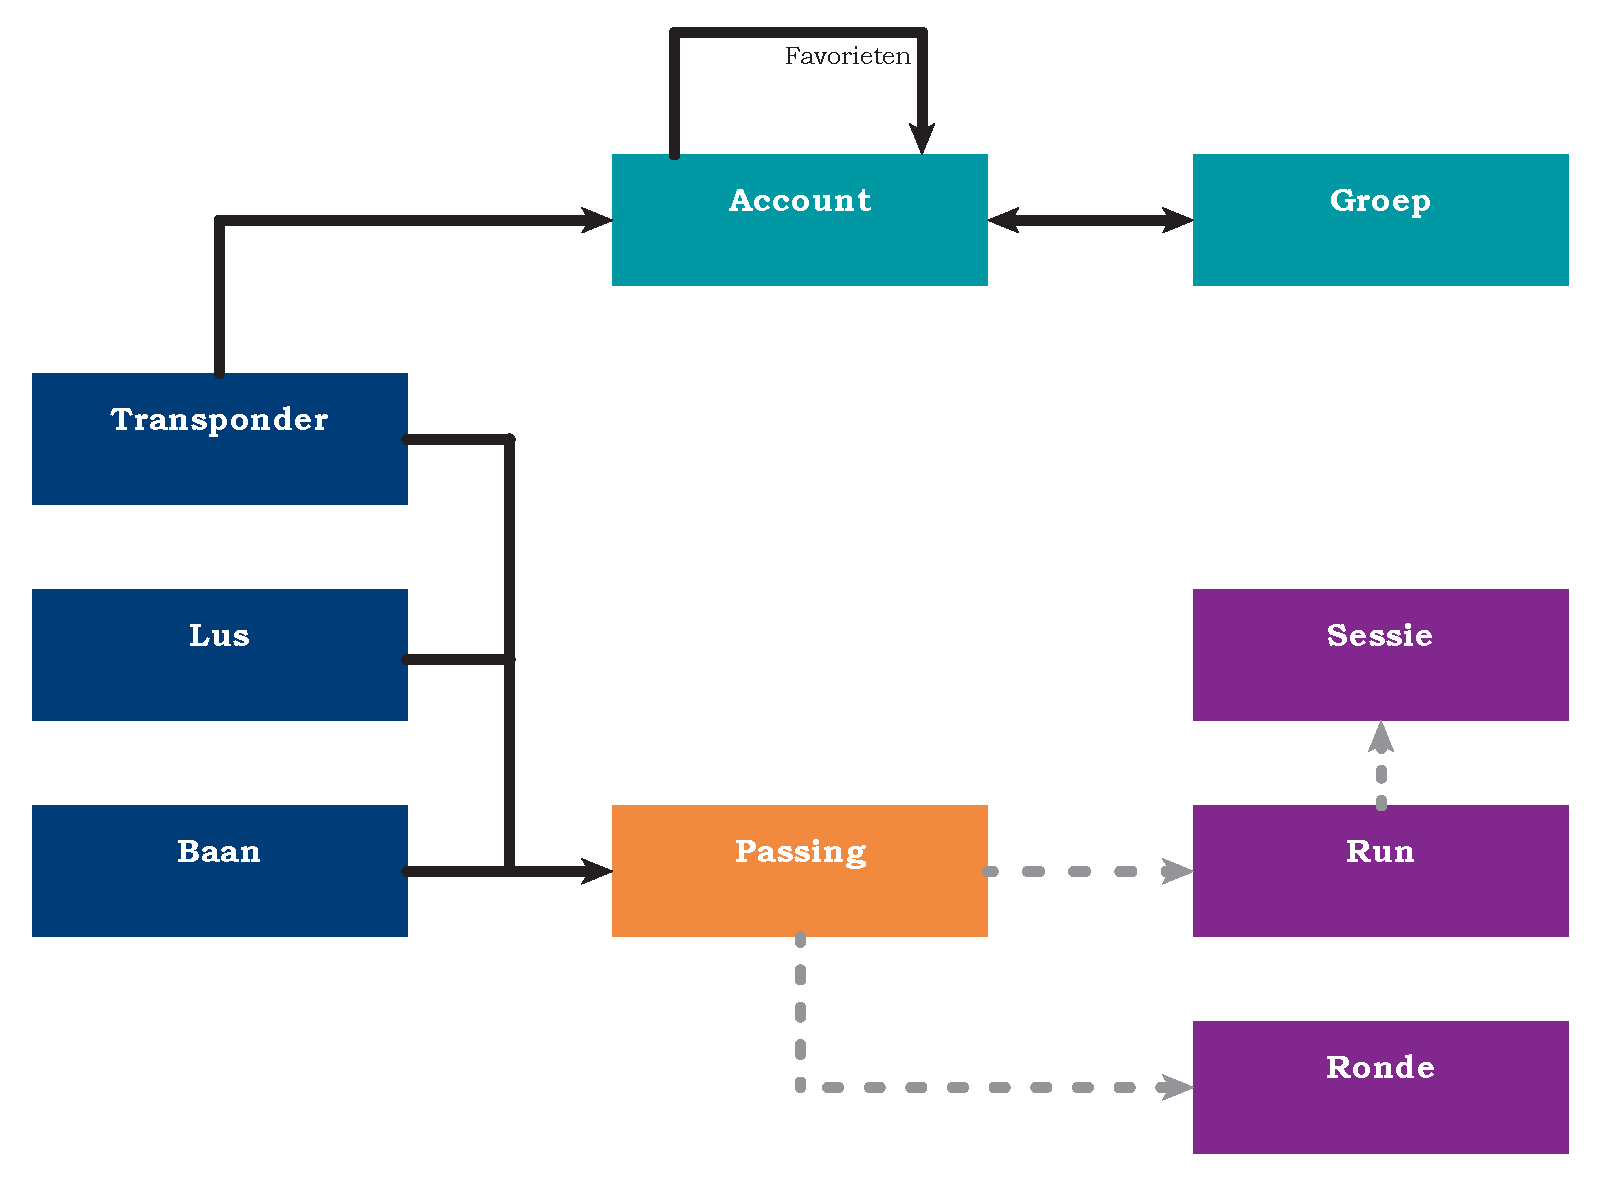
\includegraphics[width=.6\textwidth]{style/images/Entiteiten}    
  \end{center}
  \caption{De entiteiten en hun relaties.}
  \label{fig:entiteiten}
\end{figure}

Hoewel de daadwerkelijke structuur van de data in Azure Table Storage anders is dan in de figuur, geeft de figuur toch een goed beeld van deze entiteiten en hun relaties. 

\subsection{Azure SQL \& Entity Framework}
Azure SQL is de relationele SQL database van Azure en omdat de relaties in onze entiteiten worden beschreven door het Entity Framework~\cite{entityframework-msdn, entityframework-facto}, gebruikt onze applicatie de Entity Framework driver voor Azure SQL. Entity Framework is de defacto standaard voor relationele datalagen in ASP.NET. Het kan bijvoorbeeld relaties tussen entiteiten automatisch opzoeken. Ook hoeft er geen SQL code geschreven te worden, maar kan platformonafhankelijke LINQ code geschreven worden om entiteiten op te halen.

\subsection{Azure Table Storage}
De geaggregeerde data kan plat worden opgeslagen met behulp van NoSQL. Dit komt doordat alleen passings (doorkomsten), rondes en leaderboard-waarden entiteiten zijn in de aggregatie database. Zowel de sessie als het zijn van run of dan wel rust zijn eigenschappen van een ronde. De snelheid en segmenten worden niet opgeslagen.

Vanuit Emando ging de voorkeur voor het opslaan van de geaggregeerde data  uit naar de NoSQL Azure Table Storage. De Table Storage integreert eenvoudig met de reeds bestaande infrastructuur van het bedrijf. Bovendien biedt een gepartitioneerde en gesorteerde Table Storage tabel een groot performance voordeel: het goedkoop en snel kunnen selecteren van de laatste entiteiten per context.

Vanuit de Data Collector worden de doorkomsten die realtime binnen komen opgeslagen in Table Storage als backup. De structuur van deze tabel is terug te vinden in {\color{red} ref en tabel toevoegen }. Verderop in het aggregatieproces worden deze doorkomsten gekoppeld aan gebruikers. Deze aggregaties worden vervolgens opgeslagen in een aparte tabel binnen Azure Table Storage. De structuur van deze tabel is terug te vinden in {\color{red} ref en tabel toevoegen }.

Van snelheden, rondes, run/rust periodes en sessies worden leaderboards bijgehouden in Azure Table Storage. Deze hebben allen een eigen corresponderende tabel, zodat aggregaties parallel aan elkaar leaderboards kunnen updaten {\color{red} ref aggregatielaag }.
Alle leaderboards zijn voorzien van een leaderboard Id en een user Id. Het leaderboard Id houdt bij voor welke context het leaderboard geldig is. Dit kunnen banen, groepen, maar ook gebruikers zijn. Wanneer een gebruiker een ronde rijdt op een baan X, moeten zijn records voor de baan, zijn groepen en zijn eigen totalen geüpdatet worden. 

\begin{figure}[ht]
  \begin{center}
  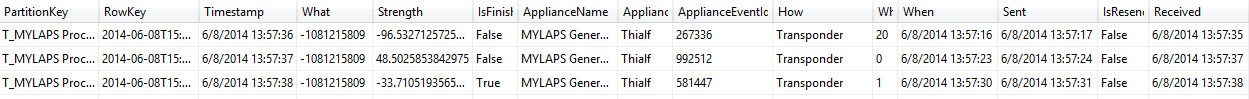
\includegraphics[width=.6\textwidth]{style/images/passingsStructure}    
  \end{center}
  \caption{De doorkomsten tabel met voorbeeld records. Hierbij is de Partition Key het type trasponder + transponder nummer en de Row Key het tijdstip waarop de doorkomst binnen kwam.}
  \label{fig:passingTableStructure}
\end{figure}

\begin{figure}[ht]
  \begin{center}
  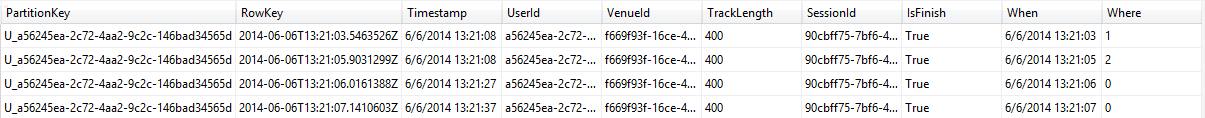
\includegraphics[width=.6\textwidth]{style/images/userPassingsStructure}    
  \end{center}
  \caption{De doorkomsten tabel met voorbeeld records. Hierbij is de Partition Key het account Id met een prefix voor gebruikers en de Row Key het tijdstip waarop de doorkomst binnen kwam.}
  \label{fig:userPassingTableStructure}
\end{figure}

\begin{figure}[ht]
  \begin{center}
  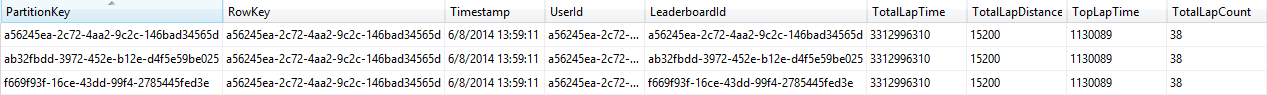
\includegraphics[width=.6\textwidth]{style/images/lapLeaderboardStructure}    
  \end{center}
  \caption{De ronde tabel met voorbeeld records. Hierbij is de Partition Key het account Id en de Row Key het ronde Id.}
  \label{fig:lapTableStructure}
\end{figure}

\begin{figure}[ht]
  \begin{center}
  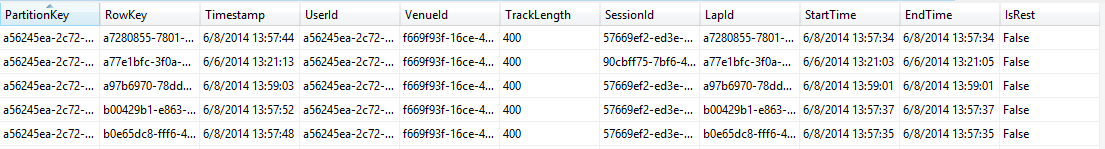
\includegraphics[width=.6\textwidth]{style/images/aggregationLapsStructure}    
  \end{center}
  \caption{De ronde leaderboard tabel, een voorbeeld van een leaderboard tabel. Hierbij is de Partition Key het account Id en de Row Key het context Id (groep, baan of account Id).}
  \label{fig:entiteiten}
\end{figure}

De structuur van de leaderboard tabellen ziet er als volgt uit.
{\color{red} tabel toevoegen}
\section{Businesslaag}
  De businesslaag bestaat uit meerdere grote onderdelen. Zowel aggregatie als de workflows zijn twee gescheiden onderdelen die zich in de businesslaag bevinden.
 
\begin{figure}[ht]
  \begin{center}
  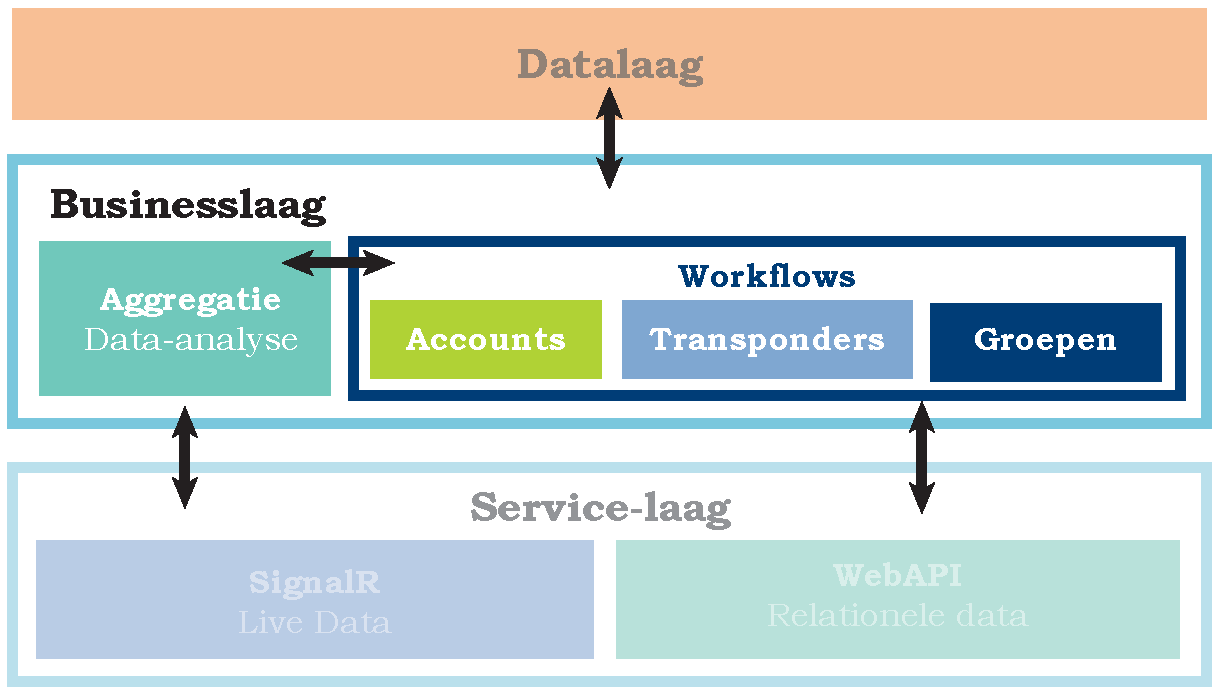
\includegraphics[width=.6\textwidth]{style/images/Businesslaag}    
  \end{center}
  \caption{Opbouw en interactie van de businesslaag}  
  \label{fig:lagen-businesslaag}
\end{figure}
  
  
  De businesslaag is de plek waar de communicatie met de datalaag en de servicelaag plaats vindt. Vanwege de keuze om de data realtime door te geven aan de applicatie is het belangrijk dat deze laag snel en vloeiend werkt, ook bij een hoge load. Om deze reden hebben we gekozen voor een Cloud-oplossing in Windows Azure, welke draait op een of meerdere Cloud instances. Bij een hogere load worden er automatisch voldoende extra instances aangemaakt en wordt de load evenwichtig verdeeld. Tevens biedt een Cloud-oplossing de mogelijkheid om verbeteringen aan bestaande of juist nieuwe functionaliteit toe te voegen aan de back-end, zonder dat de applicatie hierbij een update vereist.

Hoewel er meerdere soortgelijke Cloud-oplossingen bestaan, ging vanwege de bestaande infrastructuur van Emando de voorkeur uit naar Windows Azure. Een bijkomend voordeel van Windows Azure is de eenvoudige integratie met Visual Studio, waardoor het deployen naar de cloud- of testomgeving gemakkelijk is.

\subsection{Aggregatiestructuur}

Omdat de ruwe doorkomsten niet direct betekenis hebben voor gebruikers, dient deze data verrijkt te worden om zo inzicht te geven in trainingen van gebruikers. Dit proces noemen we de aggregatie van data.

Zodra er een doorkomst binnenkomt binnen de datalaag, wordt het Id hiervan naar de aggregatielaag overgestuurd via de Azure Service Bus. Zodra de aggregatielaag deze ontvangt, wordt de bijbehorende doorkomst opgevraagd. Hierna start het aggregatieproces, dat bestaat uit de volgende onderdelen, zoals ook te zien is in figuur~\ref{fig:aggregatie-flow}:

\begin{itemize}
\item \textbf{Reguliere filters.}
Deze filters vergelijken reeds bestaande geaggregeerde en ruwe data met de nieuwste binnenkomst, om zo nieuwe data te aggregeren. Deze data wordt vervolgens doorgegeven aan de dispatchers en top filters. Voorbeeld: Het opmaken van rondetijden aan de hand van verschillende doorkomsten op een baan.
\item \textbf{Top filters.}
Deze filters vergelijken reeds bestaande geaggregeerde data met de zojuist geaggregeerde data, om zo te kijken of de zojuist geaggregeerde data een record bevat voor de gebruiker. Deze filters verwerken de nieuwe records in de leaderboards voor een gebruiker op gebruikers-, baan- en groepsniveau. Vervolgens worden deze leaderboards doorgegeven aan de dispatchers. Voorbeeld: Een gebruiker heeft een nieuwe ronde geschaatst, waarin zijn rondetijd verbeterd is, maar ook zijn totale afstand op de baan toegenomen is. 
\item \textbf{Dispatchers.}
De dispatchers ontvangen alle geaggregeerde data en zijn verantwoordelijk voor het doorgeven van deze data aan de juiste applicaties. De dispatchers zorgen er voor dat deze data realtime binnen komt bij alle geïnteresseerden van deze updates. 
Voorbeeld: Live doorkomsten van gebruikers van een groep/baan. 
\end{itemize}

De filters zijn opgebouwd volgens een pipeline-structuur. Na het uitvoeren van een filter worden de filters aangeroepen die de filteruitvoer als invoer verwachten. Als een filter geen aggregatie uit kan voeren, stopt de aggregatie bij dit filter, aangezien er zonder de uitvoer van dit filter, geen andere filters aangeroepen kunnen worden. 

\begin{figure}[h]
  \begin{center}
    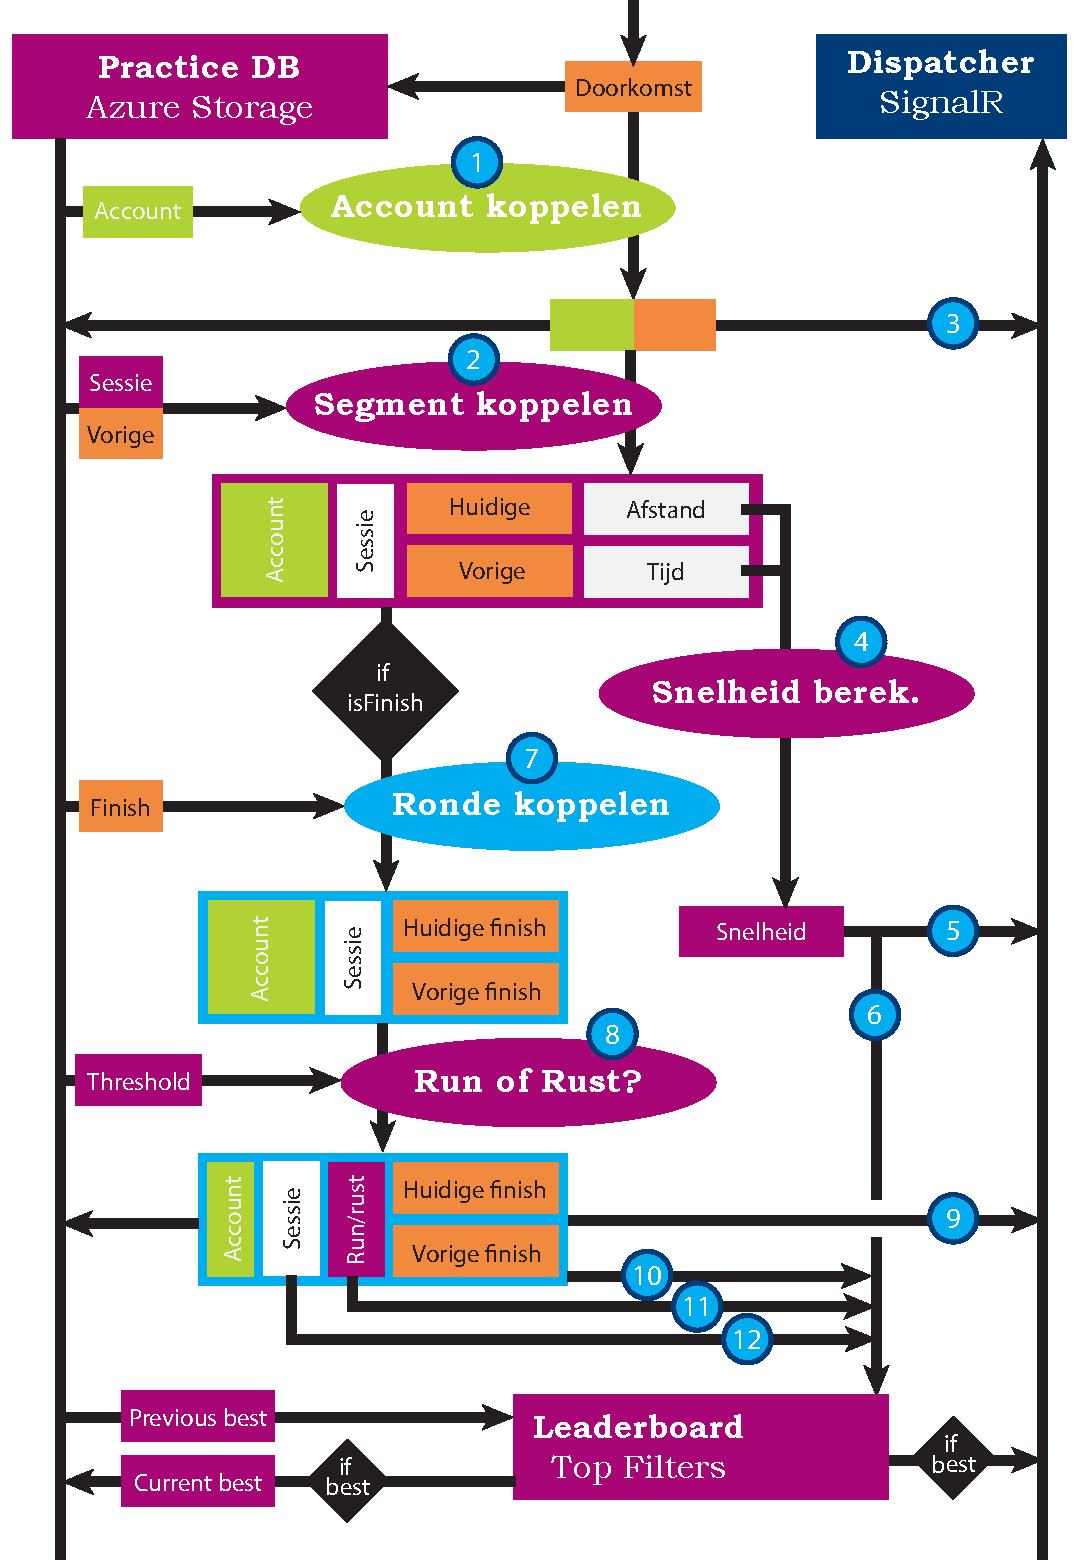
\includegraphics[width=.4\textwidth]{style/images/Aggregatie-flow}
  \end{center}
  \caption{Flow-diagram van het aggregatieproces \\ N.B. Deze afbeelding is in groot formaat opgenomen in Appendix~\ref{ch:aggregation-flow} op pagina~\pageref{fig:aggregatie-flow-large}.}
  \label{fig:aggregatie-flow}
\end{figure}

\begin{enumerate}

\item \textbf{Account koppelen aan doorkomsten.}

Allereerst wordt bij een doorkomst aan de hand van het transponder nummer een account gezocht. Als er een bestaande gebruiker is die dit transpondernummer momenteel aan zijn account gekoppeld heeft, wordt dit account gekoppeld aan deze doorkomst. Dit wordt opgeslagen in een aparte tabel in Azure Table Storage.

\item \textbf{Doorkomsten koppelen aan segmenten.}
Een doorkomst maakt deel uit van een training, soms gekoppeld aan een trainingsschema. Een training kan bestaan uit een of meerdere sessies. Een segment van doorkomsten houdt in dat er twee doorkomsten van dezelfde gebruiker binnen 30 minuten hebben plaatsgevonden op dezelfde baan. Wanneer de vorige doorkomst van deze gebruiker en de huidige doorkomst binnen een segment vallen, vallen deze doorkomsten onder dezelfde trainingssessie. Wanneer dit het geval is, krijgt de doorkomst dezelfde sessie Id toegewezen als zijn vorige doorkomst. Wanneer dit niet het geval is of wanneer er geen vorige doorkomst is, kan er geen segment gevonden worden.

\item \textbf{Dispatchen van live doorkomsten.}
Zodra er een gebruiker gevonden is bij een doorkomst, moet deze doorgegeven worden aan alle ``geïnteresseerden'': de gebruiker zelf, gebruikers op dezelfde baan, leden van dezelfde groep als deze gebruiker en alle gebruikers die geabonneerd zijn op deze gebruiker.

Met behulp van SignalR wordt de doorkomst doorgegeven aan de juiste personen.

\item \textbf{Snelheid berekenen.}
Tussen twee doorkomsten in een segment ligt een bepaalde afstand. Een gebruiker heeft deze afstand afgelegd in een tijdsinterval. Aan de hand van deze gegevens wordt de snelheid binnen dit segment berekend.

\item \textbf{Dispatchen van snelheden.}
Zodra er een snelheid is berekend voor een gebruiker op een bepaald segment, moet deze doorgegeven worden aan alle eerder genoemde geïnteresseerden.

Met behulp van SignalR wordt de doorkomst doorgegeven aan de juiste personen.

\item \textbf{Snelheidsleaderboard updaten en dispatchen.}
Zodra er een snelheid berekend is over een bepaald segment, kan dit gevolgen hebben voor het snelheidsleaderboard. De gereden snelheid wordt vergeleken met de eerdere persoonlijke records van de gebruiker, zijn records op deze baan en zijn records in al zijn groepen. Daarnaast wordt altijd de gereden afstand op de baan, tijdsinterval etc. bijgewerkt in de totalen binnen dit leaderboard. Wanneer de zojuist gereden snelheid een record blijkt te zijn voor een van zojuist genoemde contexten, wordt deze up to date gebracht in de leaderboards. Daarna wordt het gehele leaderboard voor deze context via SignalR naar alle geïnteresseerden verstuurd.

\item \textbf{Doorkomsten koppelen aan rondes.}
De gevonden sessie bij het segment kan gebruikt worden om rondes te vinden. Wanneer de huidige doorkomst afkomstig is van de finish-lus en de gebruiker in de huidige sessie een eerdere doorkomst op de finish-lus heeft, is er sprake van een ronde in een training. 
Wanneer de sessie Ids niet overeenkomen, of de huidige doorkomst niet op de finish lijn ligt is het niet mogelijk om een ronde te vinden.

\item \textbf{Filteren van run- en rustperiodes.}
Afhankelijk van het type sporter, wordt er al dan niet getraind aan de hand van een trainingsschema. Deze schema's bestaan vaak uit run- en rustperiodes waarin respectievelijk hard getraind wordt of langzaam wordt uitgereden. Omdat de lengte van rondes kan variëren op verschillende banen, wordt niet aan de hand van tijden, maar snelheden gefilterd. Wanneer de gemiddelde snelheid in een ronde hoger is dan een vooraf ingestelde snelheid, wordt deze ronde beschouwd als een run-ronde. Anders wordt deze beschouwd als onderdeel van een rustperiode. Nu alle ronde data compleet is, wordt deze ronde opgeslagen in een aparte tabel in Azure Table Storage voor latere aggregaties.

\item \textbf{Dispatchen van rondes.}
Zodra er een ronde is berekend voor een gebruiker, wordt deze opnieuw met behulp van SignalR naar de eerder genoemde geïnteresseerden verstuurd.

\item \textbf{Rondeleaderboard updaten en dispatchen.}
Zodra er een ronde is gevonden voor een gebruiker, kan dit gevolgen hebben voor het rondeleaderboard. De gereden ronde wordt vergeleken met de persoonlijke records voor een gebruiker, zijn records op deze baan en zijn records in al zijn groepen. Daarnaast wordt altijd de gereden afstand op de baan, tijdsinterval etc. bijgewerkt in de totalen binnen dit leaderboard. Wanneer de zojuist gereden rondetijd een record blijkt te zijn voor een van zojuist genoemde contexten, wordt deze up to date gebracht in de leaderboards. Daarna wordt het gehele leaderboard voor deze context naar alle geïnteresseerden gestuurd via SignalR.

\item \textbf{Run/rustleaderboard updaten en dispatchen.}
Zodra er een ronde is gevonden voor een gebruiker, kan dit gevolgen hebben voor het run/rustleaderboard. De gereden rondetijd wordt toegevoegd aan de desbetreffende run/rustperiode en aan de hand hiervan wordt het totaal hiervan vergeleken met de persoonlijke records voor een gebruiker, zijn records op deze baan en zijn records in al zijn groepen. Daarnaast wordt altijd de gereden afstand op de baan, tijdsinterval etc. bijgewerkt in de totalen binnen dit leaderboard. Wanneer de zojuist gereden rondetijd een record blijkt te zijn voor een van zojuist genoemde contexten, wordt deze up to date gebracht in de leaderboards. Daarna wordt het gehele leaderboard voor deze context naar alle geïnteresseerden gestuurd via SignalR.

\item \textbf{Sessie leaderboard updaten en dispatchen.}
Zodra er een ronde is gevonden voor een gebruiker, kan dit gevolgen hebben voor het sessie leaderboard. De gereden rondetijd wordt toegevoegd aan de desbetreffende sessie en aan de hand hiervan wordt het totaal hiervan vergeleken met de persoonlijke records voor een gebruiker, zijn records op deze baan en zijn records in al zijn groepen. Daarnaast wordt altijd de gereden afstand op de baan, tijdsinterval etc. bijgewerkt in de totalen binnen dit leaderboard. Wanneer de zojuist gereden rondetijd een record blijkt te zijn voor een van zojuist genoemde contexten, wordt deze up to date gebracht in de leaderboards. Daarna wordt het gehele leaderboard voor deze context naar alle geïnteresseerden gestuurd via SignalR.

\end{enumerate}

\subsection{Dataconsistentie en parallellisering}
Vanwege de meeschalende Cloud-oplossing, kan het voorkomen dat aggregaties van één persoon over meerdere instances berekend worden. Het is belangrijk dat deze aggregaties parallel lopen om gebruikers van realtime updates te kunnen voorzien. Dit brengt echter wel het probleem met zich mee dat sommige data afhankelijk is van andere data en dat deze data consistent moet blijven met elkaar. De eerder genoemde pipeline-architectuur zorgt er voor dat bij ieder filter bekend is welke afhankelijkheden hierop berusten. Zodra het filter klaar is met zijn aggregatie, wordt gekeken of de aggregatie bruikbaar is voor zijn afhankelijkheden en geeft zijn aggregatie aan de hand hiervan door. Deze afhankelijkheden kunnen op hun beurt over verschillende instances verdeeld worden, zonder dat er opstoppingen ontstaan.

Omdat onze aggregatielaag berust op de \mylaps SDK en een service bus, kan het in theorie voorkomen dat een eerdere doorkomst pas later bij deze laag binnenkomt dan een latere doorkomst. Ook kan het voorkomen dat het berekenen van een aggregatie van een eerdere doorkomst langer duurt dan die van een latere doorkomst, waardoor de updates hiervan door elkaar heen gaan lopen. Dit is te zien in figuur~\ref{fig:aggregatie-timing-problem}. 
In deze figuur is te zien hoe doorkomst~3 later gereden wordt, maar eerder geaggregeerd wordt dan doorkomst~2 welke eerder gereden is. Doordat de aggregatie werkt met de vorige doorkomst (doorkomst~1) wordt doorkomst~3 gekoppeld aan doorkomst~1 in een segment waarover de snelheid berekend wordt. Hieruit komt een correcte waarde.

Wanneer doorkomst~2 echter geaggregeerd wordt, vraagt deze de vorige doorkomst op. Omdat doorkomst~3 al geaggregeerd was, is doorkomst~3 zijn vorige doorkomst. Hierbij wordt doorkomst~2 gekoppeld aan doorkomst~3. In dit segment blijkt nu -100 meter gereden te zijn. Er zou nu een verkeerde aggregatie ontstaan!

Daarom is het belangrijk dat de data te allen tijde consistent is, ook over meerdere Cloud instances.
Om deze reden zijn alle repositories calls voorzien van een synchronisatietijdstip. Dit is het tijdstip waarop de doorkomst doorgekomen is. Deze calls geven daarmee alleen (aggregatie)data terug die op het moment van de doorkomst beschikbaar was. In het bovengenoemde geval zou doorkomst~2 daarom óók gekoppeld worden aan doorkomst~1, vanwege het feit dat doorkomst~3 later binnen gekomen is dan doorkomst~2. Op deze manier worden inconsistenties in de data voorkomen.

\begin{figure}[ht]
  \begin{center}
    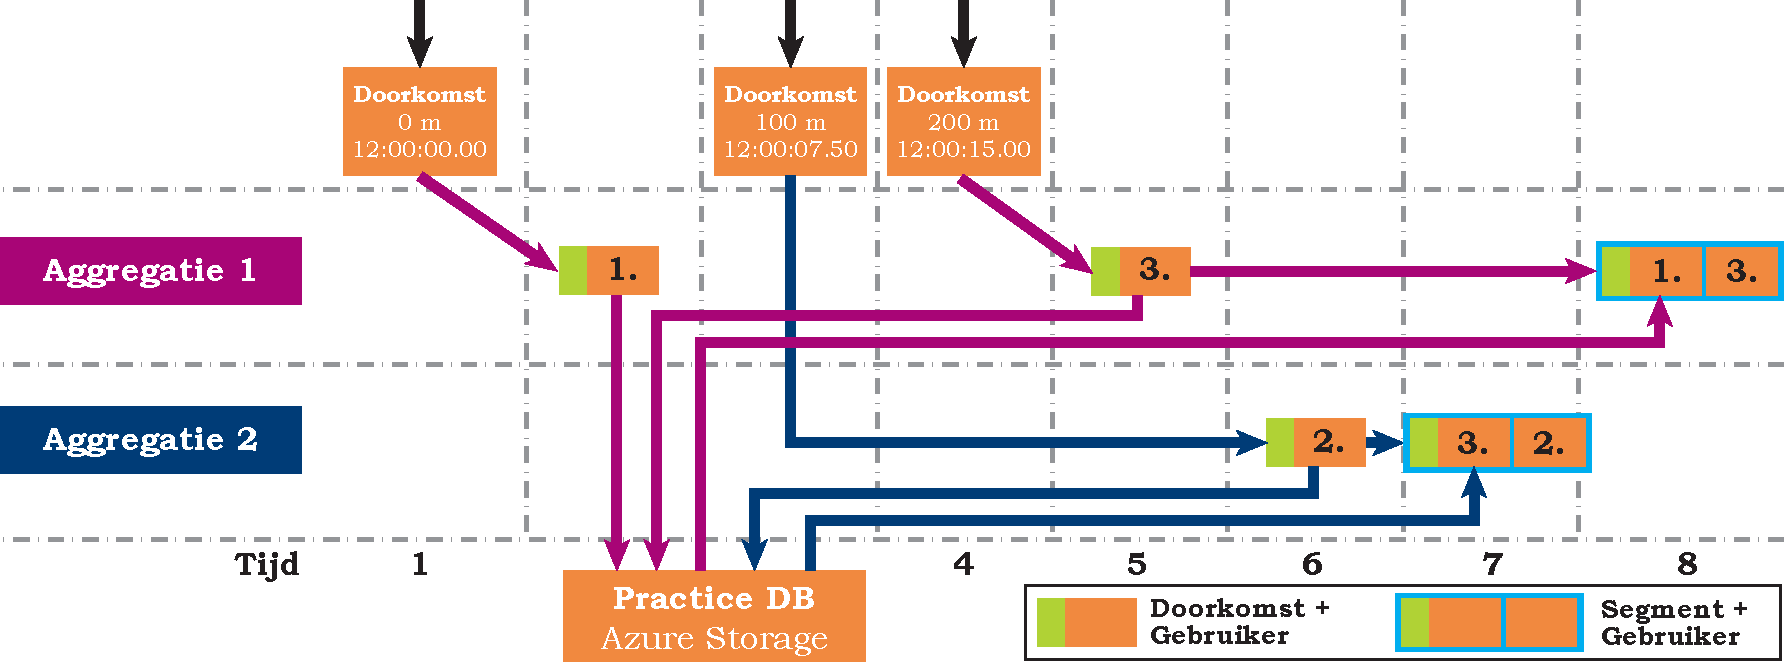
\includegraphics[width=\textwidth]{style/images/aggregatie-timing-problem}
  \end{center}
  \caption{Flow-diagram van hoe de data stroom verkeerd kan gaan.}
  \label{fig:aggregatie-timing-problem}
\end{figure}

Voor de leaderboards is gekozen om deze te verspreiden over vier aparte tabellen. Leaderboards bestaan uit data die vanuit verschillende filters aangepast worden. Hierbij wordt eerst het leaderboard opgevraagd en daarna de update teruggeschreven naar de tabel. Bij het updaten is het mogelijk om een merge-operatie uit te voeren, waarbij alleen de beschikbare data (bijvoorbeeld een snelheidsleaderboard) bij te werken zonder daarbij de bestaande data aan te passen. Dit kan echter alleen wanneer de ETag-eigenschap van dit leaderboard ondertussen niet gewijzigd is. Deze ETag-eigenschap is een onderdeel van Azure Table Storage dat bijhoudt of het record in de tussentijd al dan niet gewijzigd is. In de praktijk komen tussentijdse wijzigingen vaak voor, doordat er meerdere filters parallel aan elkaar hetzelfde record bij proberen te werken voor andere leaderboard eigenschappen. Om deze reden is beter om de leaderboards te spreiden over meerdere tabellen.


  \subsection{Workflows}

Een onderdeel van de Businesslaag zijn de workflows. Workflows zijn afgebakende taken, 
welke door de eenvoudig door de servicelaag en andere businesslaagprocessen zijn aan te roepen, 
en waarbij de servicelaag niet hoeft te weten hoe de taken worden uitgevoerd, 
als er maar het beoogde resultaat oplevert. In onze applicatie zijn er op 3 gebieden workflows, zoals ook te zien is in figuur~\ref{fig:lagen-businesslaag}:

\begin{itemize}
	\item{\textbf{Gebruikersaccounts beheren.}} 
	De AccountWorkflow biedt mogelijkheden om accounts aan te maken met zowel gebruikersnaam en wachtwoord als met een Facebook authenticatie sleutel (``access token''). Verder kunnen accounts worden opgezocht aan de hand van hun emailadres of unieke nummer. De servicelaag biedt deze workflow rechtstreeks aan via de API.

	\item{\textbf{Transponders beheren.}} 
	Gebruikers kunnen per tijdseenheid maar één transponder hebben en deze kan niet door meer mensen tegelijk geregisteerd zijn. Deze logica wordt verzorgt voor de servicelaag, zodat gebruikers transponders kunnen toevoegen en kunnen ontkoppelen van hun account en daar de juiste eventuele foutmeldingen bij krijgen. Daarnaast moet de businesslaag snel kunnen opzoeken welke gebruiker bij een transponder hoort, op het moment dat een doorkomst binnenkomt. De TransponderWorkflow bevat de logica ervoor om deze checks te doen en de transponders op te zoeken.

	\item{\textbf{Groepen beheren.}} 
	Het aanmaken en beheren van groepen zijn ook specifieke taken waar een GroupWorkflow voor bestaat. Deze workflow zorgt er voor dat de actieve gebruiker wordt toegevoegd aan de aangemaakte groep en dat er alleen wijzigingen plaatsvinden die mogen worden uitgevoerd. Deze logica voornamelijk door de servicelaag gebruikt, om de groepen functionaliteit aan te bieden. Daarnaast wordt beschikbare nieuwe informatie doorgestuurd naar de gebruikers uit dezelfde groepen. Ook hiervoor wordt de workflow gebruikt.

\end{itemize}
  
\section{Servicelaag}
  Onze applicatie bevat data met verschillende relevantie over tijd. Tijdens het sporten zijn vooral doorkomsten interessant evenals informatie over de actuele training. Ná het sporten zijn vergelijkingen met andere sporters interessant en analyses op de training. Zowel SignalR\footnote{\url{http://www.asp.net/signalr}} als WebApi\footnote{\url{http://www.asp.net/web-api}} zijn technieken om data door te sturen, maar SignalR is gemaakt voor live data en WebApi voor het toegankelijk maken van al bestaande data via een REST API~\footnote{\url{http://en.wikipedia.org/wiki/Representational_state_transfer}}. In onze applicatie gebruiken we dan ook beide technieken naast elkaar. Een derde techniek die we gebruiken is OWIN~\footnote{\url{http://www.asp.net/aspnet/overview/owin-and-katana}}, een brug tussen de webserver en de web-applicatie. OWIN verzorgt het opstarten en configureren van de web-applicatie.

\subsection{SignalR}
SignalR onderhoudt een continue verbinding tussen server en client waarbij het zelf zorgt voor het juiste onderliggende protocol. SignalR werkt bij voorkeur over WebSockets, maar werkt ook met oudere browsers door gebruik te maken van "polling". Bij polling houdt de server de verbinding zolang mogelijk open. Als er een bericht afgeleverd moet worden wordt deze verstuurd, de verbinding wordt gesloten, en er wordt weer een nieuwe verbinding gemaakt. Door gebruik te maken van SignalR hoeven we ons niet bezig te houden met de werking van deze ingewikkelde protocollen, en kunnen we eenvoudig een verbinding opzetten.

Naast het beheren van de individuele verbindingen, onderhoudt SignalR ook virtuele groepen. Een nieuw bericht kan gestuurd worden naar individuele gebruikers, maar ook naar deze groepen. Wij gebruiken de groepen als interesse-context: in onze applicatie kunnen gebruikers een scherm open hebben van een baan of een (vrienden)groep, ze zijn dan geïnteresseerd in de updates van alle gebruikers in die context. Wanneer één van de leden van de context aan het schaatsen is, en er moet een update gestuurd worden, dan sturen we met één commando aan iedereen die in die context een update.

\subsection{WebApi}
De API die we gemaakt hebben met WebApi 2.0 ontsluit data die niet ``live'' is. Onder andere de registratie en het ophalen van profieldata, groepen, favorieten en banen gebeuren via WebApi. WebApi heeft als voordeel dat het te gebruiken is zónder een SignalR client en ook dat het makkelijker te debuggen is dan SignalR, omdat er geen  websocketverbinding gemaakt hoeft te worden. Door een API aan te bieden kan ons platform in de toekomst ook gemakkelijk gebruik worden voor andere applicaties.

\subsection{OWIN}
Zowel SignalR als WebApi zijn als 'middleware' geconfigureerd in het opstartscript van OWIN. OWIN zorgt er voor dat een binnenkomend verzoek wordt afgehandeld door die middleware die het verzoek kan afhandelen. Zo worden verzoeken naar de api doorgestuurd naar WebApi en verzoeken naar de url /signalr worden doorgestuurd naar SignalR. 

In OWIN hebben we ook OAuth geconfigureerd. OAuth is een authenticatiestandaard waarbij een gebruiker kan inloggen met zijn gebruikersnaam en wachtwoord of via een externe dienst zoals Facebook. De client krijgt dan een "token", een sleutel, die meegestuurd moet worden met opvolgende verzoeken. Hiermee is de authenticatie centraal geregeld, want zowel SignalR als WebApi kunnen hier mee overweg.
  \subsection{Platform-onafhankelijke client}
Om in de mobiele applicatie de data van zowel SignalR als WebApi te ontsluiten is er een platform-onafhankelijke client gemaakt. Deze client bevat alle interactie met SignalR en WebApi zodat andere delen van de applicaties geen verbinding hoeven op te zetten en te onderhouden.

De client bevat dus methodes voor zaken als inloggen en registreren, welke zijn aangesloten op WebApi. Deze methodes zijn asynchroon en retourneren taken. Met de asynchrone taalelementen van C\#\footnote{\url{http://msdn.microsoft.com/en-us/library/hh191443.aspx}} kunnen eenvoudig de functies worden aangeroepen vanuit knoppen in de applicatie en worden taken afgewacht, zodat óf de voortgangs-indicator kan worden verborgen óf een foutmelding getoond kan worden.

De data die vanuit SignalR binnenkomt wordt als ``Observable'' weergegeven. Observables zijn taalelementen van C\# uit \ac{rx} en kunnen worden gezien als objecten die functies uitvoeren als er nieuwe data binnenkomt, door een functie te ``subscriben'' op een Observable. De data vanuit SignalR heeft het karakter van bijvoorbeeld \textit{de actuele snelheid van gebruiker X}. De Observable heet dan CurrentSpeed en een voorbeeld van een functie is er een die de snelheid op het telefoonscherm aanpast aan de net binnengekomen snelheid.

\subsection{Lokale opslag met Akavache}
Mobiele applicaties moeten anders omgaan met data dan desktop-applicaties in die zin dat mobiele applicaties elk moment gesloten kunnen worden. Telefoons hebben een beperkte hoeveelheid geheugen, en als het OS van de telefoon detecteert dat er te weinig geheugen vrij is kan een niet zichtbare applicatie abrupt worden afgesloten. Als een gebruiker onze applicatie even onderbreekt om een andere applicatie te bekijken dan kan de applicatie dus zomaar worden afgesloten. Om bij het terug komen in de applicatie na het afsluiten niet een leeg scherm te hoeven tonen, moeten we data opslaan op het permanente geheugen van de telefoon. Hiervoor gebruiken we Akavache\footnote{\url{https://github.com/akavache/Akavache}}.

Akavache is een library voor asynchrone en persitente key-value opslag voor C\# applicaties. Met Akavache is eenvoudig te checken of een model al geladen is, het eventueel nog te downloaden en dan op te vragen. 

Aangezien de ViewModels, die ook later nog aan bod komen in sectie ~\ref{sec:vm-reactive-ui}, niet opgeslagen kunnen worden (sommige eigenschappen kunnen niet worden geserialiseerd) moet er nog een vertaalslag plaatsvinden tussen de opgeslagen entiteiten en de ViewModels. Onze platform-onafhankelijke client doet dit voor alle entiteiten en zorgt er voor dat  de ViewModels in stand blijven gedurende de hele tijd dat de applicatie draait. Eventuele wijzigingen worden aangepast in de ViewModels, maar de ViewModels worden nooit vervangen.

\section{Presentatielaag}
  De presentatielaag bevind zich in de mobiele applicatie. Hieronder komen enkele karakteristieke onderdelen aan bod.
  \subsection{View Models en Reactive UI} 
\label{sec:vm-reactive-ui}

Voor de koppeling tussen views en data gebruiken we speciale ViewModels die een `lifetime' hebben die langer is dan de views die deze modellen gebruiken. Controllers vragen de ViewModels op en geven ze door aan de views. Elke view bind zich vast aan het ViewModel en als een veld van het model verandert, dan updaten de views automatisch. Dit werkt met ReactiveUI~\footnote{\url{http://www.reactiveui.net/}}, een UI framework dat gebruikmaakt van \ac{rx}. Elk veld van de ViewModels stuurt een notificatie naar alle luisterende views als het wordt aangepast. ReactiveUI levert hiervoor zowel het notificatie-systeem als het koppel systeem voor views. Een versimpeld voorbeeld is als volgt:

\begin{verbatim}
public class SpeedViewModel : ReactiveObject {
  private double _speed = 0;
  public double Speed { 
    get { return _speed; }
    set { RaiseAndSetIfChanged(ref _speed, value); }
  }
}

public class View : UIView, IViewFor<SpeedViewModel> {
  public View(SpeedViewModel model) {
    OneWayBind(
      model, vm => vm.Speed, 
      view => view.speedLabel.Text, 
      field => field.ToString("F") + " km/h"
    );
  }
}
\end{verbatim}
%\caption{Voorbeeld van ReactiveUI: een ViewModel en View}

Wanneer de controller nu een ViewModel aanpast, of er via SignalR een update binnenkomt, dan wordt de view direct aangepast. 

Naast het updaten van alleenstaande modellen, gebruiken we ook lijsten van modellen. Hiervoor gebruiken we ReactiveList's, uit ReactiveUI, welke notificaties kunnen sturen wanneer er een element wordt toegevoegd of wordt verwijderd uit de lijst. We updaten dan de bestaande tabel en hoeven niet de hele tabel opnieuw te tekenen.

Door gebruik te maken van ReactiveUI wordt het heel simpel om views te maken die `live' zijn en het zorgt er voor dat de code overzichtelijk blijft, omdat het invullen en updaten van de views met dezelfde code gebeurt en deze erg simpel is.

\subsection{Grafische user interface}

{\par \bigskip \par \color{red} TODO: Belachelijk veel screenshots toevoegen \par \bigskip \par }

De gebruikersinterface van de applicatie staat in principe los van de rest van de applicatie. Hoewel het grootste deel van de code gebruikt kan worden op verschillende platforms, moet de gebruikersinterface voor elk platform apart ontwikkeld worden. Tijdens dit bachelorproject is ervoor gelozen om alleen een specifieke gebruikersinterface te maken voor iPhones. Zoals eerder besproken, is hiervoor gekozen omdat het grootste deel van de KNSB top een iPhone gebruikt. Wanneer zij besluiten dat de applicatie ook daadwerkelijk gebruikt gaat worden, kunnen er nog gebruikersinterfaces gebouwd worden voor andere populaire platforms.

Door het gebruik van Xamarin gaat de implementatie van de iOS user interface iets anders dan met reguliere iOS applicaties. Er kan deels gebruikgemaakt worden van het Interface Builder onderdeel van Xcode, de officiele ontwikkelomgeving voor iOS. Na het opslaan van de gebruikersinterface in Xcode, genereert de Xamarin omgeving bestanden waarmee de interface kan worden aangesloten op C\#.

De gebruikersinterface van de applicatie is in twee lagen gestructureerd. Allereerst zijn er de verschillende tabs waarmee de gebruiker kan wisselen tussen de verschillende contexten: persoonlijk, favorieten, groepen en banen. Deze onderverdeling is geïmplementeerd met behulp van de in iOS ingebouwde TabViewController. Voor elk van deze contexten hebben we geprobeerd een icoontje te ontwerpen dat overeen komt met de stijl die in iOS 7 wordt gehandhaafd, maar tegelijkertijd ook duidelijk genoeg aangeeft wat er met het icoontje bedoeld wordt. Voor de gebruikers, favorieten en groepen was dit redelijk simpel, maar voor de banen was dit toch een grotere uitdaging, aangezien de baan er voor verschillende sporten anders uitziet. Daarom hebben we uiteindelijk besloten om een weg te gebruiken voor het representeren van banen.

\begin{figure}[H]
\centering

\includegraphics[width=0.6\textwidth]{style/images/TabView}
\caption{De iOS TabView}
\label{fig:tab-view}
\end{figure}

De tweede laag van de interface-structuur bestaat eigenlijk voor een groot deel uit overzicht-detail schermen. Het profielscherm van een gebruiker bevat bijvoorbeeld een overzicht van al zijn sessies, een sessiescherm is weer een overzicht van alle runs, met daarin weer de afzonderlijke rondes. Deze structuur, die ook voorkomt bij de favorieten, groepen en banen, wordt geimplementeerd met behulp van een XXXNavigationController.

Binnen ongeveer alle schermen wordt er gebruikgemaakt van tabel-views. Om deze views realtime te kunnen voorzien van actuele data, zijn er speciale tabel-viewcontrollers ontwikkeld die aansluiten op de reactive ViewModels. Telkens als er iets wordt aangepast in de ViewModels zal deze tabel-viewcontroller de nodige tabelcellen invoegen, verwijderen, verplaatsen of bijwerken.

Een ander belangrijk deel van de gebruikersinterface is de functionaliteit die ervoor zorgt dat er grafiekjes getekend worden. Dit wordt gedaan met behulp van de CoreGraphics functies in iOS. Het was hierbij belangrijk dat ook deze grafieken automatisch bijgewerkt worden als de data verandert. Dit is gedaan door […]. Helaas had dit wel tot gevolg dat de applicatie erg langzaam werd. Als oplossing hiervoor worden de grafieken waarvan het onwaarschijnlijk is dat deze zullen veranderen, omgezet in afbeeldingen en opgeslagen.

\section{Testomgeving}
Bij elke applicatie is het van belang dat er goed getest wordt. In het geval van onze applicatie was het toch een behoorlijke uitdaging om effectief te testen. Allereerst werkt de applicatie met realtime data van een externe leverancier. Deze data kan gesimuleerd worden, maar het is lastig om unit-tests te maken die realtime en asynchrone datastromen kunnen testen. Daarnaast is het testen van een iOS App vrij lastig en tijdrovend, aangezien het veel tijd kost om vingerbewegingen te simuleren, te controleren of deze de gewenste gevolgen hebben en of de juiste data getoond wordt.

Gezien het feit dat de App lastig te testen is, terwijl het grootste gedeelte van de App de data vanuit de server direct overneemt in de views, hebben we besloten de App handmatig te testen. De server daarentegen wordt wel uitgebreid getest met behulp van automatische unit-tests. 

Binnen het server-gedeelte van de applicatie worden alle transponder-doorkomsten realtime verwerkt. De filters die te maken hebben met het verwerken van deze doorkomsten worden elk afzonderlijk getest om er zeker van te zijn dat ze correct functioneren. Dit testen wordt gedaan met een set unit-tests die elk van deze filters aanroept met bepaalde input en controleert of de uitvoer overeenkomt met de verwachte uitvoer van deze filters.

{\par \bigskip \par \color{red} TODO: Screenshots van testomgeving toevoegen \par \bigskip \par }

Dit houdt in dat in elke test een nep-omgeving wordt gecreëerd. Deze omgeving bevat de gebruikers, groepen en relaties die tijdens de test voor het betreffende filter gebruikt worden. Alle hulpklassen voor het filter worden gemockt, wat inhoudt dat er een gesimuleerd object wordt gemaakt dat het gedrag van de oorspronkelijke klasse nabootst. Tijdens de tests wordt gecontroleerd of de juiste methoden van de hulpklassen worden aangeroepen en of de juiste uitvoer wordt geproduceerd.

Al deze tests worden uitgevoerd in de testomgeving van Visual Studio. In deze omgeving kan men zien welke tests slagen of falen en kan in debug-modus achterhaald worden wat de oorzaak is van falende tests.

\subsection{Integratietesten van client en server}
Een bijkomend voordeel van het hebben van een platformonafhankelijke client is dat een deel van de App ook uit te voeren is op hetzelfde platform als waar de server draait. Dit heeft tot gevolg dat er toch integratietests uitgevoerd kunnen worden om te controleren of de App aansluit op de server. Ook maakt dit het debuggen makkelijker, aangezien je  in Visual Studio door de programma's heen kan `steppen' (het regel voor regel door de lopende applicatie heen stappen).

In Figuur~\ref{fig:integratie-project} zijn de schermen te zien die onderdeel uitmaken van het integratietestproject. Het scherm bij \subref{fig:integratie-azure} is de Azure Emulator, hierin worden de datalaag, businesslaag (de Aggregatie) en servicelaag (de API) uitgevoerd. Bij \subref{fig:integratie-passing-input} kunnen er met behulp van het toetsenbord transponderdoorkomsten worden gesimuleerd, die vervolgens in Azure worden verwerkt. Ten slotte wordt in \subref{fig:integratie-client} getoond welke data de API Client binnen krijgt.

\begin{figure}[ht]
\centering
\subfigure[De Azure Emulator]{
    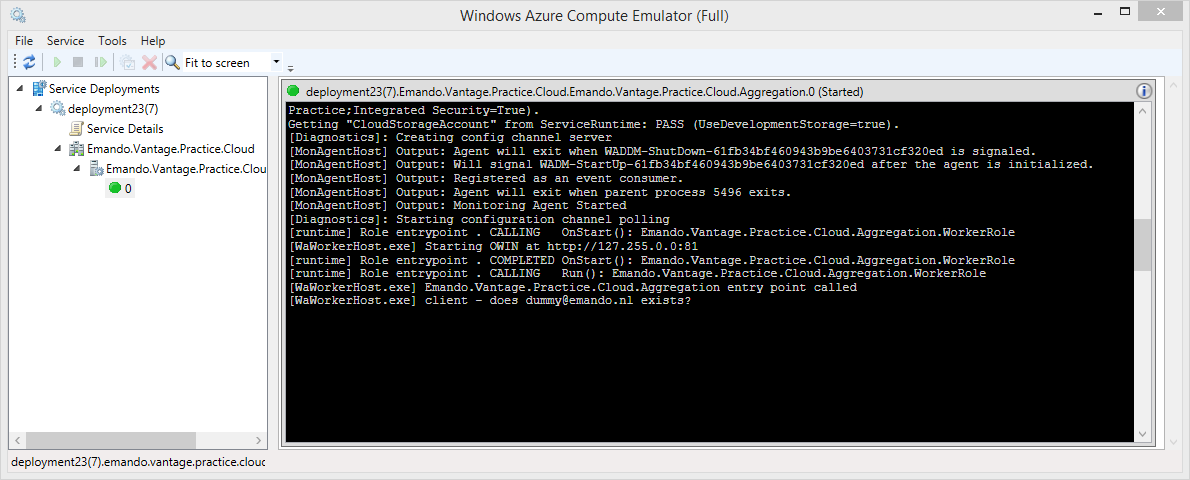
\includegraphics[height=5cm]{style/images/screenshots/IntegrationAzure}
    \label{fig:integratie-azure}
}

\subfigure[De Passing Input Console]{
    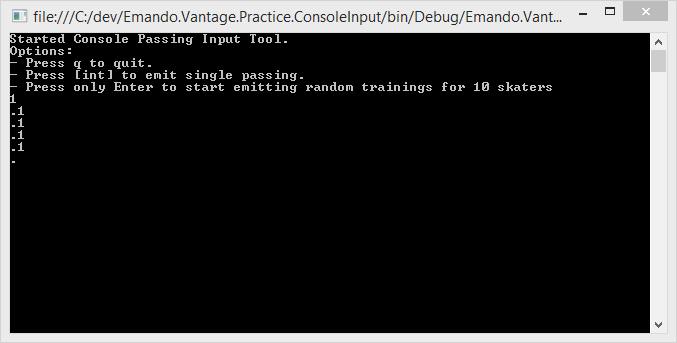
\includegraphics[height=4cm]{style/images/screenshots/IntegrationPassingInput}
    \label{fig:integratie-passing-input}
}

\subfigure[De Client Console]{
    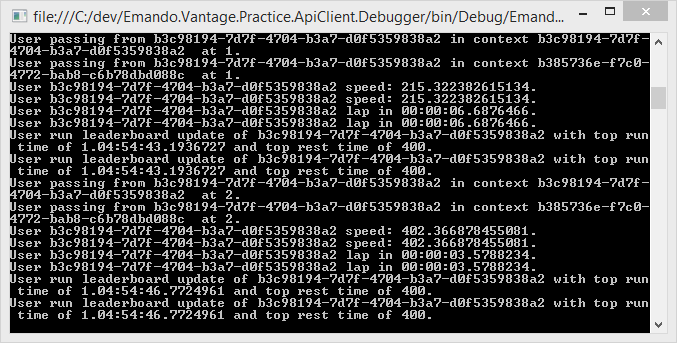
\includegraphics[height=4cm]{style/images/screenshots/IntegrationClient}
    \label{fig:integratie-client}
}
\caption{Het integratieproject voor het testen van de API Client}
\label{fig:integratie-project}
\end{figure}

Het is niet mogelijk een test van het hele platform te automatiseren op zo'n manier dat alles op een test-server draait. Voor het uitvoeren van het Azure project is een Azure Service Bus nodig die alleen in de Cloud bestaat. Azure is alleen te bereiken met de Azure SDK die alleen voor Visual Studio beschikbaar is, en dus alleen op Windows werkt, terwijl de Xamarin projecten voor iOS alleen op een MacBook kunnen opstarten. Om een speciale Mac test-server op te zetten met daarop een virtuele machine met Windows was te veel werk voor dit project, dus worden integratie-tests uitgevoerd op onze persoonlijke MacBooks, waar we deze set-up wel hebben geïnstalleerd.

% TODO: we moeten nog integratie tests schrijven in iOS.Test

\chapter{Evaluatie} \label{ch:evaluatie} \section{Gebruikers testen}

\section{\acs{sig} feedback}
De \acf{sig} heeft onze broncode tweemaal geëvalueerd.

\chapter{Discussie} \label{ch:discussie} Voorafgaand aan het project zijn zowel op proces- als product-niveau een aantal beslissingen genomen. Deze beslissingen hebben een directe invloed gehad op het resultaat en de werkwijze van het project. In dit hoofdstuk worden een aantal van deze keuzes geëvalueerd aan de hand van de bevindingen en resultaten gedurende het project. 

\section{Product}

\subsection{Hoe af is de applicatie?}
Bij de oplevering van het project staat er een werkende applicatie die sporters op een gemakkelijke en overzichtelijke manier inzicht geeft in hun trainingen, maar ook in die van anderen. Daarnaast bevat de applicatie een sociale component die sporters kan motiveren om tot het uiterste te gaan. Deze sociale component zorgt er voor dat sporters de applicatie willen blijven gebruiken. De applicatie berust op een robuuste en uitbreidbare API welke goed gedocumenteerd is. Het is daarmee relatief eenvoudig om extra functionaliteit toe te voegen.

\subsection{Verbeteringen}
Hoewel de applicatie voldoet aan de door ons gedefiniëerde MVP, zijn er enkele verbeterpunten welke toevoegingen kunnen zijn aan de applicatie. Zo zou het mogelijk kunnen zijn om realtime training informatie door te geven aan sporters met behulp van audio cues. 
Verder zou de geaggregeerde data gecombineerd kunnen worden met trainingstijden om gebruikersprofielen te creëren, welke gebruikt kunnen worden om gebruikers suggesties aan te kunnen bieden om met andere sporters van gelijkwaardig niveau te gaan sporten.
Ook is het mogelijk om het sociale component verder uit te breiden naar een achievement systeem. 

Tot slot zou ook het delen van prestaties en records en het exporteren van deze data naar RunKeeper een toevoeging zijn voor de applicatie.

\subsection{Android}
Momenteel is de applicatie slechts beschikbaar voor één mobiel platform: iOS. Naast iOS is ook Android een groot platform waar veel gebruikers van onze doelgroep mee werken, hetgeen de \ac{KNSB} reeds aan heeft gegeven in een van de meetings met Emando. Om het bereik van de applicatie te vergroten, is het aan te raden om de applicatie ook uit te rollen voor Android. Vanwege de cross-platform ontwikkeling met Xamarin, is het slechts nodig om de platform specifieke views te schrijven voor dit platform. Om deze reden kan dit in relatief weinig tijd.

\subsection{Is de applicatie een toevoeging op de reeds bestaande markt?}
Hoewel er zeker ruimte is voor toevoegingen van en verbeteringen aan de huidige applicatie, bevat de applicatie tal van functionaliteiten welke trainingen voor sporters op een overzichtelijke manier inzichtelijker kunnen maken. Naast het inzien van eigen data, is het ook mogelijk om andermans data in te zien, hetgeen een toevoeging is voor trainingsgroepen en coaches. 
Hoewel deze twee aspecten an sich niet nieuw zijn, is de eenvoud en combinatie er van in één applicatie dat wel. Verder is het sociale component niet terug te vinden in vergelijkbare reeds beschikbare applicaties.

Uit de enquêtes en gebruikerstest is gebleken dat de applicatie veel potentie heeft en er zeker vraag naar is op onder sporters. Hieruit kwam naar voren dat er veel vraag is naar extra functionaliteit (met name de audio-cues), maar de ondervraagden gaven hierbij aan de applicatie met de huidige functionaliteit ook al graag in gebruik te nemen.

\section{Proces}

\subsection{SCRUM overhead}
Omdat de precieze vormgeving van de applicatie naast het MVP niet vast stond en er veel Cutting Edge technieken gebruikt werden met nieuwe mogelijkheden, bleek de flexibele ontwikkelmethode SCRUM een goede oplossing voor ons project. Hiermee was het gedurende het project mogelijk om de doelstellingen en implementatiedetails per sprint bij te stellen. Ondanks het feit dat iedere sprint opnieuw gepland moest worden en dagelijkse standups nodig waren om de projectvoortgang en planning door te spreken, heeft SCRUM veel flexibiliteit en overzicht geboden binnen het project. Het gebuik van SCRUM raden wij dan ook ten zeerste aan bij een volgend (soortgelijk) project.

\subsubsection{Effectiviteit \ac{tfs}}
Bij de planning van het project en het werken in sprints hebben we veelvuldig gebruik gemaakt van \ac{tfs}. Hoewel dit een handige tool is, welke binnen Emando de standaard was bij het plannen van sprints, zit er bij het plannen veel overhead. Omdat iedere functionaliteit opgesplitst moest worden in verantwoordelijkheden, backlog items met verantwoordelijkheden en corresponderende taken met een tijdsbesteding, zat er veel tijd in het op orde houden van de planning en voortgang binnen \ac{tfs}. Ondanks het feit dat Visual Studio goede integratie met \ac{tfs} biedt, dienen taken ook handmatig op orde gehouden te worden om bij de dagelijkse standups een goed beeld van de voortgang van het project te verkrijgen.

Omdat onze opdrachtgever een controlerende rol heeft aangenomen binnen het project, bood \ac{tfs} een uitkomst om op ieder moment gemakkelijk inzicht te verkrijgen in de projectvoortgang en afhankelijkheden. Ook tijdens het project was het voor ons erg prettig om in \ac{tfs} altijd een overzicht te hebben van alle taken en prioriteiten. 

Ondanks het feit dat het inplannen van sprints in \ac{tfs} relatief veel tijd heeft gekost, heeft dit ons in combinatie met de dagelijkse standups veel tijd bespaard doordat het een helder overzicht van de projectvoortgang en afhankelijkheden. Het gebruik van \ac{tfs} sprint planning tools als \ac{tfs} raden wij dan ook ten zeerste aan bij een volgend project.

\subsection{Burndown \& afhankelijkheden}
In \ac{tfs} is het mogelijk om aan de hand van de gemaakte sprint planning een burndown grafiek te genereren, waarin in te zien is hoe de projectvoortgang in een sprint verloopt. Bij het plannen van de sprint dienen daarbij een exact aantal uur per taak aangegeven te worden. Door het gebruik van veel Cutting-Edge technieken die nieuw waren voor ons, hebben sommige taken veel meer en andere veel minder tijd gekost dan aanvankelijk gedacht. Vanwege de onderlinge afhankelijkheden was het soms lastig om verder te gaan met taken die berustten op andere taken die vertraging op liepen. Omdat deze taken op \ac{tfs} bij een vertraging niet afgevinkt konden worden, bevat de burndown grafiek daarom veel pieken en dalen en week het merendeel van de dagen de burndown grafiek af van de ideale werklijn. 

Ook bleek bij gedurende sprint regelmatig dat er voor bepaalde taken op de achtergrond extra taken nodig waren om deze naar behoren te laten functioneren. Bij het aanmaken van nieuwe taken binnen \ac{tfs} met corresponderende uren ontstond dan ook een stijgende lijn in de burndown grafiek, omdat er extra uren aan het project toe waren toegekend.


\subsection{Verwachtingen verschillende betrokkenen}
Bij het project waren aanvankelijk 3 partijen betrokken: De opdrachtgever, de TU Delft begeleider en de project leden.
Later is door het contact tussen Emando en KNSB ook de KNSB betrokken bij het project. 

Omdat de verwachtingen van alle betrokkenen van elkaar afweken, is gezien de tijdsdruk er gekozen voor een middenweg waarin iedereen zich kon vinden. Daarbij is gekozen voor een applicatie die gemakkelijk uitbreidbaar is en voldoet aan alle eisen van MVP (en waar mogelijk meer), voorzien is van een robuuste en stabiele back-end en een goede documentatie van het project en zijn voortgang.  

\subsubsection{Contact met opdrachtgever}
Om goed contact te onderhouden met de opdrachtgever is er voor gekozen om 4 dagen per week op het kantoor van Emando te werken in Amsterdam. Dit maakte het mogelijk om de verwachtingen, project-voortgang en -planning regelmatig af te stemmen in de dagelijkse standups. Ook zorgde dit er voor dat implementatie details en Code Reviews gemakkelijk doorgesproken konden worden, zodat alle implementaties volgens de bedrijfsstructuur van Emando gerealiseerd konden worden.

\subsection{Cutting-edge technieken}
Bij het maken van implementatie keuzes is regelmatig bewust gekozen voor cutting-edge technieken. Hoewel het gebruik van de nieuwste technologieën veel mogelijkheden met zich meebrengt, kost het gebruiken van deze technieken meestal meer tijd dan het gebruiken van conventionele technieken. Bij het maken van deze afweging was het niet alleen de technische uitdaging, maar met het oog op het toekomstperspectief van de applicatie bleek het verstandig om nieuwe technologieën met veel potentie te gebruiken. Deze technologieën zullen in de toekomst (hoogstwaarschijnlijk) langer ondersteund blijven dan conventionele technieken.
Hierbij zijn alleen technologieën gebruikt die reeds ondersteund werden door de desbetreffende community.

Ondanks het feit dat deze technologieën een steilere learning-curve hebben dan conventionele technieken, boden deze technieken dusdanig meer mogelijkheden dat dit opwoog tegen de benodigde extra tijd.

\chapter{Conclusie} \label{ch:conclusie} De applicatie is in het kader van het Bachelor Eindproject ``Trainingsapp voor baansporten'' ontwikkeld. Omdat de projectduur van dit project vele malen korter is dan het traject van een volledige applicatie, is de applicatie niet compleet. Zoals beschreven is in de resultaten van de gebruikerstest en de discussie in hoofdstuk~\ref{ch:discussie}, zijn er tal van functionaliteiten waarmee de applicatie later uitgebreid kan worden. Het is daarom belangrijk dat het project goed opgeleverd wordt, zodat de applicatie door ontwikkeld kan worden.

\section{Oplevering}
Alle code die ontwikkeld is binnen het project is terug te vinden binnen Source Control van het project in \ac{tfs}.
Om eventuele doorontwikkeling van het project te bevorderen bevatten is alle code, waar nodig, voorzien van commentaar. Ook zijn er voor de API's documenten gemaakt waarin hun werk- en gebruikswijze gedocumenteerd is. 

Naast deze documentatie voor de code, is er ook een aantal documenten geschreven waarin beschreven staat hoe andere ontwikkelaars aan de slag zouden kunnen met het project. Hierin staat de volgorde van stappen beschreven die ondernomen dient te worden om alle afhankelijkheden en cloud instances draaiende te krijgen.

\section{Doorontwikkeling}
Hoewel de applicatie momenteel geschikt is om uit te brengen op de markt, zijn er nog tal van mogelijkheden om de applicatie door te ontwikkelen. Zoals uit de enquêtes en de meetings met de \ac{KNSB} gebleken is, is er veel vraag naar de applicatie, maar ook naar verdere functionaliteit. 
Enkele van deze gewenste functionaliteiten zijn:

\begin{itemize}
\item Profielen/groepen/trainingsdata onvindbaar maken voor anderen (handig voor topsporters).
\item Audio cues, live audio feedback over je training 
\item Integratie met hartslagmeter
\item Schatting voor calorieën verbruik
\item Integratie met instelbare trainingsschema's en suggesties hiervoor aan de hand van training resultaten
\item Mogelijkheid om te trainen met GPS, i.p.v. transponders
\end{itemize}

Ook een vergroting van de doelgroep door de applicatie uit te brengen op andere platformen is wenselijk. Binnen \ac{tfs} zijn backlog items aangemaakt voor alle functionaliteit die later wenselijk is, maar nog niet geïmplementeerd is. Deze backlog items zijn gesorteerd op volgorde van prioriteit en kunnen gebruikt worden als leidraad bij de doorontwikkeling van het project.

In het theoretische geval dat er een Azure Cloud instance crasht kan het voorkomen dat er aggregaties meerdere malen berekent. Dit resulteert niet in ``verkeerde'' data, maar kan wel zorgen voor dubbele berekeningen over intervallen. Dit probleem is te verhelpen door aggregaties niet te laten werken met een synchronisatietijdstip, maar in plaats daarvan aggregaties die vertraagd raken, de ``te vroeg'' uitgerekende aggregaties te laten verwijderen en opnieuw uit te laten rekenen. In overleg met Emando is er voor gekozen dit probleem niet op te lossen tijdens dit Bachelorproject omdat de kans dat een dergelijke Cloud instance crasht bijzonder klein is en het oplossen van dit probleem op technisch vlak een grote hoeveelheid tijd zou kosten. Dit is een probleem dat in de doorontwikkeling zeker verholpen kan worden.

\section{Toekomst}
De \ac{KNSB} heeft in overleg met Emando besloten de mogelijkheden van huidige applicatie mee te nemen in de nieuwe strategie voor het seizoen 2014-2015 om actieve sporters te benaderen. De \ac{KNSB} denkt momenteel na over een complete applicatie die naast het trainingsgedeelte ook andere schaatsgerelateerde functionaliteiten zou bevatten. Deze functionaliteiten zouden onder andere informatie over verenigingen, informatie over (veilig) natuurijs, openingstijden en adressen van schaatsbanen etc. kunnen omvatten. Het is nog onduidelijk of de huidige applicatie uitgebreid zal worden met functionaliteit en platformen of dat er een complete schaats-applicatie komt waar de gebouwde functionaliteit onderdeel van zal uitmaken. 

Het is in ieder geval zeker dat de \ac{KNSB} veel potentie ziet in de gebouwde functionaliteit en deze functionaliteit ook graag wil aanbieden aan de Nederlandse schaatsers.

%% Use letters for the chapter numbers of the appendices.
\appendix

\addtocontents{toc}{\protect\setcounter{tocdepth}{1}}

% Appendices, zoals
% - Definities en afko's
% - Ontwerpen/schetsen
% - UML diagrammen van architectuur
% - Gebruikerstest verslagen
% - SIG resultaten
% - API documentatie?
% - Bibliografie

\chapter{Plan van Aanpak} \label{ch:plan-van-aanpak} \section{Introductie}

\ifx\aanleiding\undefined
\newcommand{\aanleiding}{}

\begin{wrapfigure}{r}{4cm}
  \begin{center}
    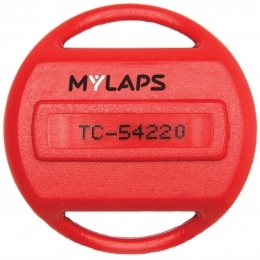
\includegraphics[width=4cm]{style/images/transponder}
  \end{center}
  \caption{MyLaps ProFlex transponder, op schaal}
  \label{fig:transponder}
  \vspace{15mm}
\end{wrapfigure}

In baansporten is de laatste jaren een ontwikkeling gaande om tijdregistratie te digitaliseren door het gebruik van transponders (bijvoorbeeld de MyLaps ProFlex transponder in Figuur~\ref{fig:transponder}) en detectie-lussen (Figuur~\ref{fig:detection-loop}) in de baan. Door deze ontwikkeling zijn nieuwe mogelijkheden ontstaan om ook naast het wedstrijdmoment de sportprestaties in te zien. Het constateren van de hierna genoemde nieuwe mogelijkheden was de aanleiding van dit project.

\begin{wrapfigure}{r}{4cm}
  \begin{center}
    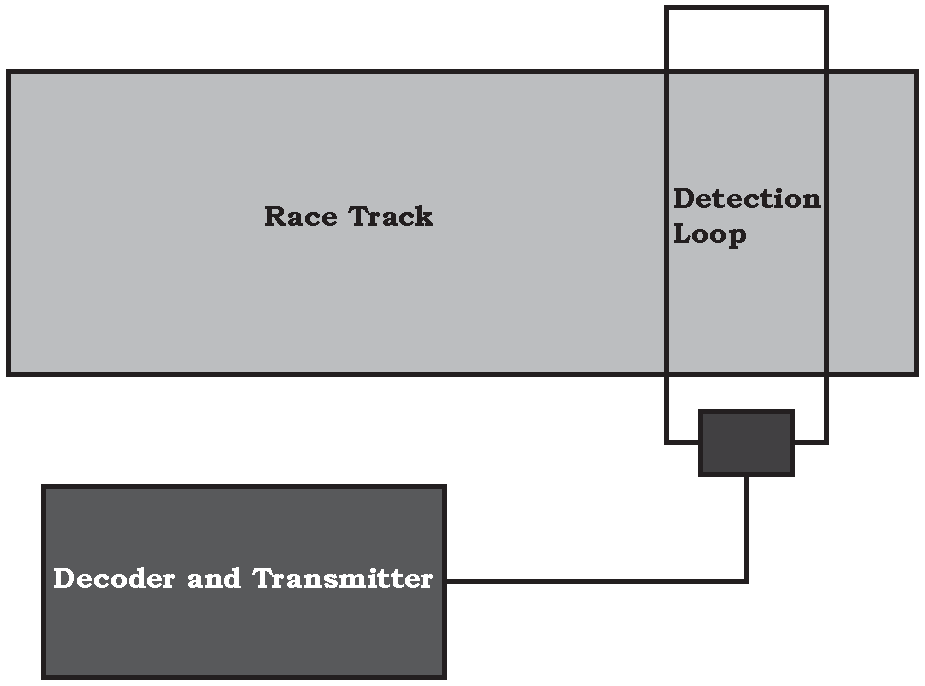
\includegraphics[width=4cm]{style/images/DetectionLoop}
  \end{center}
  \caption{Een schema van een detectielus en en decoder}
  \label{fig:detection-loop}
  \vspace{5mm}
\end{wrapfigure}

Een grote speler op de tijdregistratie-markt is MyLaps\footnote{\url{http://www.mylaps.com}}. Dit bedrijf installeert en beheert detectie-lussen en is actief bij diverse sporten zoals schaatsen, wielrennen, zwemmen, atletiek en diverse motorsporten. Bij sporten met permanente banen liggen de detectie-lussen het gehele jaar in de baan. Er bestaat de mogelijkheid om op de website van MyLaps doorkomst-tijden in te zien. De informatie die uit deze tijden is af te leiden, wordt door sporters als erg waardevol gezien om zich willen blijven verbeteren, waardoor er steeds meer getraind wordt met deze transponders.

\begin{figure}
  \begin{center}
    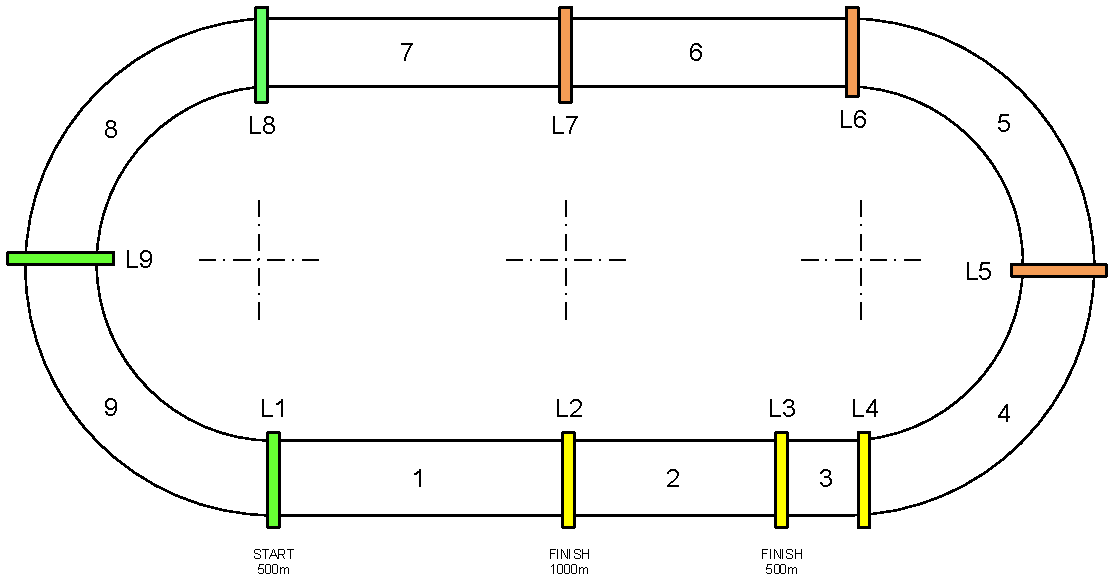
\includegraphics[width=0.8\textwidth]{style/images/BaanoverzichtHaarlem}
  \end{center}
  \caption{L1 tot en met L9 zijn de negen MyLaps transponderlussen in Haarlem}
  \label{fig:track-transponders}
\end{figure}

Voor aanvang van het seizoen worden door MyLaps detectielussen geïnstalleerd. De lussen bevinden zich in het ijs of onder het houten oppervlak van een baanwielrenbaan. Elke lus heeft een elektromagnetisch veld. Wanneer een sporter met transponder over dat veld heen rijdt, wordt de transponder geactiveerd en stuurt deze een unieke puls, die de lus opvangt. De MyLaps X2 server die aan de lussen zit aangesloten stuurt vervolgens het signaal door naar de MyLaps Cloud.

Het huidige gebruik van transponders - buiten wedstrijden - is voornamelijk achteraf, terwijl juist tijdens de training zowel sporter als coach het meeste bezig zijn met de prestaties. Het is daarom wenselijk om de resultaten in real-time door te geven aan coaches en sporters zelf.

Op veel banen zijn meerdere detectie-lussen geïnstalleerd, terwijl er op de website van MyLaps slechts één wordt ontsloten. In Thialf, de schaatsbaan in Heerenveen, Friesland, liggen bijvoorbeeld twaalf detectie-lussen, in Haarlem (Figuur~\ref{fig:track-transponders}) negen en op de andere schaatsbanen liggen er tenminste twee. Door de data van meerdere lussen te combineren is een betere indicatie te maken van de snelheid van sporters.

\begin{wrapfigure}{r}{0.4\textwidth}
 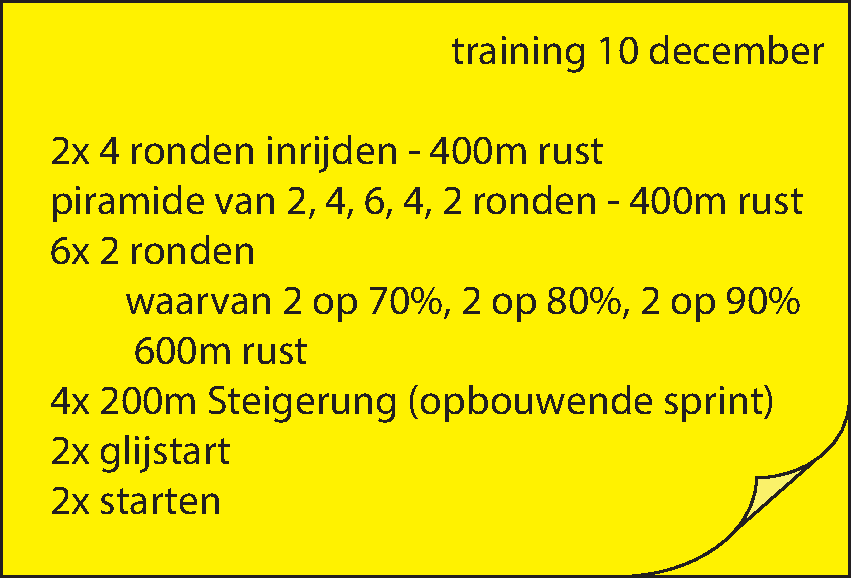
\includegraphics[width=0.4\textwidth]{style/images/training}
 \caption{Een typisch schaats-trainingsschema}
\end{wrapfigure}

Trainingen, bij bijvoorbeeld schaatsen, bestaan uit losse trainingsonderdelen. Allround schaatsers moeten bijvoorbeeld 4 ronden warmrijden, dan 6 keer 2 ronden sprinten, dan 4 keer een sprintje van 200 meter, 2 keer een glijstart en dan 2 keer een echte start bij de coach, vanuit de zijkant van de baan. Tussendoor is er rust, zo is het gebruikelijk om na een opdracht tenminste 400 meter uit te glijden. Het verschil tussen training en rust is af te leiden uit de verhouding tot de maximale snelheid.

Veel trainingselementen bestaan dus uit korte opdrachten, waar het juist om snelheid gaat. Een enkele lus is dan niet afdoende, omdat de rust voor of na de opdracht mee wordt gewogen. Sporters starten en stoppen namelijk niet precies boven de lus, maar starten vaak na de bocht en stoppen afhankelijk van de afstand van de opdracht op een willekeurig punt. 

Andere trainingen van bijvoorbeeld lange afstands- of marathonschaatsers kunnen bestaan uit één element: de hele training lang schaatsen, zonder overeind te komen. Wanneer er op tactische punten detectie-lussen geïnstalleerd zijn, is er bijvoorbeeld ook onderscheid te maken tussen bochten en de rechte stukken. Bij sporten met een ronde baan verschilt de snelheid in de bocht namelijk erg met die op het rechte eind. Deze vergelijking gebeurt nu al in Thialf, in het professionele circuit tijdens wedstrijden op televisie.

Topsporters zijn enorm prestatiegericht en als je al aan de top zit, dan kunnen kleine aanpassingen aan je techniek, ademhaling et cetera, grote verschillen maken. Coaches van professionele teams houden zich daarom bezig met allerhande analyses. Naast ademanalyse en hartslag monitoring, is het in Thialf bijvoorbeeld ook mogelijk om (van maximaal 20 schaatsers) continu de positie te bepalen met een in-door positioning system (IPS) ontwikkeld door InnoSportLab\footnote{\url{http://www.innosportlabthialf.nl}}.

Al deze geavanceerde analyses zijn echter te duur en kosten te veel tijd voor recreatieve sporters. MyLaps X2 biedt in combinatie met ons eindproduct recreatieve sporters toch een manier om analyses uit te voeren en zich naar een hoger niveau te tillen.
\fi

Aan de hand van de projectopdracht, te lezen in Sectie~\ref{sec:projectopdracht}, en gesprekken met Johan en Cor-Paul hebben we dit Plan van Aanpak opgesteld. Dit Plan van Aanpak zal worden gebruikt als houvast bij het uitvoeren van het project en wordt daarom ook goedgekeurd door alle betrokken partijen.

In dit document zal eerst de projectopdracht aan bod komen en zal worden toegelicht hoe deze tot stand is gekomen. Vervolgens wordt toegelicht op welke wijze we te werk zullen gaan en wat onze tijdsplanning is. Hierna wordt iets dieper ingegaan op de procesmatige inrichting van het project. Tot slot zal er nog aandacht worden besteed aan kwaliteitsborging.

\section{Projectopdracht}
\label{sec:projectopdracht}
\subsection{Opdrachtomgeving}

Emando is een bedrijf dat zich momenteel onder andere richt op het ontwikkelen van Vantage. Een onderdeel van Vantage is een systeem voor tijdregistratie tijdens wedstrijden in baansporten. Een groot deel van de door Vantage gebruikte infrastructuur zou ook gebruikt kunnen worden voor de recreatieve- of amateurvariant van de sport. Hiervoor zou het project ``Trainingsapp voor Baansporten'' verschillende mogelijkheden moeten bieden.

\subsection{Doelstelling project}
Het project is bedoeld als pilot. Dit houdt in dat het een mogelijke toevoeging zou kunnen zijn aan het bestaande Vantage platform, dat momenteel vooral gericht is op wedstrijden. Emando kan met dit project ook een dienst aanbieden voor recreatieve sporters en voor trainingen om hun prestaties in te zien en te vergelijken.

\subsection{Opdrachtformulering}
In overleg met Emando is de projectopdract als volgt gedefinieerd:

\begin{quotation}
\itshape
Het ontwerpen en ontwikkelen van een systeem voor het weergeven en analyseren van (live) recreatieve en trainingsdata in de context van baansporten (bijvoorbeeld schaatsen en baanwielrennen). Dit systeem zal realtime gegevens van de baan, maar ook opgeslagen gegevens uit het verleden, inzichtelijk maken voor sporters, coaches en eventuele toeschouwers (volgers). Daarnaast zal er de mogelijkheid zijn om een sociale component en een competitie element toe te voegen, en een mogelijkheid om aggregatie op data uit te voeren.

Het systeem ondersteunt het sporten: sporters hoeven hun training niet te onderbreken, doordat audio-cue's en sport-specifieke schermen geïmplementeerd worden. De sociale component bestaat uit het volgen van vrienden (mede-sporters) en het delen van resultaten. Het competitie element zal een virtuele competitie tussen vrienden omvatten.

Technisch gezien zal er een scheiding gemaakt worden tussen de diverse toepassingen (clients) en de API. De API biedt toegang tot realtime data en de diverse modulaire (sport-specifieke) aggregaties, waarbij de mogelijkheid bestaat voor bijvoorbeeld coaches om te abonneren op meerdere sporters. De API zal gekoppeld worden op bestaande systemen die data van transponders ontsluiten.
\end{quotation}

\subsection{Op te leveren producten en diensten}
Het project zal uiteindelijk resulteren in een applicatie waarmee (live) recreatieve- en trainingsdata van baansporten wordt geanalyseerd en getoond aan sporters, coaches of toeschouwers. Verder zullen gedurende het project de volgende documenten worden opgeleverd: \begin{itemize}
\item Plan van Aanpak
\item Oriëntatie-verslag (onderdeel van verslag)
\item Programma van eisen (onderdeel van verslag)
\item Eindverslag
\item Reflectie aangaande de gang van het proces
\end{itemize}

\subsection{Specifieke producteisen}

\ifx\programmavaneisen\undefined
\newcommand{\programmavaneisen}{}
\label{sec:programma-van-eisen}

Traditioneel gezien wordt bij software ontwikkeling het MoSCoW model gebruikt. Het MoSCoW model onderscheid functionaliteiten op basis van prioriteiten. De verschillende niveau's zijn must-, should-, could- en won't-haves. De vertaling van deze niveau's spreekt voor zich.

Wij gebruiken het in combinatie met SCRUM veel gebruikte \acf{mvp} model. Hierbij wordt gedefinieerd wat het product minimaal moet kunnen om bruikbaar te zijn. In die zin komt onze \ac{mvp} dus overeen met de must-haves uit het MoSCoW model. Eventuele tegenslagen mogen er niet toe lijden dat het \ac{mvp} niet gemaakt wordt, daarom is de planning om het \ac{mvp} al in de 4e week af te hebben. Gebruikers kunnen op dat moment met de applicatie spelen en de kern-functionaliteit beoordelen.

Het \ac{mvp} biedt op zich zelf nog niet alle features die zowel wij als de opdrachtgever graag geïmplementeerd zouden willen zien. Het eindproduct zal over enkele bijzondere functies moeten beschikken, de zogenaamde `killer-features' om het product populair te maken. Deze features zijn in die zin dus vergelijkbaar met de should-haves uit het MoSCoW model.

Na het \ac{mvp} en de features die het verschil maken zijn er ook nog een aantal features die niet noodzakelijk zijn en geen groot verschil zouden maken. Deze features zijn te vergelijken met could-haves uit het MoSCoW model. We zullen zeker niet alle could-haves implementeren, en wellicht komen enkele should-features ook niet aan bod. Wellicht volgt uit een user study dat de door ons bedachte could-haves door users erg gewenste features zijn. In overleg met onze begeleiders kunnen we besluiten deze features te implementeren. Bovendien bieden de could-haves een goede leidraad bij toekomstige ontwikkeling na afloop van ons project.

\subsubsection{Must-haves (\ac{mvp})}

\begin{itemize} \parskip0pt \parsep0pt
    \item Bruikbaar als applicatie op smartphone(s)
    \item Architectuur is sport-agnostisch
    \item De sport-specifieke weergave van tijden is voor schaatsbanen geïmplementeerd
    \item Mogelijkheid om een account aan te maken
    \item Real-time transponder doorkomsten tonen van geselecteerde sporters
    \item Historische doorkomsten van een persoon, gegroepeerd per dag of training
    \item De voor bovenstaande features ontwikkelde API, moet het mogelijk maken om de API uit te breiden en de applicatie aan te passen.
\end{itemize}

\subsubsection{Should-haves}

\begin{itemize} \parskip0pt \parsep0pt
    \item Mogelijkheid om account te koppelen aan Facebook
    \begin{itemize}
        \item Mogelijkheid om prestaties en records te delen op Facebook
    \end{itemize}
    \item Audio-cues geven aan sporter over doorkomsten van een geselecteerde transponder
    \item Leaderboards tonen met sporters gerangschikt naar prestaties en disciplines (virtuele competitie), zoals:
    \begin{itemize}
        \item rondetijd (actuele/gemiddelde/snelste)
        \item snelheid (gemiddelde/snelste)
        \item cumulatieve afstand (per seizoen/week/training)
        \item rust/intensief-ratio (hoeveelheid rondjes, ratio)
        \item achievements-punten (verbeter jezelf 10\%, voor 7 uur op de baan, 2 trainingen per week)
    \end{itemize}
    
    \item Groepen-functionaliteit \begin{itemize}
        \item Mogelijkheid om een lege groep te maken
        \item Mogelijkheid om sporters uit te nodigen voor een groep
        \item Mogelijkheid om op uitnodiging in een groep te gaan
        \item Mogelijkheid om uit een groep te gaan
    \end{itemize}

    \item Zowel leaderboards als real-time doorkomst-schermen kunnen worden gefilterd op groep of baan
     
    \item Privacy instellingen bieden aan gebruikers
    \begin{itemize}
        \item Mogelijkheid om een account publiekelijk of anoniem te laten indexeren
        \item Mogelijkheid om eigen data te delen met anderen
    \end{itemize}

\end{itemize}

\subsubsection{Could-haves}

\begin{itemize} \parskip0pt \parsep0pt
    \item Suggesties krijgen om met soortgelijke schaatsers te gaan schaatsen
    \item Training kunnen exporteren naar RunKeeper\footnote{Fitness logboek platform, \url{http://www.runkeeper.com}}
\end{itemize}

\subsubsection{Won't-haves}

Het door Emando ontwikkelde systeem Vantage zal de huidige systemen voor wedstrijduitslagen vervangen. Koppelingen op het huidige systeem zouden dus snel niet meer werken en het nieuwe systeem is niet af tijdens ons project.
\begin{itemize} \parskip0pt \parsep0pt
    \item Wedstrijdloting en uitslagen bekijken
    \item Persoonlijke records tonen
\end{itemize}
\else
De specifieke producteisen zijn eerder behandeld in Sectie~\ref{sec:programma-van-eisen}.
\fi

\section{Specifieke proceseisen}
Gedurende het project zal er per teamlid 40 uur per week gewerkt worden aan het project, zoals overeen gekomen in de stageovereenkomst.
De projectwerkzaamheden zullen voor het grootste deel plaatsvinden op het kantoor van Emando te Amsterdam. 
De opdrachtgever zal ervoor zorgen dat de teamleden een werkplek hebben wanneer zij hun werkzaamheden uitvoeren op het kantoor van Emando. Om goed contact met de begeleider aan de TU Delft te behouden, zal er tevens gewerkt worden op de Technische Universiteit Delft.

Het ontwikkelproces zal \textit{agile} zijn. Dat wil zeggen dat de applicatie zal worden opgeleverd in verschillende iteraties, waarin telkens functionaliteit aan de applicatie wordt toegevoegd.
Er zal gewerkt worden met de \acl{mvp}-aanpak. Er wordt in eerste instantie een applicatie opgeleverd met precies de kern-functionaliteiten en niet meer. In een latere stadium kan er op een iteratieve wijze extra functionaliteit worden toegevoegd.

De teamleden zullen zorg uitdragen om de projectwerkzaamheden naar beste weten en kunnen uit te voeren. Daarbij worden echter geen garanties gedaan over de verwachte resultaten, zoals deze omschreven zijn in de projectopdracht.

\section{Tijdsplanning}
Iedere week zal er gefocust worden op bepaalde aspecten van het proces en functionaliteiten van de applicatie. De planning is opgenomen als Appendix~\ref{ch:planning}.

\section{Projectinrichting}

\subsection{Proces}
Naast de aspecten uit de tijdsplanning zullen we elke werkdag beginnen met een stand-up: elk teamlid vertelt gedurende maximaal tien minuten wat hij afgelopen dag bereikt heeft en wat hij van plan is die dag te doen. De opdrachtgever heeft aangegeven hier zo vaak als voor hem mogelijk is bij aanwezig te zijn. Aan het eind van elke week is er een demo. Door elke dag de problemen en uitdagingen te bespreken kunnen vertragingen zo vroeg mogelijk gedetecteerd of voorkomen worden. 

De voortgang van het proces zal worden bijgehouden door middel van een issue tracker en een (digitaal) SCRUM\footnote{\url{http://en.wikipedia.org/wiki/Scrum_(software_development)}} bord. De teamleden zullen met behulp van deze tools de voortgang van het proces inzichtelijk maken en een overzicht kunnen geven van het project.

Zoals per stagecontract afgesproken, zal er per teamlid 40 uur per week gewerkt worden aan het project, waarbij teamleden zorg zullen uitdragen om de projectwerkzaamheden naar beste weten en kunnen uit te voeren. Er is in die zin een gedeelde verantwoordelijkheid, waar teamleden elkaar zonodig bijsturing geven. 

\subsection{Resources}
De opdrachtgever stelt gedurende het project een werkplek ter beschikking in het kantoor aan het Leidseplein in Amsterdam. We zullen gedurende het project op onze eigen laptops werken. Via AcademicDownload\footnote{\url{http://academicdownload.com}} verschaft de TU Delft studenten licenties voor Windows 8.1 Enterprise. Overige licenties voor ontwikkeltools zullen door de opdrachtgever worden verzorgd.

Via \mylaps zal de opdrachtgever ons toegang verschaffen tot de transponder-data. Overige data van onder andere de KNSB zal ook via het netwerk van de opdrachtgever worden verkregen.

\section{Kwaliteitsborging}
De kwaliteit van de code kan gewaarborgd worden door het aanhouden van best practices en conventies die worden gebruikt binnen Emando. Daarnaast kan gebruik gemaakt worden van de Code Review functionaliteit die in de ontwikkeltool beschikbaar is. Hiermee kunnen teamleden elkaars code beoordelen en waar nodig verbeteren. Ten slotte zal de code voor analyse worden opgestuurd naar de \ac{sig}. Afhankelijk van de \ac{sig} resultaten, kan de code verbeterd worden waar nodig.

De kwaliteit van de opgeleverde applicatie zal worden gewaarborgd door veelvuldig te testen. Dit zal niet alleen gedaan worden door middel van unit-tests, maar ook door tijdens het proces enkele integratie-tests en user-tests uit te voeren. De resultaten uit de user-tests kunnen eventueel ook gebruikt worden om het ontwerp van de applicatie beter af te stemmen op de gebruikers.

De kwaliteit en effici\"entie van het proces zal hoog worden gehouden door het gebruik van een online projectbeheeromgeving. De opdrachtgever kan via het SCRUM bord op deze omgeving de voortgang in de gaten houden en zal bij de dagelijkse stand-ups op de hoogte worden gesteld van de voortgang van het project en eventuele problemen of uitdagingen. Deze dagelijkse stand-ups zorgen er ook voor dat misverstanden tussen de opdrachtgever en het team worden voorkomen of in een vroeg stadium kunnen worden opgelost.

\chapter{Planning} \label{ch:planning} \begin{tabular}{r l}

\hspace*{4cm} % hack
{\makeatletter
\titlestyle\color{tudelft-cyan}\Large Week 1
\makeatother}
& Opstellen plan van aanpak \\

{\makeatletter
\titlestyle\color{tudelft-cyan} 21 april - 25 april
\makeatother} & Literatuurstudie \\

{\makeatletter
\titlestyle\color{tudelft-cyan} Research
\makeatother} \\
 
\medskip \\

{\makeatletter
\titlestyle\color{tudelft-cyan}\Large Week 2
\makeatother} & Literatuurstudie \\

{\makeatletter
\titlestyle\color{tudelft-cyan} 28 april - 2 mei
\makeatother} & Verwerken resultaten literatuurstudie \\

{\makeatletter
\titlestyle\color{tudelft-cyan} Research
\makeatother} & Begin opzet architectuur \\

& Regelen benodigdheden user-test \\

\medskip \\

{\makeatletter
\titlestyle\color{tudelft-cyan}\Large Week 3
\makeatother} & Verwerken resultaten literatuurstudie \\

{\makeatletter
\titlestyle\color{tudelft-cyan} 5 mei - 9 mei
\makeatother} & Opzet architectuur data analyse server \\

{\makeatletter
\titlestyle\color{tudelft-cyan} Development
\makeatother} & Opzet architectuur API \\

& Opzet architectuur client \\
& Verwerken opzet architectuur \\
 
\medskip \\

{\makeatletter
\titlestyle\color{tudelft-cyan}\Large Week 4
\makeatother} & Ontwikkeling data analyse server \\

{\makeatletter
\titlestyle\color{tudelft-cyan} 12 mei - 16 mei
\makeatother} & Ontwikkeling API \\

{\makeatletter
\titlestyle\color{tudelft-cyan} Development
\makeatother} & Ontwikkeling client  \\

 & Voorbereiden user-test \\
 & Verwerken opzet architectuur \\
 & Verwerken ontwikkelingsproces \\
 & Verwerken opzet user-test \\
 & \textbf{Deadline:} Minimum Viable Product \\
 
\medskip \\

\hspace*{4cm} % hack
{\makeatletter
\titlestyle\color{tudelft-cyan}\Large Week 5
\makeatother} & Ontwikkeling data analyse server \\

{\makeatletter
\titlestyle\color{tudelft-cyan} 19 mei - 23 mei
\makeatother} & Integratie-tests \\

{\makeatletter
\titlestyle\color{tudelft-cyan} Development
\makeatother} & Eerste user-test \\

\medskip \\

\end{tabular}

%pagebreak hierzo

\begin{tabular}{r l}

{\makeatletter
\titlestyle\color{tudelft-cyan}\Large Week 6
\makeatother} & Toevoegen functionaliteit \\

{\makeatletter
\titlestyle\color{tudelft-cyan} 26 mei - 30 mei
\makeatother} & Verwerken inzichten uit user-test \\

{\makeatletter
\titlestyle\color{tudelft-cyan} Development
\makeatother} & Regelen benodigdheden demo bij eindpresentatie \\

\medskip \\

{\makeatletter
\titlestyle\color{tudelft-cyan}\Large Week 7
\makeatother} & Toevoegen functionaliteit \\

{\makeatletter
\titlestyle\color{tudelft-cyan} 2 juni - 6 juni
\makeatother} & Afronden eindverslag \\

{\makeatletter
\titlestyle\color{tudelft-cyan} Development
\makeatother} \\

\medskip \\

{\makeatletter
\titlestyle\color{tudelft-cyan}\Large Week 8
\makeatother} & Begin test-proces \\

{\makeatletter
\titlestyle\color{tudelft-cyan} 9 juni - 13 juni
\makeatother} & Tweede user-test \\

{\makeatletter
\titlestyle\color{tudelft-cyan} Development \& Testing
\makeatother} & Afronden product \\

 & Afronden eindverslag \\
 & \textbf{Deadline:} Opsturen broncode naar de SIG \\

\medskip \\

{\makeatletter
\titlestyle\color{tudelft-cyan}\Large Week 9
\makeatother} & Verwerken feedback user-test \\

{\makeatletter
\titlestyle\color{tudelft-cyan} 16 juni - 20 juni
\makeatother} & Verbeteren laatste problemen \\

{\makeatletter
\titlestyle\color{tudelft-cyan} Development \& Testing
\makeatother} & Afronden product \\

 & Afronden eindverslag \\
 & Voorbereiden presentatie \\
 & Verbeteren broncode aan de hand van feedback van de SIG \\

\medskip \\

{\makeatletter
\titlestyle\color{tudelft-cyan}\Large Week 10
\makeatother} & Presentatie \\

{\makeatletter
\titlestyle\color{tudelft-cyan} 23 juni - 27 juni
\makeatother} & Terugblik project \\

{\makeatletter
\titlestyle\color{tudelft-cyan} Testing \& Presentatie
\makeatother} & Overdracht code \& product \\

 & \textbf{Deadline:} Inleveren hardcopy eindverslag \\
 & \textbf{Deadline:} Opsturen broncode naar de SIG \\

\end{tabular}


%\chapter{Notulen van Meetings} \label{ch:notulen-van-meetings} %\subsection*{23 april 2014}
\label{sec:meeting-23-apr}

Aanwezig: \textit{Herman, Patrick, Hylke, Johan}

\begin{description}
\item[Tekenen overeenkomsten] De overeenkomsten zijn ondertekend.

\item[Plan van aanpak] 

\item[Ontwikkelproces] Johan vertelt dat de ontwikkelmethode \textit{SCRUM} gebruikt zal worden. In principe hebben we vrijheid om het project in te delen zoals dat ons handig lijkt. Hij wil globaal op de hoogte gehouden worden van de vorderingen. Johan zal zich een halve tot een dag in de week bezig houden met het project. Hij zal zich niet bezighouden met de documenten en presentaties die bij de TU Delft aangeleverd moeten worden.

Ideaal gezien zou het systeem opgedeeld worden in (onafhankelijke) componenten Johan zou graag zien dat er een verdeling wordt gemaakt van ``managers'' op deze componenten.

\item[Wekelijkse meeting plannen voor voortgang, doelen en taken] De dagelijkse standups staan in de agenda (waar we nog toegang toe krijgen). Wat Johan betreft hebben we dan geen wekelijkse meetings nodig.

\item[Ontwikkelomgeving en versiebeheer] Johan laat de Visual Studio Online omgeving en Visual Studio zien.

\item[Testen en MYLAPS X2 introductie] Johan laat de MyLaps X2 Manager zien.

\item[Architectuur] Johan vertelt hoe andere applicaties van Emando globaal zijn opgezet. Er zijn verschillende lagen die elk verantwoordelijk zijn voor een bepaald aspect van de applicatie. Deze lagen kunnen onafhankelijk van elkaar ontwikkeld en getest worden.

\begin{itemize}
  \item De presentatielaag bevat de User Interface.
  \item De servicelaag bevat bijvoorbeeld de API.
  \item De businesslaag bevat alle functionaliteit voor het verwerken van data.
  \item De datalaag bevat databases etc.
\end{itemize}

\end{description}

\chapter{Oriëntatieverslag} \label{ch:orientatieverslag} \section{Introductie}

Aan de hand van de projectopdracht, ons Plan van Aanpak en gesprekken met Johan en Cor-Paul hebben we dit Orientatieverslag opgesteld. Dit verslag zal worden gebruikt om inzicht te verkrijgen in de mogelijke technieken voor het ontwikkelen van mobiele applicaties en server back-ends, geschikt voor onze toepassing. Tevens zullen we hier onze keuzes voor bepaalde technieken motiveren.

\section{Abcdefg}
\label{sec:alphabet}


\chapter{Interface Ontwerpen} \label{ch:interface-ontwerpen} \begin{figure}[ht]
\centering
\subfigure[Beginscherm]{
    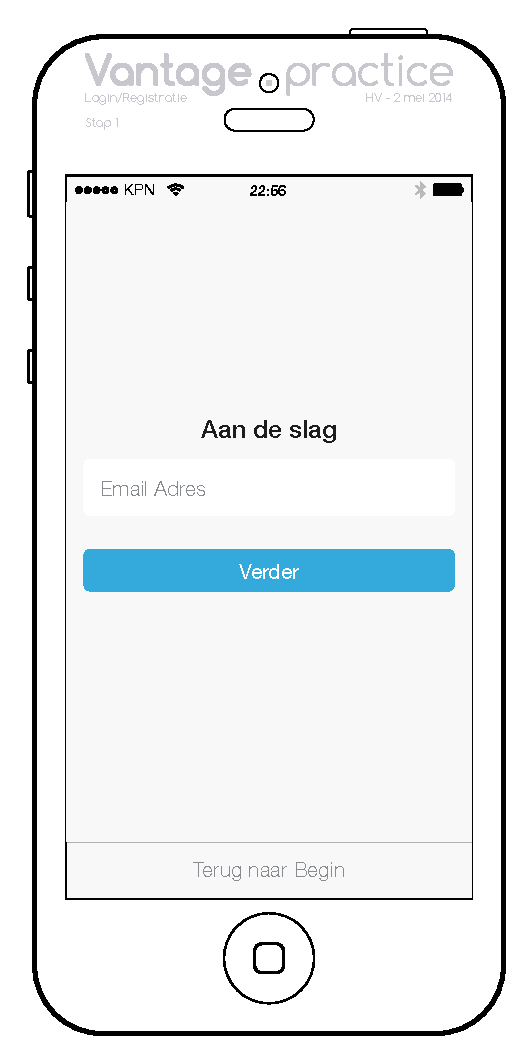
\includegraphics[width=4.5cm]{style/images/designs/02-A-Login-Registratie}
    \label{fig:login-registratie}
}
\subfigure[Registratiescherm]{
    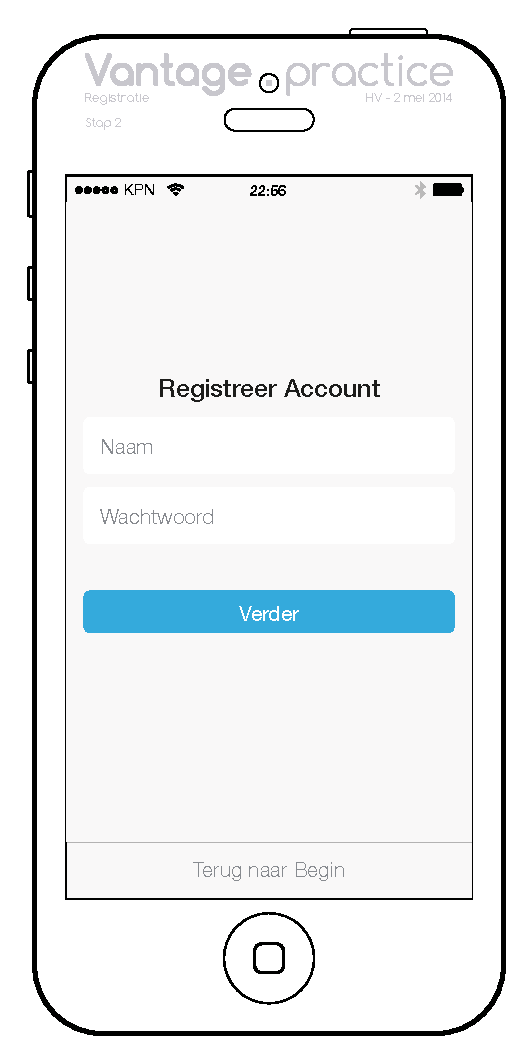
\includegraphics[width=4.5cm]{style/images/designs/02-B1-Registratie}
    \label{fig:registratie}
}
\subfigure[Loginscherm]{
    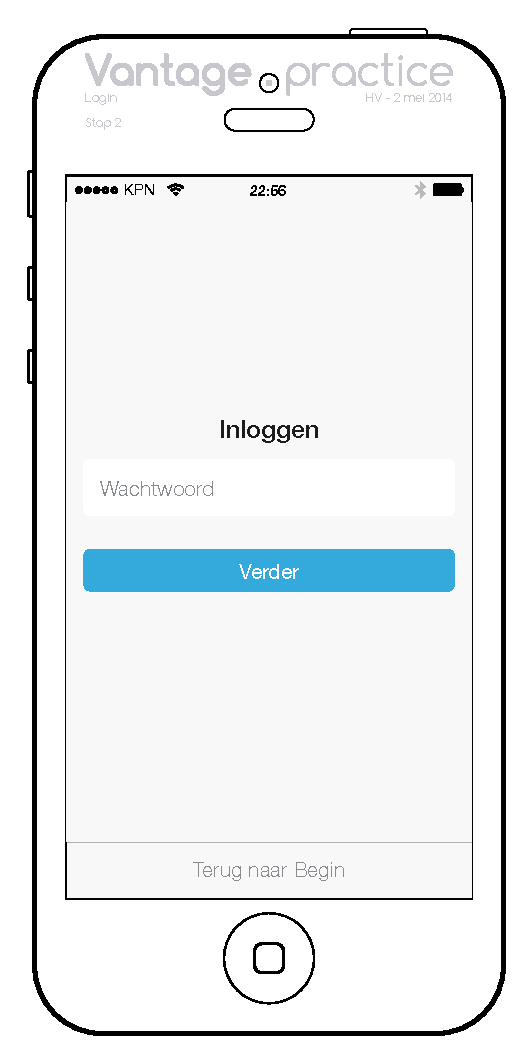
\includegraphics[width=4.5cm]{style/images/designs/02-B2-Inloggen}
    \label{fig:login}
}
\caption{Login en registratie}
\label{fig:login-en-registratie}
\end{figure}

\begin{figure}[ht]
\centering
\subfigure[Profielscherm]{
    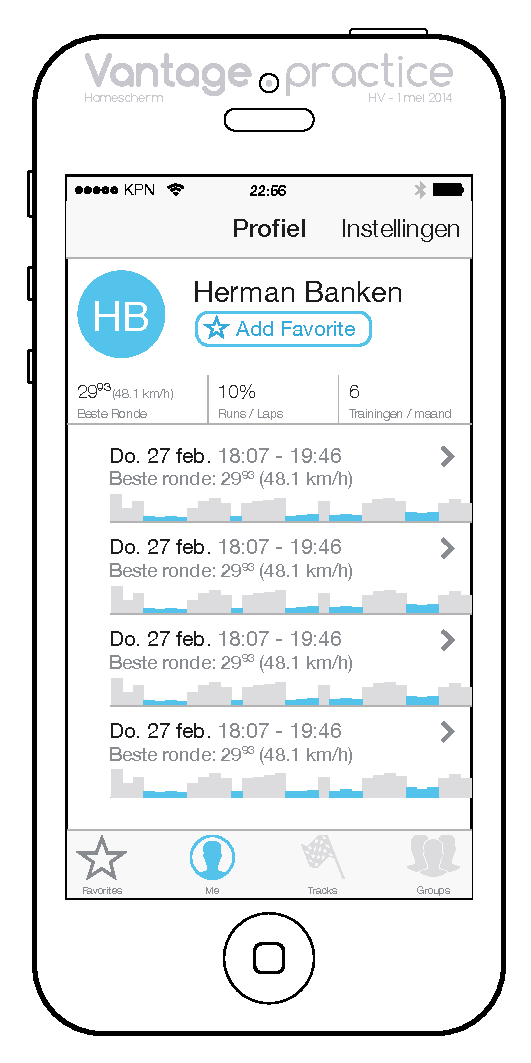
\includegraphics[width=4.5cm]{style/images/designs/03-Home}
    \label{fig:home}
}
\subfigure[Accountinstellingen]{
    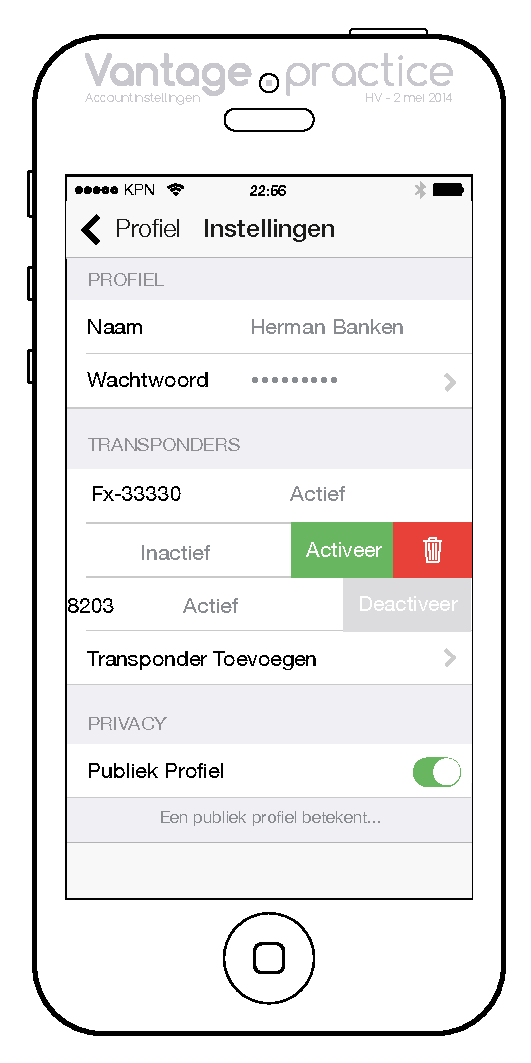
\includegraphics[width=4.5cm]{style/images/designs/04-A-Accountinstellingen}
    \label{fig:accountinstellingen}
}
\subfigure[Transponder Toevoegen]{
    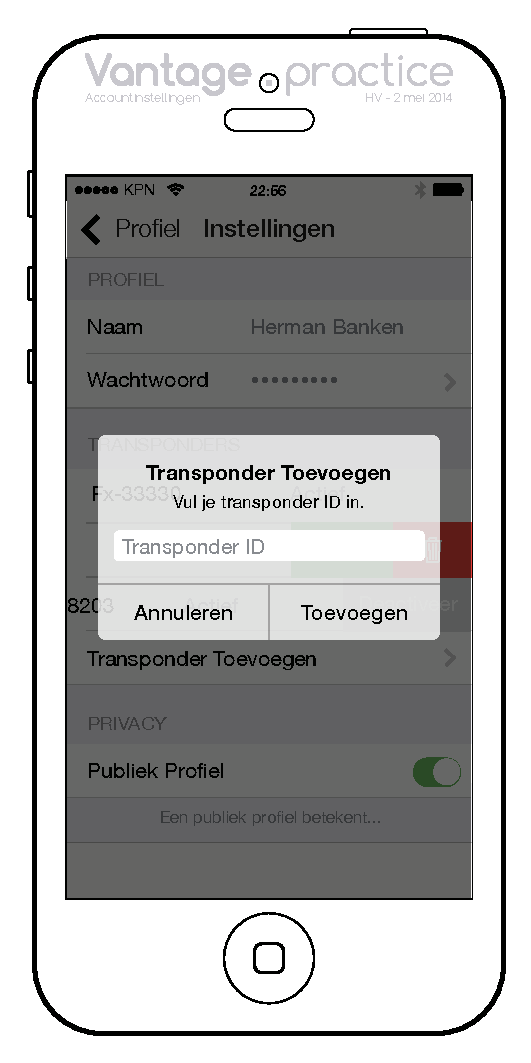
\includegraphics[width=4.5cm]{style/images/designs/04-B-Transponder_Toevoegen}
    \label{fig:transponder-toevoegen}
} % In de download ziet het er wel goed uit!
\caption{Profiel en accountinstellingen}
\label{fig:profiel-en-accountinstellingen}
\end{figure}

\begin{figure}[ht]
\centering
\subfigure[Sessieoverzicht]{
    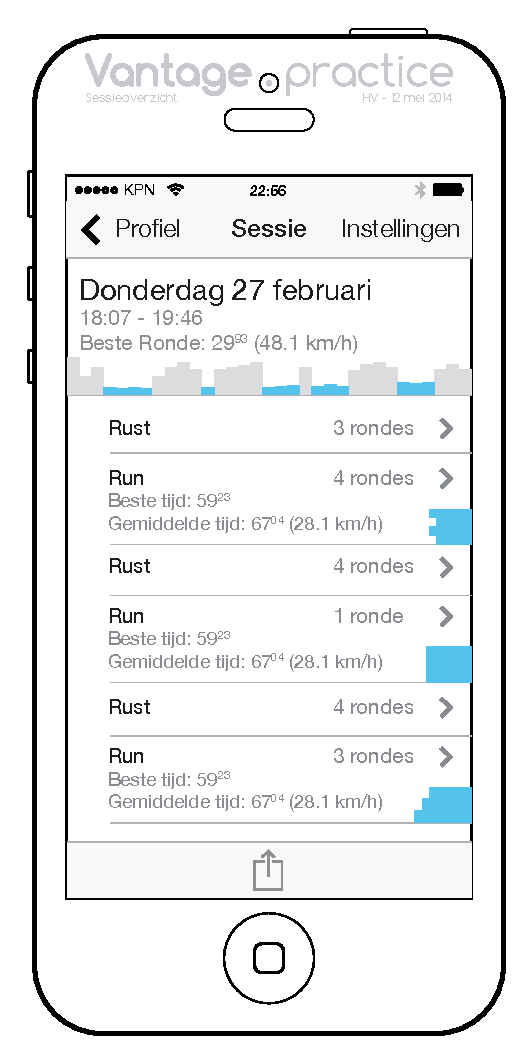
\includegraphics[width=4.5cm]{style/images/designs/06-Sessieoverzicht}
    \label{fig:ingeklapt-sessieoverzicht}
}
\subfigure[Sessieoverzicht met een opengeklapte run]{
    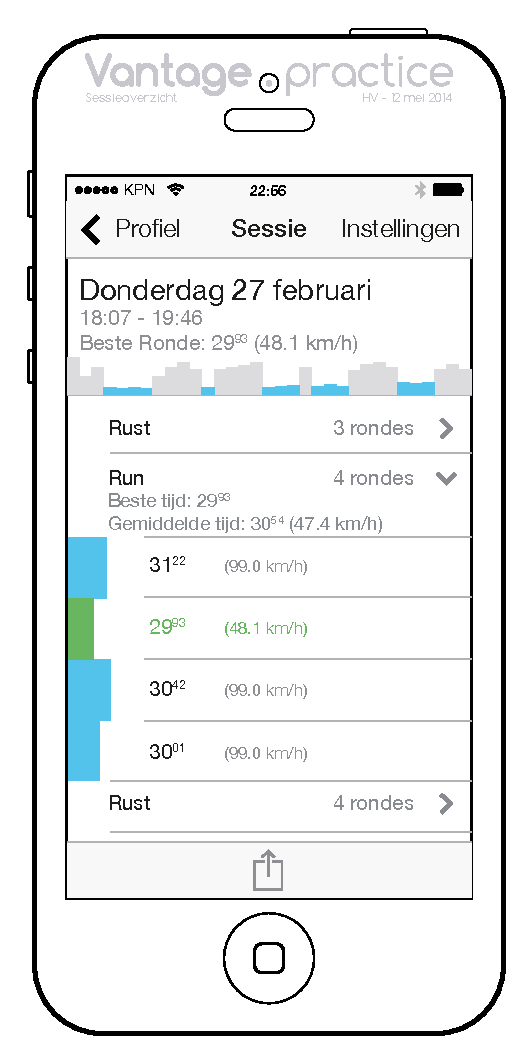
\includegraphics[width=4.5cm]{style/images/designs/07-Runoverzicht}
    \label{fig:uitgeklapt-sessieoverzicht}
}
\caption{Sessie-schermen}
\label{fig:sessie-schermen}
\end{figure}

\begin{figure}[ht]
\centering
\subfigure[Favorietenoverzicht]{
    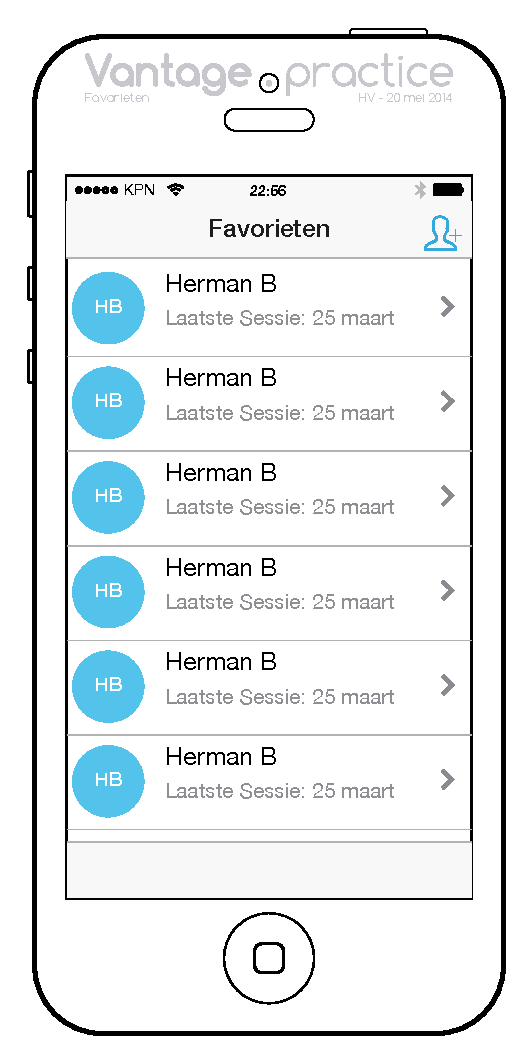
\includegraphics[width=4.5cm]{style/images/designs/09-Favorieten-A}
    \label{fig:favorieten-lijst}
}
\subfigure[Favorieten Toevoegen]{
    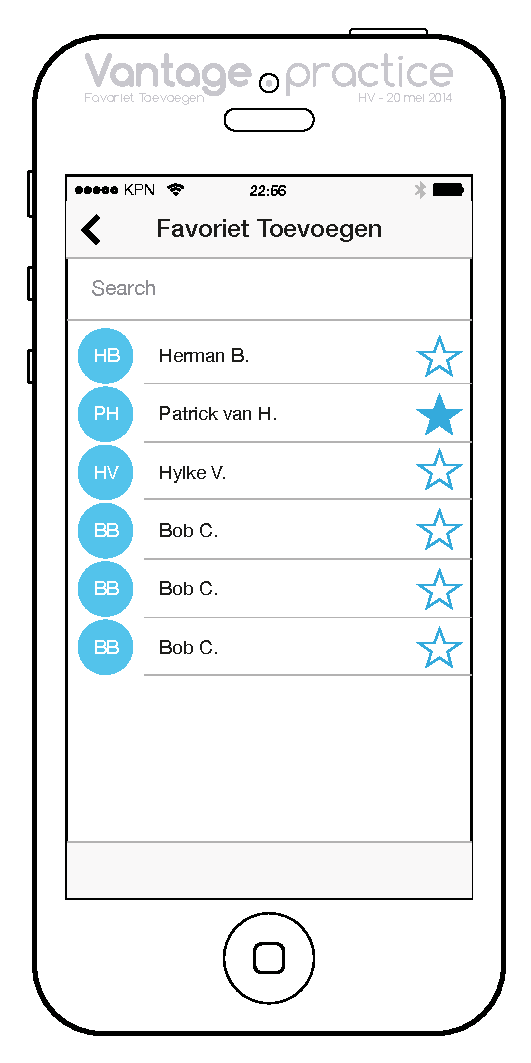
\includegraphics[width=4.5cm]{style/images/designs/09-Favorieten-B}
    \label{fig:favorieten-toevoegen}
}
\caption{Favorieten-schermen}
\label{fig:favorieten-schermen}
\end{figure}

\begin{figure}[ht]
\centering
\subfigure[Groepenoverzicht]{
    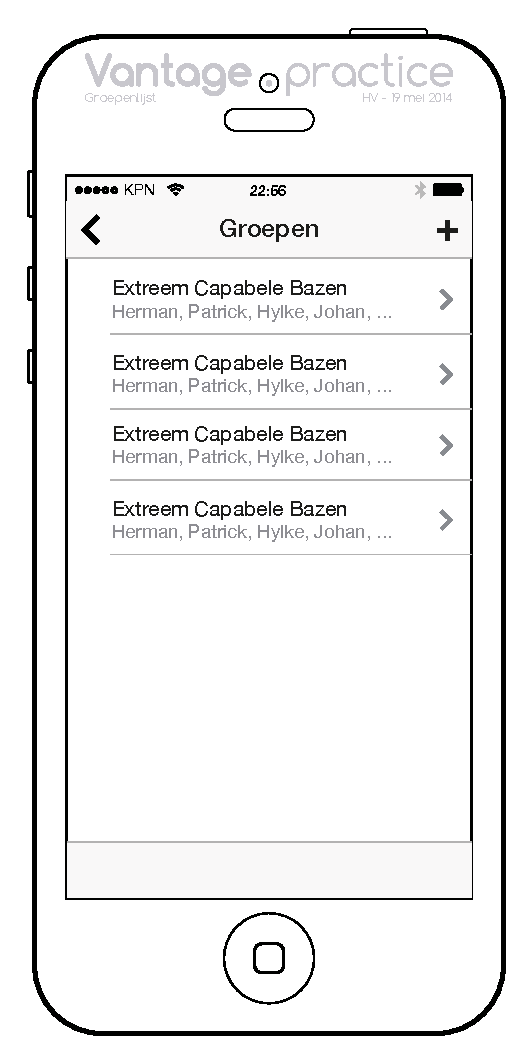
\includegraphics[width=4.5cm]{style/images/designs/12-Groepenlijst}
    \label{fig:groepenoverzicht}
}
\subfigure[Groep Detail]{
    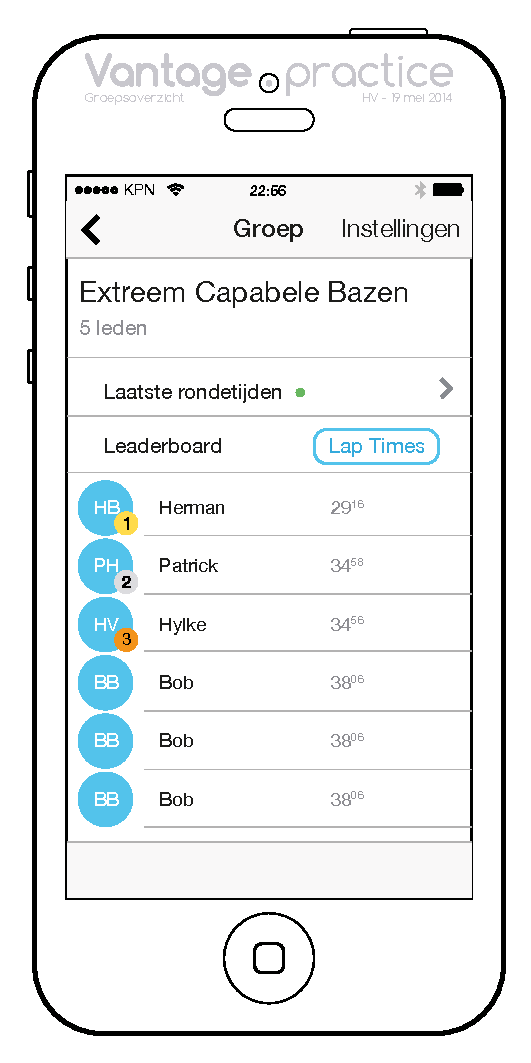
\includegraphics[width=4.5cm]{style/images/designs/13-Groep}
    \label{fig:groep-detail}
}
\subfigure[Groepsinstellingen]{
    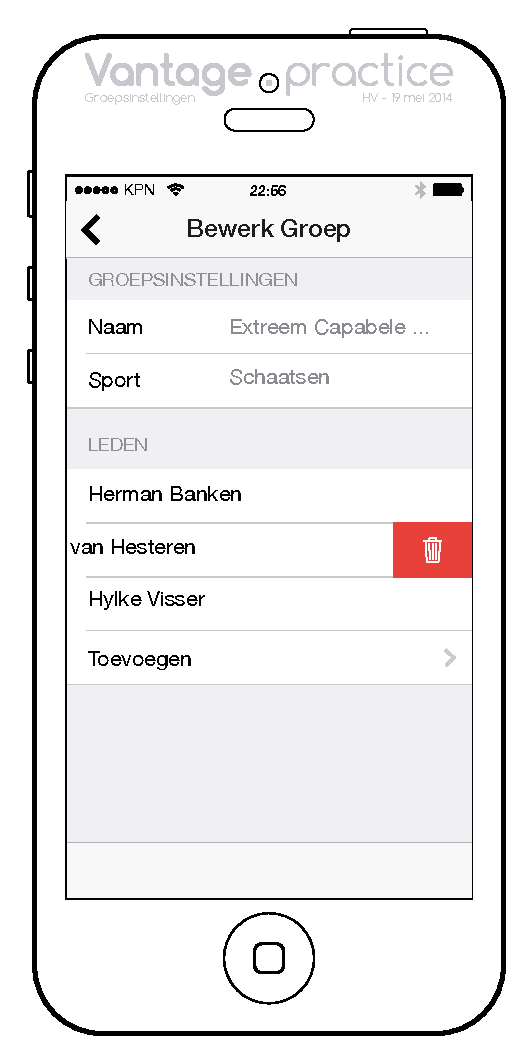
\includegraphics[width=4.5cm]{style/images/designs/14-Groepsinstellingen}
    \label{fig:groepsinstellingen}
}
\caption{Groeps-schermen}
\label{fig:groeps-schermen}
\end{figure}



\chapter{Testresultaten} \label{ch:testplan}
    \label{sec:enquete-resultaten}

Onderstaande tabel bevat de resultaten van de enquête. In totaal zijn er 31 enquête-formulieren ingeleverd. Sommige vragen waren multiple choice en sommige op basis van een schaal naar belangrijkheid, waar 1 onbelangrijk is en 5 erg belangrijk.

\begin{figure}[ht]
  \begin{center}
    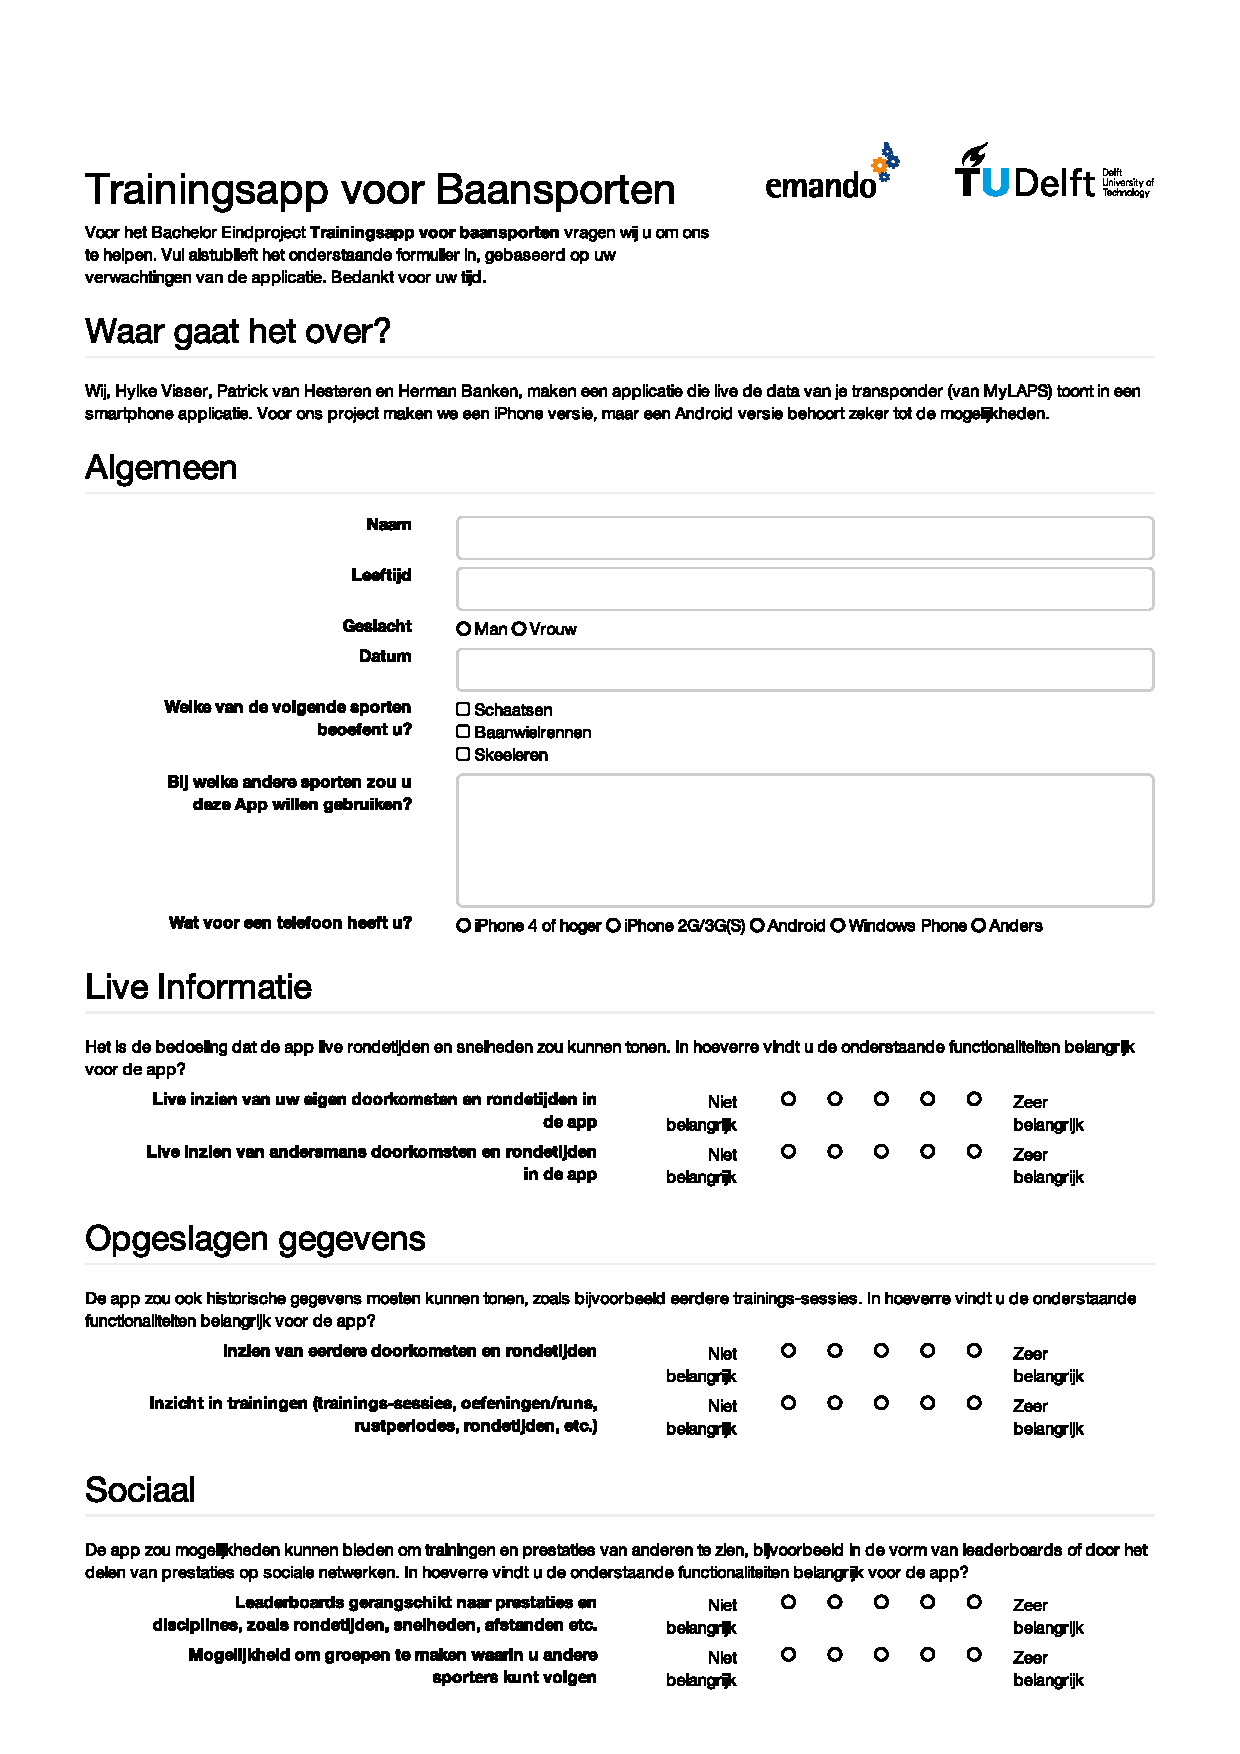
\includegraphics[width=\textwidth]{style/images/Enquete1}
  \end{center}
  \label{fig:enquete1}
\end{figure}

\begin{figure}[ht]
  \begin{center}
    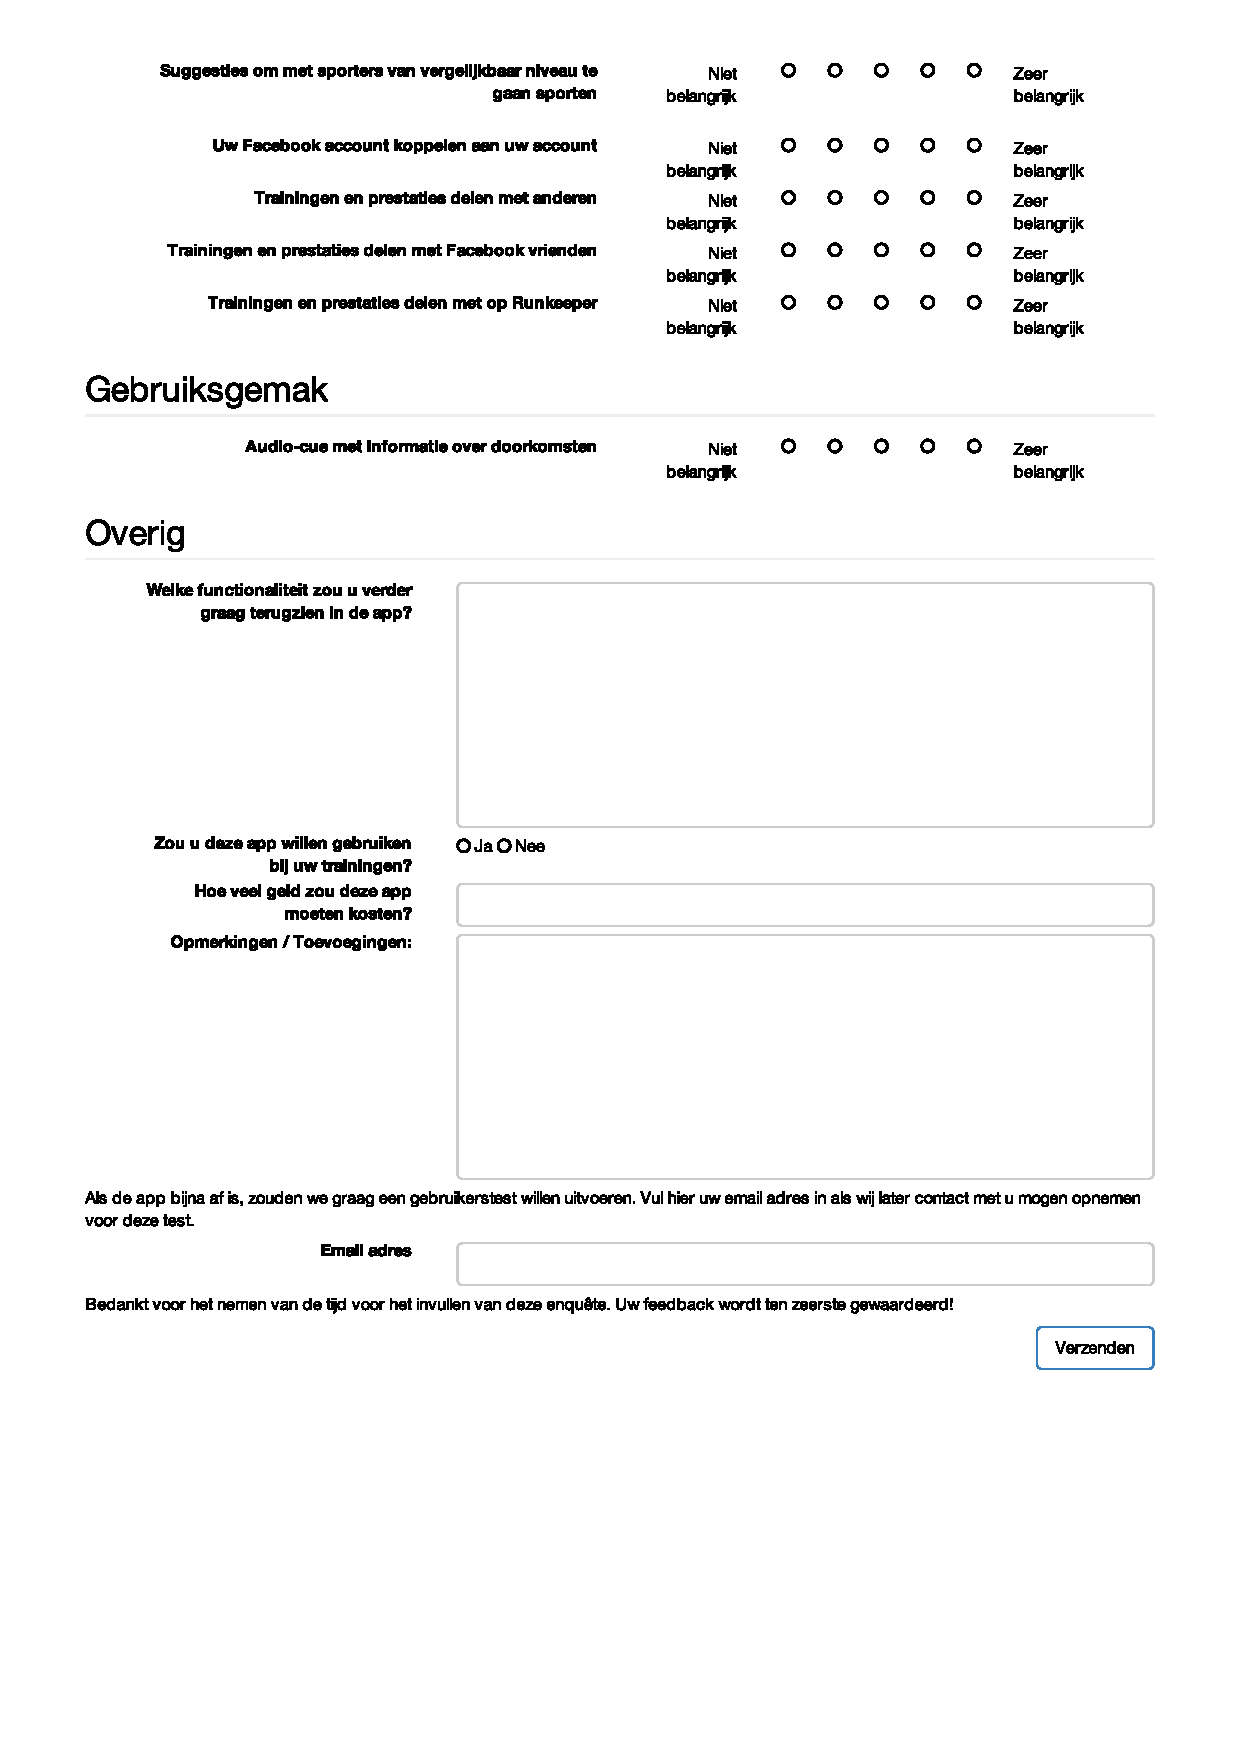
\includegraphics[width=\textwidth]{style/images/Enquete2}
  \end{center}
  \label{fig:enquete2}
\end{figure}

\begin{table}[h]
\begin{tabular}{| l | l | l |}
\hline
                         & \multicolumn{2}{l |}{Distributie of}                                                          \\ \hline
                         & Gemiddelde                                     & Standaard deviatie                           \\ \hline
\multicolumn{3}{l}{\textbf{Algemeen}}                                                                                  \\ \hline
Leeftijd                 & 24.1 jaar                                      & 9.0                                          \\ \hline
Geslacht                 & \multicolumn{2}{l|}{70\% man, 30\% vrouw}                                                     \\ \hline
Sporten                  & \multicolumn{2}{l|}{96.7\% Schaatsen, 66.7\% Skeeleren, 6,7\% Baanwielrennen}                 \\ \hline
Sporten overig           & \multicolumn{2}{l|}{Hardlopen, weg-wielrennen, athletiek}                                     \\ \hline
Telefoon                 & \multicolumn{2}{l|}{\begin{tabular}[c]{@{}l@{}}70.0\% Android, 23.3\% iPhone 4+\\ 3.3\% iPhone 2G/3G, 3.3\% Windows Phone\end{tabular}} \\ \hline
\multicolumn{3}{l}{\textbf{Live informatie}}                                                                           \\ \hline
Eigen doorkomsten        & 4.53 uit 5                                     & 0.73                                         \\ \hline
Andermans doorkomsten    & 3.47 uit 5                                     & 1.11                                         \\ \hline
\multicolumn{3}{l}{\textbf{Opgeslagen data}}                                                                           \\ \hline
Inzien doorkomsten       & 4.57 uit 5                                     & 0.63                                         \\ \hline
Inzicht in trainingen    & 4.30 uit 5                                     & 0.84                                         \\ \hline
\multicolumn{3}{l}{\textbf{Sociaal}}                                                                                   \\ \hline
Leaderboards             & 3.23 uit 5                                     & 0.94                                         \\ \hline
Groepen maken            & 3.83 uit 5                                     & 0.91                                         \\ \hline
Suggesties               & 2.73 uit 5                                     & 1.14                                         \\ \hline
Facebook login           & 2.13 uit 5                                     & 1.20                                         \\ \hline
Delen resultaten         & 2.67 uit 5                                     & 1.24                                         \\ \hline
Delen via FB             & 2.00 uit 5                                     & 1.20                                         \\ \hline
Delen via RunKeeper      & 1.63 uit 5                                     & 1.00                                         \\ \hline
\multicolumn{3}{l}{\textbf{Gebruiksgemak}}                                                                             \\ \hline
Audio-cue                & 3.83 uit 5                                     & 1.26                                         \\ \hline
\multicolumn{3}{l}{\textbf{Overig}}                                                                                    \\ \hline
De app willen gebruiken  & \multicolumn{2}{l|}{96.7\% ja, 3.3\% nee}                                                     \\ \hline
Wat de app mag kosten    & € 1.72                                         & 2.13                                         \\ \hline               
\end{tabular}
\end{table}

\newpage

\section*{Verdere functionaliteit opgegeven door respondenten}
\begin{itemize}
\item Tijdsverschillen tussen de rondjes (mobiel bij trainer en rondetijden gelijk terugkijken na oefening)
\item Actuele snelheid zou wel vet zijn. Of een verwachte rondetijd op basis van de huidige snelheid.
\item Trainingen en prestaties delen met endomondo
\item Hardslagmeter, calorieën-schatter. Suggesties voor trainingschema's: lange termijn (intensievere trainingsweek of extensievere trainingsweek) en korte termijn (schaats-schema's die te laden zijn en aan de prestatie gekoppeld worden).
\item Gebruiksvriendelijk, snelheid bv: snel opgestart, etc. De Hockey-WK-app is bijvoorbeeld erg traag en dat is echt niet fijn.
\item Vooraf ingesteld trainingsschema (wat nu gaan doen?) \item Tussentijdse feedback op rijden (tijdens het rijden een piep voor elke "100" meter (niet echt honderd meter, maar herkenbare punten: ingaan bocht/rechte eind, passeren van 1000m start, enz als je een bepaald tempo moet rijden bijvoorbeeld.
\item Tijdens training liever niet vergelijken met anderem, achteraf wel leuk.
\item Misschien een mogelijkheid om je trainingsschema vooraf in te vullen. Dan kun je vervolgens live zien of je dat ook aan het bewerkstelligen bent of dat je niet doet wat je moest doen. Chearleaders die je aanmoedigen als je een beetje achterop raakt op je schema en het boze hoofd van John de Wolf als je gefaald hebt zijn bonus.
\item Metingen op basis van gps en niet alleen via transponders (als dat mogelijk is, vooral handig voor skeeleren).
\item Misschien een rondeteller (zoals die oude mannetjes altijd hebben) voor als je veel rondjes gaat rijden en het zou ook wel vet zijn als je ook je hartslag erbij kan zien, maar dat is voor de echte pro's!
\end{itemize}

\section*{Overige opmerkingen door respondenten}

\begin{itemize}
\item Leuk bedacht, alleen jammer dat je er een transponder voor nodig hebt, wordt het gelijk wel duur. Zou dit ook met GPS kunnen?
\item Het zou wel geniaal zijn als je via je oortjes je hele trainingsschema te horen krijgt en deze vervolgens rijdt en dat de app weet hoe ver je steeds bent. En het lijkt me een vooruitgang dat je real-time weet hoe je snel je de afstanden aflegt, zodat je bijvoorbeeld een vlak of oplopend schema kan rijden.
\item Altijd met telefoon in de hand wordt de ijsbaan niet veiliger van. Denk goed na wanneer je je tel wel/niet in de hand hebt.
\item Een van de belangrijkste punten is wat mij betreft de audiofeedback tijdens het sporten. Het terugkijken van gereden tijden is leuk, maar direct feedback tijdens het sporten werkt voor mij (uit ervaring met RunTastic apps voor hardlopen en wielrennen) erg motiverend.
\item iPhone 4 en verder zijn in dit onderzoek onder een noemer gebracht. Ik merk nu al dat de RunTastic apps, die inmiddels geoptimaliseerd zijn voor iPhone 5C/S, behoorlijk trager werken op iPhone 4. Het zou geweldig zijn als deze app ook soepel runt op iPhone 4. 
\item Werkt de app ook zonder transponder, bijvoorbeeld op GPS?
\end{itemize}

\chapter{Aggregatie Flow} \label{ch:aggregation-flow}

\begin{figure}[ht]
  \begin{center}
    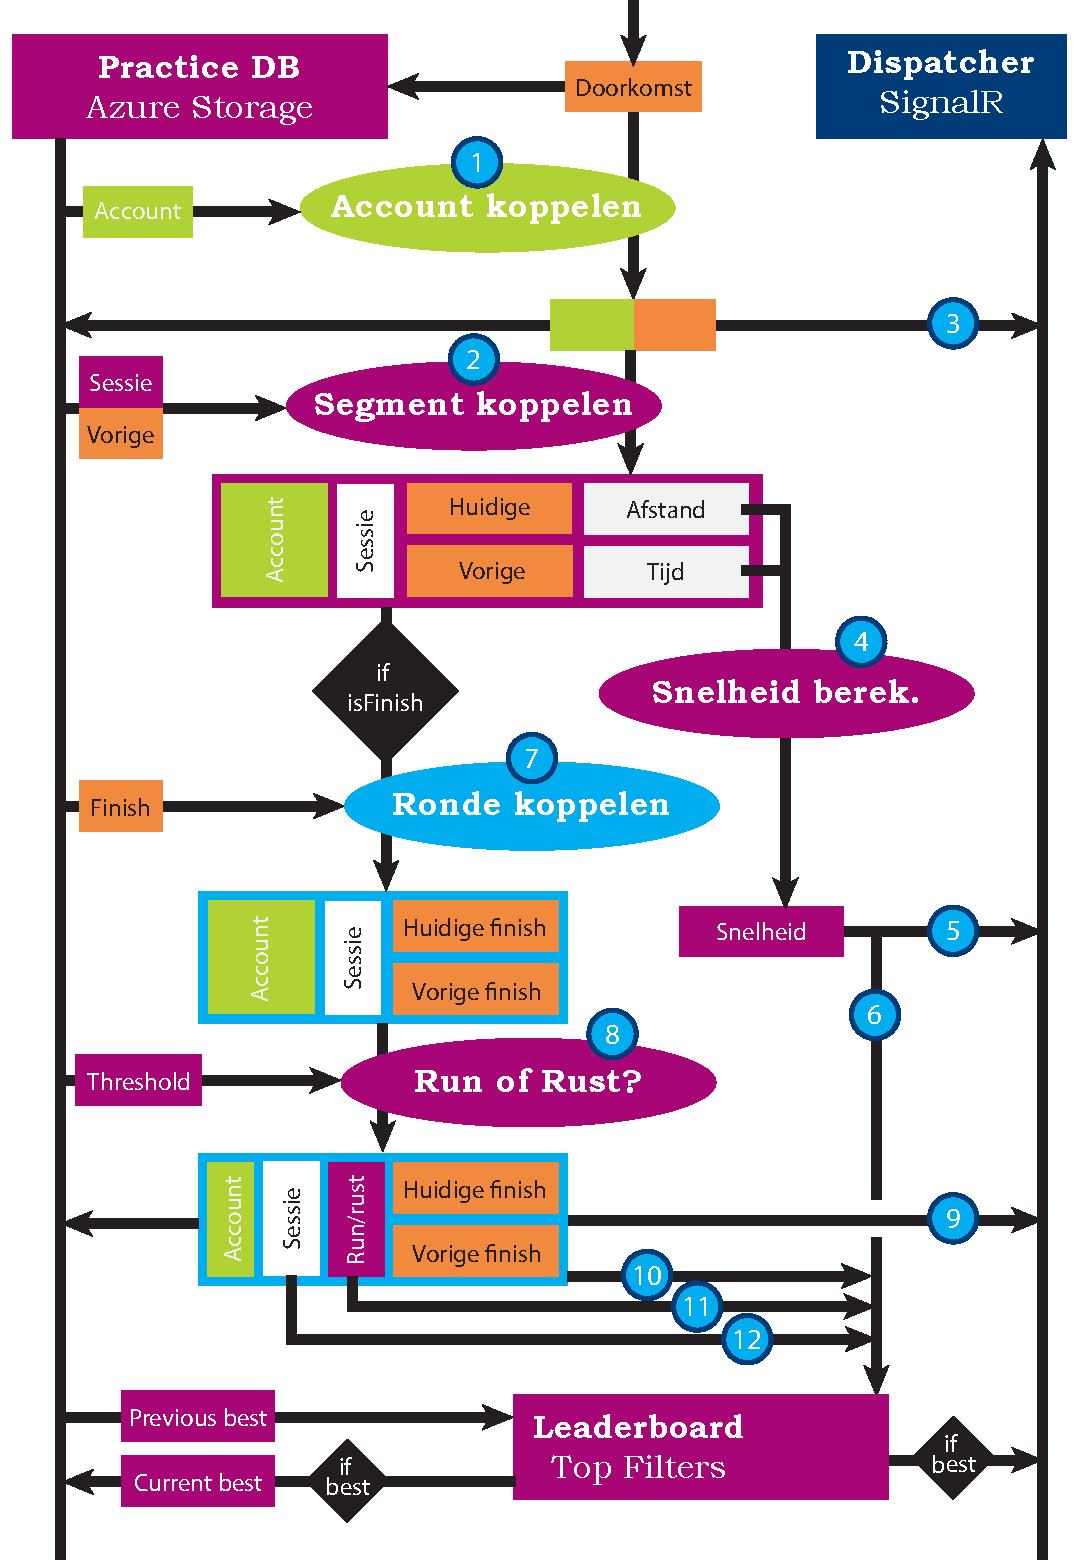
\includegraphics[width=\textwidth]{style/images/Aggregatie-flow}
  \end{center}
  \caption{Flow-diagram van het aggregatie proces}
  \label{fig:aggregatie-flow-large}
\end{figure}

\bibliography{references}

\end{document}